\chapter{Detector Installation}
\label{ch:sp-tc}

This chapter covers all the work and infrastructure required to install an SP detector module. 
Before getting into the details, we first provide some reminders of the scale of the task, beginning with the two facts that drive all others: A DUNE FD module is enormous, with outer cryostat dimensions length$\times $width$\times $height$=$ $62\times 19\times 18$ m$^{3}$; and every piece of the FD module must travel $1500$ \si{m} down the Ross shaft to the 4850 level of SURF and be transported to the detector caverns.

For the \dword{tpc}, 150 \dword{apa}s, each $6.0$ m high and $2.3$ m wide and  weighing $600$ kg with $3500$ strung sense and shielding wires, must be taken down the shaft as special \textquotedblleft slung loads\textquotedblright and moved to the area outside the \dword{dune} cryostat. 
The \dword{apa} are moved into a pre-prepared length$\times $width$\times $height$=$ $30\times 19 \times 17\ {\rm or}\ 10$ m$^{3}$ clean room where they are first be outfitted  with photon detector units and passed through a series of qualification tests.
Here two APAs are linked into a vertical 12 m high double unit, connect to readout electronics, receive a cold-test in place, and then move into the cryostat to be connected at the proper location on the previously installed detector support structure (DSS) and cabled up with the feedthroughs. 
In parallel the field cages that define the \dword{tpc} active volume must be installed with all their high voltage connections, along with  elements of the cryogenic instrumentation and slow control (CISC) and calibration systems.

After twelve months of detector component installation, which follows twelve months of detector infrastructure installation, the cryostat closes (with the last installation steps occurring in confined space accessed through a narrow human access port). 
Following leak checks, final electrical connection tests, and installation of the neutron calibration source, the process of filling the cryostat with $17,000,000$ kg of LAr begins.

From this terse summary, it is clear that installation requires meticulous planning and execution of thousands of tasks by well-trained teams of technicians, riggers, and detector specialists. 
High level requirements for these tasks are spelled out in Table \ref{tab:specs:just:SP-TC} and the text that follows. 
In all the planning and future work the requirement that subsumes all others in the installation process is safety safety. DUNE's goal is zero accidents resulting in personal injury, damage to detector components, or harm to the environment.

% This file is generated, any edits may be lost.

\begin{longtable}{p{0.14\textwidth}p{0.13\textwidth}p{0.18\textwidth}p{0.22\textwidth}p{0.20\textwidth}}
\caption{Specifications for SP-TC \fixmehl{ref \texttt{tab:spec:SP-TC}}} \\
  \rowcolor{dunesky}
       Label & Description  & Specification \newline (Goal) & Rationale & Validation \\  \colhline

   
  \newtag{SP-TC-1}{ spec:logistics-material-handling }  & Compliance with the SURF Material Handling Specification for all material transported underground  &  SURF Material Handling Specification &  Loads must fit in the shaft be lifted safely. &  Visual and documentation check \\ \colhline
     % 1
   
  \newtag{SP-TC-2}{ spec:logistics-shipping-coord }  & Coordination of shipments with CMGC; DUNE to schedule use of Ross Shaft  &  2 wk notice to CMGC &  Both DUNE and CMGC need to use Ross Shaft &  Deliveries will be rejected. \\ \colhline
     % 2
   
  \newtag{SP-TC-3}{ spec:logistics-materials-buffer }  & Maintain materials buffer at logistics facility in SD   &  $>1$ month &  Prevent schedule delays in case of shipping or customs delays &  Documentatation and progress reporting \\ \colhline
     % 3
   
  \newtag{SP-TC-4}{ spec:apa-storage-sd }  & APA stroage at logistics facility in SD  &  na &  Store APAs during lag between production and installation &  Agree upon space needs. \\ \colhline
     % 4
   
  \newtag{SP-TC-5}{ spec:cleanroom-specification }  & Standard for ITF and installation cleanrooms  &  na &  Reduce dust (contains U/Th) to prevent induced radiological background in detector &  Monitor air purity \\ \colhline
     % 5
   
  \newtag{SP-TC-6}{ spec:cleanroom-uv-filters }  & UV filter in ITF and installation cleanrooms for PDS sensor protection  &  na &  Prevent damage to PD coatings  &  Visual or spectrographic inspection \\ \colhline
     % 6


\label{tab:specs:just:SP-TC}
\end{longtable}
\fixme{Anne needs to fix the figure caption for specifications} 
\fixme{Jim needs to fix the specification for TC 5and 6} 
Installation of the DUNE FD presents a multitude of hazards that includes  manipulation heavy loads in the tight spaces of the mine and detector module,  working at considerable heights above the floor, repeated utilization of large volumes of cryogens, multiple tests with high voltage, commissioning of a class IV laser system, and deployment of a high activity neutron source. Mitigation of these hazards begins with the strong professional on-site ES\&H\ teams of the Fermilab South Dakota Services Division (SDSD) and the host SURF lab.
All installation team members, both at the surface and underground, will undergo rigorous formal safety training that will be update at daily intervals. Any team member can stop work at any time for safety purposes. Further details of the overall DUNE safety plan are provided in Chapter 9 of the Technical Coordination Volume of the TDR. In addition, each section of this chapter provides further details on the evolving safety plan for installation. This plan has been informed by the successful safety experience of SURF with other underground experiments (e.g., LUX, Majorana Demonstrator, LZ), DUNE members in executing projects at other underground locations (e.g., MINOS at Soudan, Minnesota, USA), at other locations remote from major international laboratories (e.g., Daya Bay, China and No$\nu $a Far Detector (Ash River, Minnesota, USA), and at the home laboratories of both Fermilab and CERN.


% risk table values for subsystem SP-FD-JPO
\begin{longtable}{p{0.15\textwidth}p{0.13\textwidth}p{0.13\textwidth}p{0.28\textwidth}p{0.06\textwidth}p{0.06\textwidth}p{0.06\textwidth}} 
\caption{Specification for SP-FD-JPO \fixmehl{ref \texttt{tab:specs:SP-FD-JPO}}} \\
\rowcolor{dunesky}
ID & Risk & Label & Mitigation & Prob ability & Cost Impact & Sched ule Impact \\  \colhline
RT-JPO-001 & Personnel injury & jpo-person-injury & Follow established safety plans. & M & L & H \\  \colhline
RT-JPO-002 & Shipping delays & jpo-shipping-delay & Plan one month buffer to store  materials locally. Provide logistics manual. & H & L & L \\  \colhline
RT-JPO-003 & Missing components cause delays & jpo-missing-components & Use detailed inventory system to verify availability of  necessary components.  & H & L & L \\  \colhline
RT-JPO-004 & Import, export, visa issues  & jpo-import-visa & Dedicated \dword{fnal} \dword{sdsd}division will expedite import/export and visa-related issues. & H & M & M \\  \colhline
RT-JPO-005 & Lack of available labor  & jpo-labor-avail & Hire early and use Ash River setup to train \dword{jpo} crew. & L & L & L \\  \colhline
RT-JPO-006 & Parts do not fit together & jpo-cannot-assemble & Generate \threed model, create interface drawings, and prototype detector assembly. & H & L & L \\  \colhline
RT-JPO-007 & Cryostat damage & jpo-cryostat-damage & Use cryostat false floor and temporary protection. & L & L & M \\  \colhline
RT-JPO-008 & Weather closes SURF & jpo-weather-delay & Plan for \dword{surf} weather closures & H & L & L \\  \colhline
RT-JPO-009 & Detector failure during \cooldown & jpo-cooldown-failure & Cold test individual components then cold test \dword{apa} assemblies immediately before installation. & L & H & H \\  \colhline

\label{tab:risks:SP-FD-JPO}
\end{longtable}
\fixme{Anne needs to fix the figure caption for risks} 

As part of the \dword{dune} design process the detector components and the TPC have been prototyped at various stages. The \dword{protodune}-SP prototype which was assembled from full scale dune components has recently been completed and has taken data. 
This process has been extremely important in planning the far detector installation. A detailed list of lessons learned from \dword{protodune}-SP construction and installation was compiled.\cite{bib:docdb8255} 
These lessons learned and other experience from the team planning the installation was used to develop a list of \textquotedblleft risks \textquotedblright for the \dword{dune} installation. 
The risk register documents what could be improved from the \dword{protodune} installation and what people felt could go wrong in the \dword{dune} installation. After the list of risks are generated plans to prevent the risks from occurring or minimizing the impacting to the project are formulated as mitigation strategies. These plans to improve what was done in \dword{protodune} or prevent difficulties at \dword{dune} are then built into the \dword{dune} installation plan. The list of risks associated with the \dword{dune} installation are shown in Table \ref{tab:INSTALL-risks}. The risks in Table \ref{tab:INSTALL-risks} are considered the highest impact risks where a dedicated mitigation strategy is required. All the lessons learned from \dword{protodune} will be factored into the detailed installation planning.
\fixme{Anne needs to add the correct label for the ref}

This  installation chapter is divided into three main sections describing the main divisions of work. First the logistics section describes how material will be delivered to the South Dakota region and then forwarded to the Ross headframe on the \dword{surf} site for transport underground. A warehouse facility is used for buffering materials prior to transport to \dword{surf}, inventorying shipments, consolidating packages, and coordinating with the  \dword{cf}-\dword{cmgc}. The second section describes all the infrastructure needed to install and operated the detector. This includes the cleanroom for installation and its contents but also infrastructure like racks, cable trays, storage facilities and machining facilities. The third section describes the actual installation process itself which is divided into 3 phases: the \dword{cuc} setup phase, the installation setup phase, and the detector installation phase. 


\section{Logistics}
\label{sec:fdsp-tc-log}

%%%%%%%%%%%%%%%%%%%%%%%%%%%%
\subsection{Introduction}
\label{sec:fdsp-tc-log-intro}
The transportation of equipment and people underground is one of the more challenging aspects of the LBNF/DUNE endeavor. The access underground is via the mile long Ross shaft, which is now undergoing renovation. The shaft is outfitted with a single cage for people and materials and two skips which are needed for removing the rock underground. Planning the usage of the cage is one of the most important exercises in making LBNF/DUNE a success. Given the enormous cost of the conventional facilities (CF) contracts and the large cost of any in-efficiencies in construction the overall coordinator of the Ross Shaft for LBNF/DUNE will be the CF Central Manager General Contractor (CMGC). Independent of CF both LBNF and DUNE have a large number of contractors, institutions, and scientists who will need to bring equipment and materials underground. In order to facilitate the flow of material and people to the underground area a logistics organization will be established in South Dakota near SURF. This organization will be responsible for receiving all goods for LBNF (except CF) and DUNE, it will be responsible for coordinating the transport of this material underground with the CF-CMGC, and it will coordinate personnel usage of the Ross cage with the CF-CMGC. 


\begin{dunetable}
[Logistics Specifications]
{cc}
{tab:table-Log-Req}
{Table of logistics specifications.}
Specifications &  \\ \toprowrule
Material Handling & Comply with the SURF Material Handling Specification \\ \colhline
CMGS coordination & Provide CMGC with 2 week notice of shipments to SURF \\ \colhline
Stage DUNE Shipments & Provide a 1 month local buffer of DUNE materials \\
\colhline
APA Storage & Provide storage space for 150 APA in a clean environment \\
\colhline
Inventory & Provide an inventory system accessible to the collaboration \\
\end{dunetable}
 \fixme{Specifications table needs to be converted to official format}
 
 A high level overview of the material flow to the Ross shaft is shown in Figure \ref{fig:logistics-material-flow}. Freight is delivered to a central South Dakota Warehouse Facility (SDWF) with possible exception of the cryogenic equipment. The materials are then transported in a "just--in--time" fashion to the Ross headframe where they are brought underground. For the detector the APA electronics and photon detector components will also be shipped to the Integration Test Facility where they are assembled and then shipped back to SDWF.
 
\begin{dunefigure}[Material Flow Diagram ]{fig:logistics-material-flow}
  {Material Flow diagram for the LBNF/DUNE logistics.}
 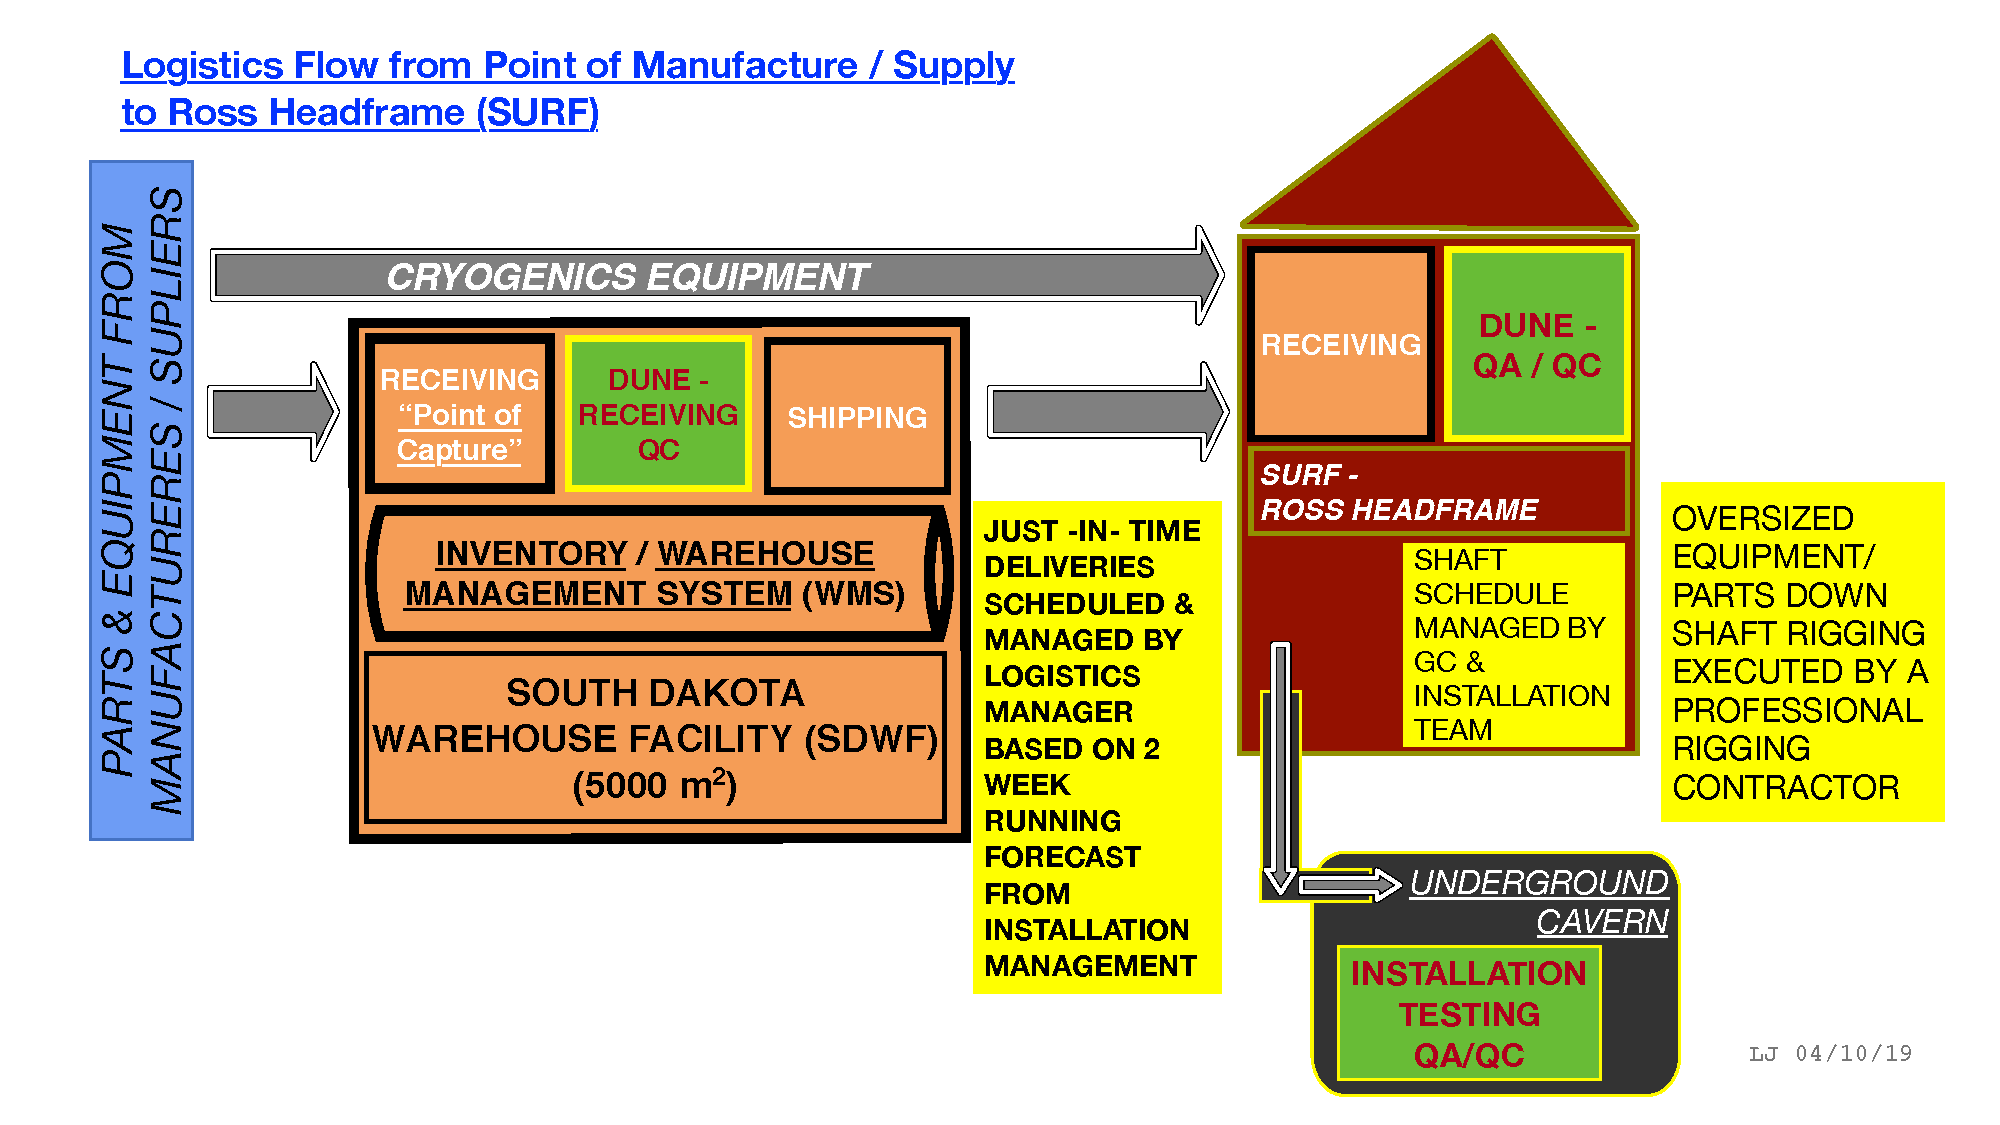
\includegraphics[width=\textwidth]{logistics-material-flow}
\end{dunefigure}


%%%%%%%%%%%%%%%%%%%%%%%%%%%%
\subsection{Logistics Planning}
\label{sec:fdsp-tc-logPln}
The LBNF/DUNE Logistics scope includes overseeing the transportation of the cryostat (steel, foam, and membrane), the cryogenic system, the detector, and all related infrastructure not provided by facilities. The LBNF scope consists of the cryostat and cryogenics and it will not be discussed in detail in this TDR but as the LBNF material dominates the logistics needs a brief summary here is required. The cryostat steel structure for each cryostat requires bringing roughly 1,800 individual steel pieces underground some which weigh up to 7.5t and 125t of bolts needed to assemble the steel pieces. The internal structure which includes the foam insulation and the thin stainless steel membrane will require transporting roughly 4,000 boxes each roughly 1.5 $\times$ 3.5 $\times$ 1.2 m$^3$ in dimension. The plan for cryostat installation at present calls for all the components to be warehoused in SD prior to the start of installation. This means that the logistics operation will need roughly 5,000 m$^2$ of warehouse space roughly 2 years prior to the start of DUNE detector installation. By the time DUNE detector components start arriving most the cryostat boxes will have been removed from the warehouse so there will be ample space for the detector and cryogenics components. Additional space may be required if the boxes for the second cryostat arrive before the detector\#1 installation is complete, but several buildings of the required size are available in the area if it is decided expansion is required.


\begin{dunefigure}[Ross Cage]{fig:fdsp-tc-Cage}
  {Simplified model of the new Ross Cage.}
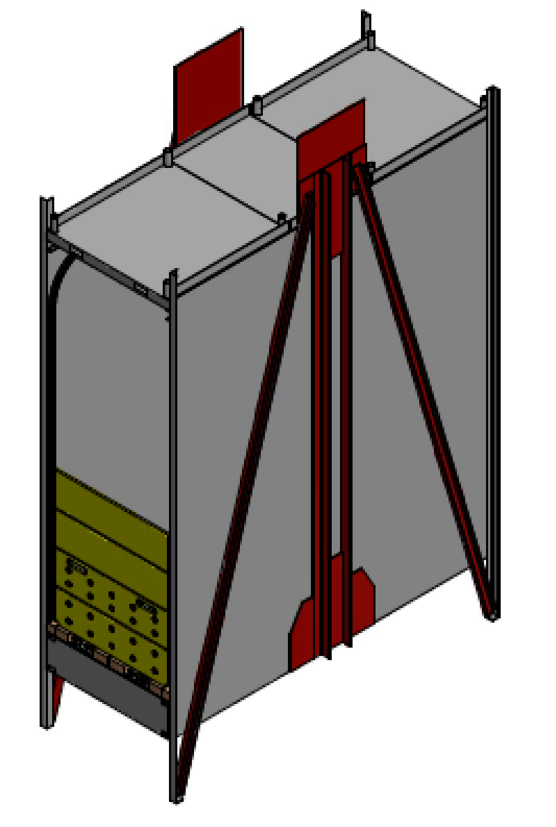
\includegraphics[width=.5\textwidth]{Cage-view}
\fixme{combine with table?}
\end{dunefigure}
%
\begin{dunetable}
[Ross Cage Specifications]
{cc}
{tab:table-Ross-Cage}
{Table of parameters for the Ross hoist and cage.}
Ross Cage Parameters &  
\\ \toprowrule
Inside height &  3.6 m\\ \colhline
Inside depth & 3.7 m \\ \colhline
Inside width & 1.38 m \\
\colhline
Weight limit&  5,897 kg \\
\colhline
Round trip time & 17 min\\ \colhline
\end{dunetable}

All material brought underground must conform to the Sanford Underground Research Facility's (SURF) Facility Access Specification \cite{bib:docdb328}. This document defines the limitations on dimensions and weights for all materials to be transported underground.  The most important limitations which are described in detail in the specification document are related to the Ross shaft and Ross cage. It is possible to bring material down the shaft outside the cage as a slung load but this is a much slower process and requires careful planning, detailed procedures and review. The DUNE APA for example need this special handling as they are too tall to fit in the cage. Most material should be brought underground in the cage. Figure \ref{fig:fdsp-tc-Cage} shows an image of the new Ross cage and Table \ref{tab:table-Ross-Cage} summarizes its parameters. As a comparison the round trip travel time for the Ross cage is 17 minutes where most the time needed to load and unload the cage and any slung load will take over an hour round trip as both the loading/unloading and travel times are longer. 

Many other factors need to be considered when planning the DUNE logistics. There is no loading dock at the Ross headframe so all materials will need transported using a flatbed or curtain-sided truck. The equipment can then be removed using a forklift at SURF. In general one should plan on loading the trucks at the logistics warehouse in the same manner as they will be unloaded at SURF to ensure that there will be no unexpected difficulties. The CF-CMGC has to coordinate all the loads through the Ross shaft and to do this they will need to know 2 weeks in advance what is planned for DUNE in order to make the overall hoist schedule. It will also be forbidden for DUNE collaborators to ship equipment directly to the Ross Shaft unless this is coordinated by the DUNE logistics team. A central inventory system will capture all goods at receipt to the warehouse in South Dakota. DUNE institutions need to provide shipping data and consign cargo accordingly (a shipping manual will be provided by the logistics team) so that the logistics team can monitor the progress. In ProtoDUNE-SP delays in shipping and customs caused up to 3 weeks delay in arrival of some parts which caused significant re-planning of the installation work. In order to prevent this from being a much larger problem in DUNE a minimal one month buffer of materials will be planned. With this the underground work can be planned well in advance knowing all the materials will be available. This will require that sufficient space be available in the warehouse and underground at SURF to house the material buffer. Many small parcels will arrive at the warehouse. The warehouse staff will consolidate deliveries to SURF into larger boxes/crates, as per the SURF delivery plan, to make efficient use of the hoist. 


\begin{dunefigure}[Material for Setup]{fig:fdsp-tc-setup}
  {Image showing the cavern on end opposite of the detector. During the installation setup phase half the space will be used for the cryostat work and half as storage for the detector infrastructure. The material outside the cavern must be stored in the logistics warehouse.}
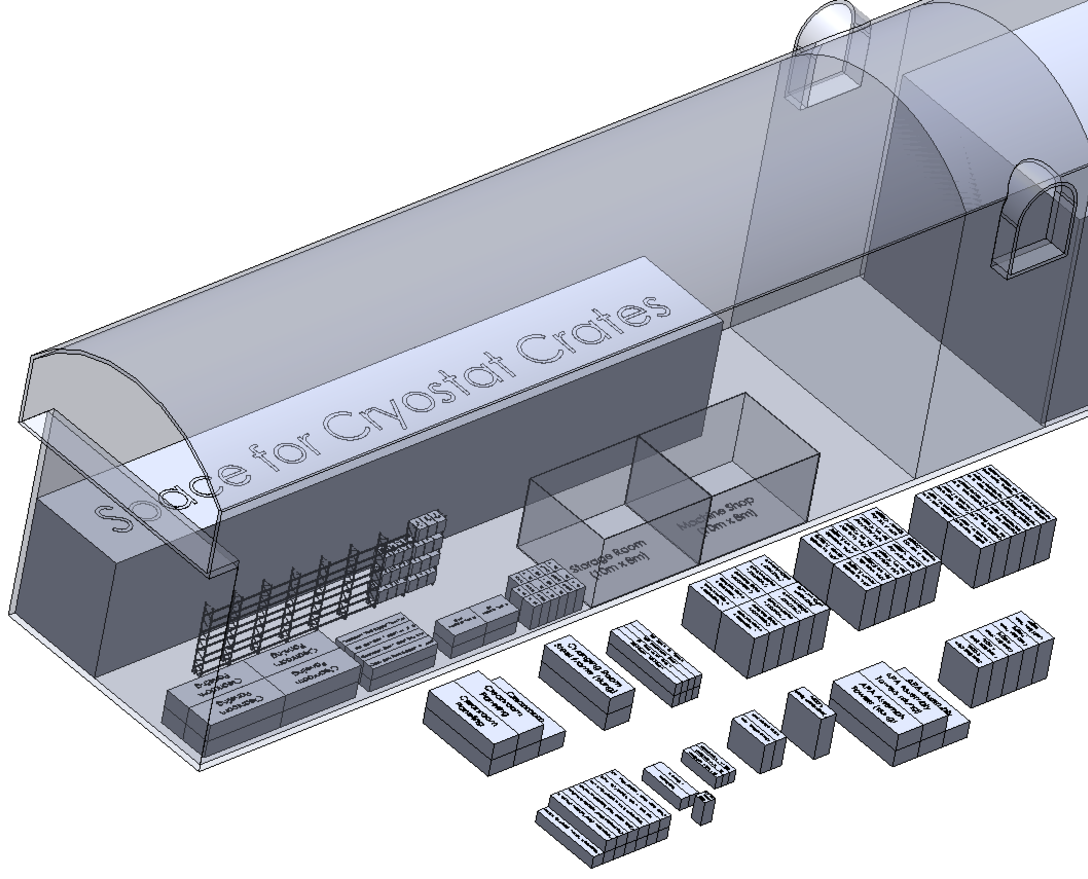
\includegraphics[width=.9\textwidth]{Material-Setup}
\end{dunefigure}
%

In order to understand how much space is needed for storage and how much of the hoist time must be dedicated to DUNE a detailed inventory of all the detector equipment and DUNE infrastructure is needed. The list of all the materials was solicited from all the consortia and technical coordination. The entries in the inventory spreadsheet are organized as "Loads" for the Ross shaft where a load is a crate or set of boxes which will either be transported underground in the hoist or as a slung load.\cite{bib:docdb8426}
%\href{http://docs.dunescience.org/cgi-bin/ShowDocument?docid=8426}{DUNE load Spreadsheet} \cite{bib:docdb8426}

Information captured in the Load spreadsheet includes the number of hoist trips, nature of the trip (slung load or cage), the package dimensions, weight and type of package (crate, pallet, pallet box). The load list at present accounts for 1,600 hoist trips and accounts for roughly 2 months of cage time most of which is spread over one year. The installation operation for the single-phase detector will span over 2 years so it is prudent to divide the logistics planning in several phases. The load information is divided into the CUC setup phase, the installation setup phase, and the detector installation phase. In each phase a model was generated to show how much material can be stored underground outside the work area and also how much material needs stored on the surface. These models are used to set the space requirements for the logistics effort on the surface. The phase with the largest amount of material to transport is the detector setup phase and the model of the underground area and the required boxes for surface storage for the first $1/3$\ of the setup is shown in Figure \ref{fig:fdsp-tc-setup}. This represents the first month of installation setup and shows that roughly 1,000 m$^2$\ of warehouse space will be needed for DUNE at this time. In addition to the space needed for receive and ship equipment underground the warehouse will also need space to store up to 150 APA. This adds an additional 700 m$^2$\ to the needed warehouse area. 


%%%%%%%%%%%%%%%%%%%%%%%%%%%%
\subsection{Quality Assurance and Quality Control}
\label{sec:fdsp-tc-itf-qaqc}


ProtoDUNE was an extremely useful exercise in general, but only a few conclusions can be drawn related to logistics since shipping to Europe will be different than shipping to South Dakota and the CERN receiving and transport divisions will not be used for DUNE. The most important lessons learned from ProtoDUNE related to logistics are listed below.
\begin{enumerate}
\item Lack of a central inventory system made it impossible to track shipments.
\item Delays in shipping meant that the installation work could not be planned and parts were installed as they arrived. 
\end{enumerate}

To address these issues an inventory system will be implemented at the logistics warehouse facility and a minimum one month material buffer will be required from the consortia in South Dakota.

It is not foreseen to do component testing in the warehouse so the scope of the quality control work there is limited. But there will have to be QA/QC component at receiving. One critical QC check that will be performed at the logistics facility is a check to ensure that all materials to be shipped to the Ross headframe will fit in the cage. Additionally if a slung load is needed the facility will confirm that the necessary procedures are in place and approved before any material is transported to SURF. The other primary QC function performed at the logistic facility is the inventory of all shipments described below.

The nature of this project with the "contribution in kind" model makes the logistics and inventory control as well as gathering of the relevant "construction" data extremely complex. Therefore, the logistics (inventory) control and scientific data collection need to be controlled by independent systems. 
The logistics supply chain will be controlled by the contributors freight forwarding system till arrival at the (yet to be defined/established) "South Dakota Warehouse Facility" (SDWF).  SDWF will be the ultimate "Point of Capture" for all LBNF/DUNE parts/equipment with the possible exemption the Cryogenic system as per the contractual requirements.
The inventory process at the SDWF, the ITF and the SURF receiving at Ross Shaft will be controlled by one integrated commercial Warehouse Management System (WMS), There will be need for some workflow functionality at ITF pre-assembly.
The Warehouse Management System (WMS/inventory) will provide basic receiving, inventory and shipping status information for all parts/equipment delivered to SDWF. That will include pre-assembled equipment that will enter as "new" parts from ITF as created by the work flow.
The QC/QA, manufacturing and other relevant data required/needed/desired by the DUNE collaboration will be stored in a separate yet to be defined and developed DUNE construction database. 
This DUNE construction database is independent of the WMS system and the relevant contributing consortia have the responsibility to transfer the required data prior to shipment from supplier to the DUNE construction database (DCDB).  The WMS database will provide the relevant/required/desired logistics data to the DCDB. The form of data transfer is yet to be determined.
All QC/QA, test and other relevant manufacturing data will be direct input into DCDB and will be the responsibility of the different contributing consortia (DUNE). DUNE will have to provide a QC/QA process for all parts/equipment received at the warehouse after being inventoried. That QC/QA data must be transfer directly to DCDB by DUNE. 
The DCDB will be an integral part of the logistic, assembly and QC/QA system. It will need to provide the ITF shipping (supply) and assembly reports as well as create the new "equipment" denomination for the WMS to register.  The DCDB will document the ITF subassembly process in its entirety (workflow).
The "new" sub-assembled items will be inventoried in WMS as new items during the warehouse receiving process.
The SURF installation management team will be responsible for providing a shipping (supply) report to the warehouse for scheduling of parts/equipment shipments to SURF.
The shipments from SDWF to SURF will be inventoried as received at SURF in WMS.
The DUNE installation team has to transfer the relevant QC/QA, test and installed status data to the DCDB directly.
To capture all relevant construction and logistics data on parts/equipment the following process for the logistics information is foreseen:

\begin{itemize}
\item The consortia must enter data related to any shipment to the SDWF in the WMS.
\item The shipments from SDWF to SURF will be inventoried as received at SURF in the WMS.
\item The SURF installation management team will be responsible for providing a shipping (supply) report to the warehouse for scheduling of parts/equipment shipments to SURF 2 weeks in advance of any shipment.
\end{itemize}







%%%%%%%%%%%%%%%%%%%%%%%%%%%%
\subsection{Safety}
\label{sec:fdsp-tc-itf-safety}

The LBNF/DUNE Logistics Facility is operated as a Fermilab Facility, but because of the international presence, we also follow CERN HSE, Fermilab ES\&H and SURF ES\&H regulations.  Work is in progress to combine all of this into a coherent list of codes and requirements to follow. The \dword{dune} Project ES\&H Coordinator has overall ES\&H oversight responsibility for the DUNE Project.  This person coordinates any activities and facilitates the resolution of any issues that cut across various Divisions and institutions. It is subject to the requirements of the DOE Workers Safety and Health Program, Title 10, Code Federal Regulations (CRF) Part 851 (10 CFR 851). These requirements are promulgated through the Fermilab Directors Policy Manual and Fermilab ES\&H manual (FESHM) which align with the SURF ES\&H Manual. 
Using the NOvA Far Detector Lab as a guideline for remote facilities there are several other key documents that guide the Logistics Center Safety Program.  The Building Safety Plan combines all of the building specific documents in a single folder:

\begin{enumerate}
\item	Fire Safety and Building Emergency Evacuation Plan- Fire evacuation plan, fire safety plan and lockdown plans, site plan
\item	Hazard Analysis- Describes all the typical hazards and their mediation including procedures 
\item	SDS- Safety Data Sheets
\item	Respiratory Plan- As required due to chemical or ODH hazards
\item	Training Program- Covers certifications required and  training records
\end{enumerate}

The current Technical Coordination facilities management plan has a joint safety officer used between the ITF and Logistics facility. This safety officer would facilitate training, write Hazard Analysis documents, run the weekly safety meetings, and keep documentation records on materials handling equipment and personnel. 


%%%%%%%%%%%%%%%%%%%%%%%%%%%%
\subsection{Cost, Schedule and Risk Analysis}
\label{sec:fdsp-tc-itf-cost}

\fixme{use templates from cost-risk-sched.tex file. Anne}


\section{Infrastructure}
\label{sec:fdsp-tc-infr}


%%%%%%%%%%%%%%%%%%%%%%%%%%%%
\subsection{Introduction}
\label{sec:fdsp-tc-infr-intro}

\fixme{Shop, Storage, 4850 infrastructure, diagnostic eq}
%%%%%%%%%%%%%%%%%%%%%%%%%%%%
%\subsection{Detector Support System}
\subsection{Detector Support System}
\label{sec:fdsp-tc-infr-dss}


The \dword{dss} provides the structural support for the detector inside the cryostat.  
It also provides the necessary infrastructure inside the cryostat to move the detector elements into place during assembly. 
The \dword{dss} is a new design, quite different from the \dword{pdsp} \dword{dss}. The detector elements supported by the \dword{dss} include the \dwords{ewfc}, the \dword{apa}s, and the \dword{cpa}s with top and bottom \dword{fc} panels. 
The nominal load of the detector elements both dry (in air) and wet (in \dword{lar}) are shown in Table \ref{tab:installation-DSS-load}. 
The weights listed are the current design weights.  
The \dword{dss}, however, is designed to accommodate significant design changes, even if the detector weight  doubles the \dword{dss} would still meet the design code requirements.  
Deformations would increase due to any increase in loads, and this effect would be evaluated if needed.

\begin{dunetable}
[DSS Loads]
{l|c|cc|cc}
{tab:installation-DSS-load}
{The expected dry and wet stratic loads for the DSS.}
%\multicolumn{2}{c}{} &  \multicolumn{4}{|c}{Dry Weight}\\ \toprowrule
& &  \multicolumn{4}{|c}%{Dry Weight}
{Weight before fill (Dry)}\\ \toprowrule
& & \multicolumn{2}{c|}{Unit Weight} & \multicolumn{2}{c|}{Total Weight}  \\ \colhline

Detector Component &\# Units& (kg)&(lbs) & (kg) &(lbs)\\ \colhline
\dword{dss} & 1 &NA&NA& 12318  & 27100 \\ 
\colhline
\dword{apa} (Installed \dword{apa} pair, no cables)& 75&1184 &2604 &88768  &195290\\ 
\colhline
\dword{cpa} & 100& 233 & 513 & 23331 & 51327 \\ 
\colhline
Top or Bottom \dword{fc} module (FC TB)& 400&149 & 328	 & 59679 & 131294\\ 
\colhline
\dword{ce} Cables &750& 182 & 400 & 13636 & 30000\\
\colhline
\dword{ewfc}  & 8	&904 &	1989  & 7234 & 15914\\ 
\colhline
{\bf Total} &  & & & 204966 &	450925\\ 
\colhline
\toprowrule

\rowtitlestyle & &  \multicolumn{4}{c}{Weight after fill (Wet)}\\
\toprowrule
\dword{dss} (not in liquid) & 1 & NA & NA & 12318 & 27100 \\ 
\colhline
\dword{apa} (Installed \dword{apa} pair/No cables)&75& &0 & 0 &0\\ 
\colhline
\dword{cpa} & 100& 45 & 99 & 4520 & 9943 \\ 
\colhline
Top or Bottom \dword{fc} module (FC TB)& 400 & 68 & 150	& 27359 & 60191 \\ 
\colhline
\dword{ce} Cables & 75 & & & 13636& 30000 \\
\colhline
\dword{ewfc}  & 8 & 283& 	622& 2263 & 4978\\  
\colhline
{\bf Total} &  & & &60096	 &132211 \\ 
\colhline
\end{dunetable}


The \dword{dss} shown in Figure~\ref{fig:DSS} consists of 5 rows of I-beams inside the detector which support the 5 rows of \dword{apa} and \dword{cpa}. 
The I-beams themselves are supported from the cryostat outer steel structure through a series of vertical supports or mechanical \fdth{}s also shown in Figure~\ref{fig:DSS}. 
The \dword{dss} constrains the location of the detector inside the cryostat and also accommodates the detector elements' movement and contraction during cooling. The design of the \dword{dss} sets the overall structure of the \dword{detmodule} since only after the elements are mounted to the \dword{dss} and connected do they make a unified mechanical structure. 
During installation the detector components are moved along the I-beams using both simple and motorized trolleys. 
The end of the \dword{dss} nearest the TCO is also designed as a switchyard. An additional set of north south beams allow a short section of the I-beam rail to be shifted between the 5 rows of \dword{dss} beams which correspond to the five alternating rows of detector elements  (\dword{apa}-\dword{cpa}-\dword{apa}-\dword{cpa}-\dword{apa}).  
With this the \SI{12}{m} tall detector elements can enter the cryostat on an I-beam through the TCO, be loaded on the short switch yard beam, moved to the required row of \dword{dss} and then be pushed into position. 
\fixme{add reference to TC vol Ch 7 fig 7.6}

\begin{dunefigure}[\threed model of the \dword{dss} ]{fig:DSS}
  {\threed model of the \dword{dss} showing the entire
  structure on the left along with one \dword{apa} row and one
  \dword{cpa}-\dword{fc} row at each end. The right panel is a zoomed image
  showing the connections between the vertical supports and the
  horizontal I-beams.}
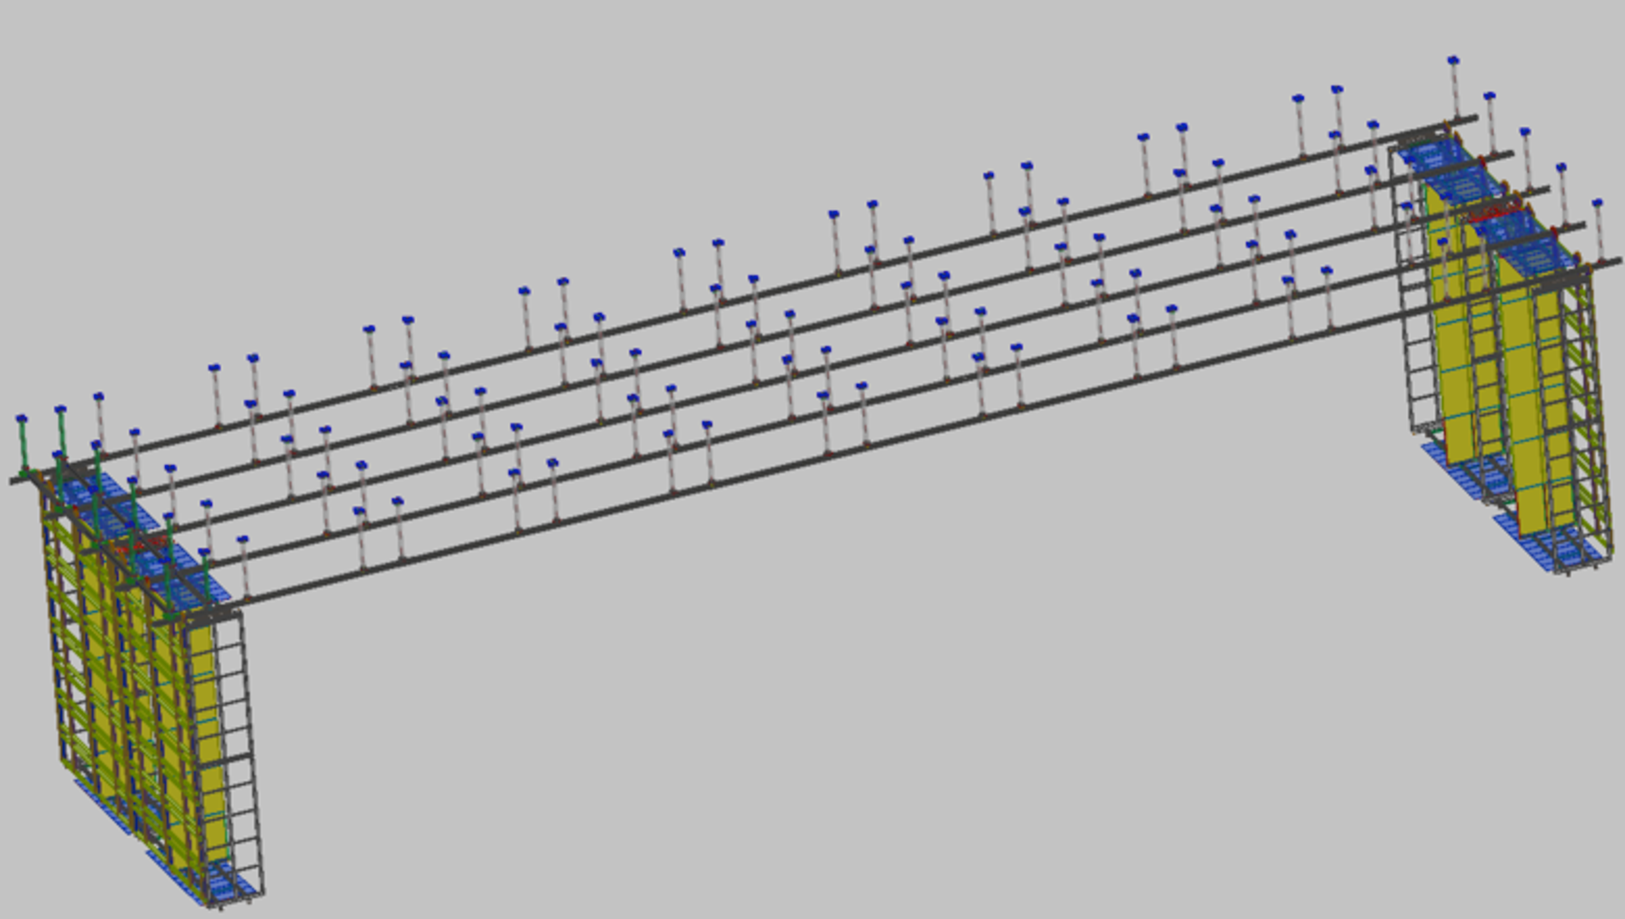
\includegraphics[width=.49\textwidth]{DSS-1.pdf}
 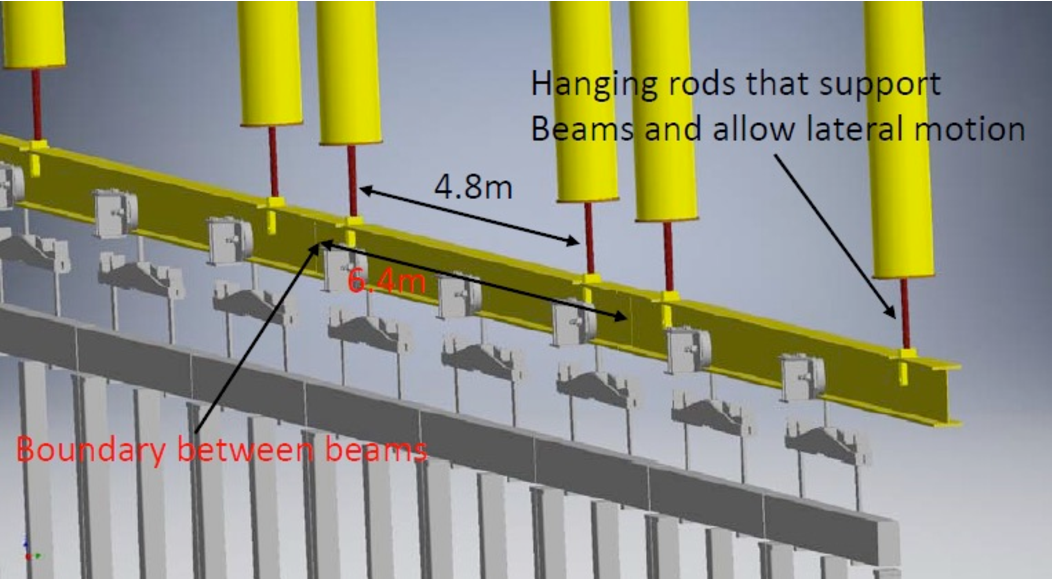
\includegraphics[width=.49\textwidth]{DSS-2.pdf}
\end{dunefigure}


% \textquotedblleft cryostat crossing tubes\textquotedblright\   that penetrate the cryostat insulation.  \ref{fig:crossingtube}


The \dword{dss} is designed to meet the following  requirements:
\begin{itemize}
 \setlength\itemsep{1mm}
\setlength{\parsep}{1mm}
\setlength{\itemsep}{-5mm}
% \small
\item Support the weight of the detector;
\item Accommodate cryostat roof movement during filling, testing, and operation;
\item Accommodate variation in \fdth locations and
  variation in the flange angles due to installation tolerances and
  loading on the warm structure;
\item Accommodate shrinkage of the detector and \dword{dss} from ambient
  temperature to \dword{lar} temperature;
\item Define the positions of the detector components relative to each other; 
\item Provide electrical connection to the cryostat ground and remain electrically isolated from the detector;
\item Allow support penetrations to be purged with gaseous argon to prevent contaminants from diffusing back into the liquid; 
\item Ensure that the instrumentation cabling does not interfere with the \dword{dss};
\item Consist entirely of components that can  
be installed through the \dword{tco};
\item Meet AISC-360 codes. % or appropriate codes required at \dword{surf}; \fixme{and/or?}
\item Meet seismic requirements one mile underground at \dword{surf};
\item Consist entirely of materials compatible %for 
with operation in ultrapure \dword{lar};
\item Ensure that beams are either completely submerged in \dword{lar} or completely in the ullage;  
\item Ensure that detector components are not less than \SI{400}{mm} from the membrane flat surface;
\item Ensure that the supports do not interfere with the cryostat I-beam structures;
\item Ensure that the detector's lower \dword{gp} is lies over the cryogenic piping and that the tops of the \dword{dss} beams are submerged in \dword{lar} while leaving a \SI{4}-\SI{5}{\%} ullage at the top of the cryostat; 
\item Include the infrastructure necessary to move the \dword{apa} and
  \dword{cpa}-\dword{fc} assemblies from outside the cryostat through the
  \dword{tco} and to the correct position.
\end{itemize}

Each row of the \dword{dss} consist of a series of \num{10} \SI{6.4}{m}-long
W10$\times$26 stainless steel I-beam sections for a total of \num{50} I-beam segments for the 5 rows. The length of the beam segments was chosen to be a multiple of the \SI{1.6}{m} pitch of the major cryostat beams which allows the regular placement of the support \fdth across the cryostat roof. With a W10$\times$26 I-beam and \SI{6.4}{m} between the supports the beam deflections due to the loads was kept below 5mm. 
Each I-beam is suspended on both ends by the mechanical \fdth{}s that penetrate the cryostat roof. 
During cool down  each I-beam shrinks while the mechanical supports outside the cryostat remain fixed  causing gaps to form between \dword{apa}s that are adjacent but supported on separate beams.
\dword{apa}s that are supported on the same beam will not have gaps develop because both the beam and \dword{apa} frames are stainless steel so they shrink together.
The gap between two adjacent \dword{dss} beams after cooldown will be \SI{17}{mm} which is considered acceptable. 
Increasing the the beam length beyond \SI{6.4}{m} was not considered as the deformation of the I-beam under load would increase, the gap between \dword{apa} on adjacent beams would increase, and the difficulty of installing the beams would increase.
\fixme{need max deflection number from Vic}


\begin{dunefigure}[DSS vertical support \fdth]{fig:DSS-Support}
  { Drawing of the \dword{dss} vertical support \fdth. The detector load is carried by the \SI{25}{mm} inner support rod. The outer lateral support tube prevents swinging during installation.  The \fdth mounts to the cryostat crossing tube which is an integral part of the cryostat. Not shown here are the short vacuum chambers for the CISC instrumentation which can be found on Figure \ref{fig:CISC-feedthru}.}
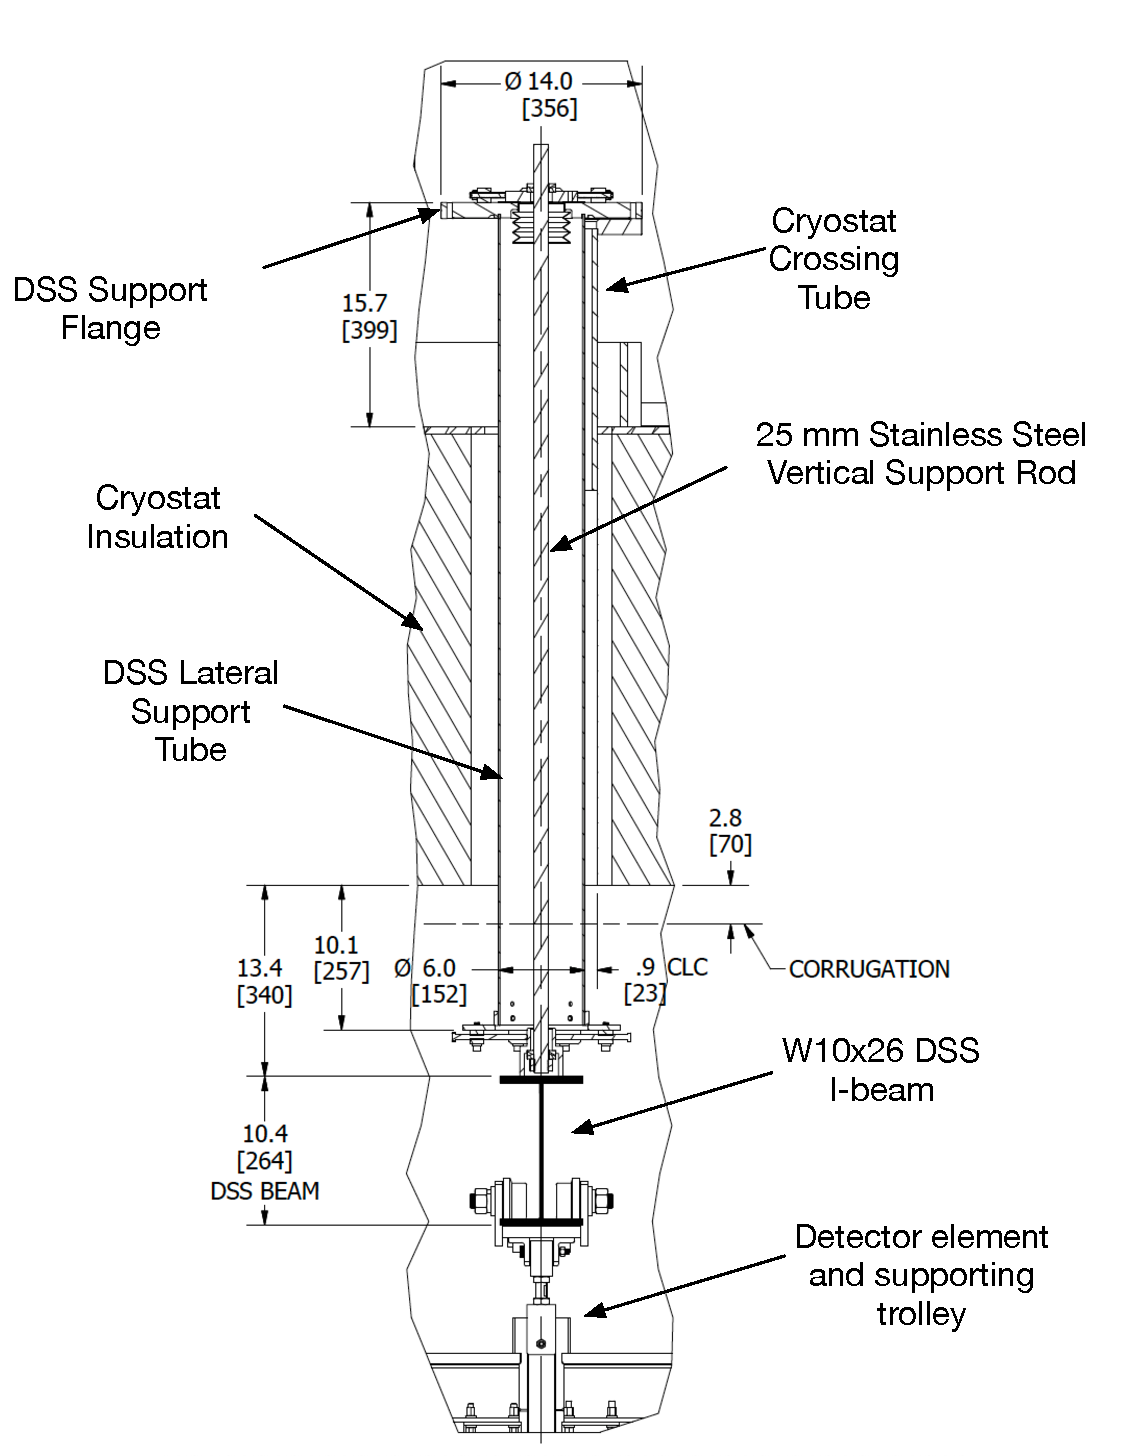
\includegraphics[width=.85\textwidth]{graphics/DSS-Support.pdf}
\end{dunefigure}


The \dword{dss} I-beams are supported on both ends from a vertical support \fdth shown in Figure \ref{fig:DSS-Support}. A \SI{25}{mm} solid stainless steel rod, which is threaded at both ends, runs down the center of the \fdth and carries the detector load. The support  rod connects on the bottom end to a clevis which is then pinned to the \dword{dss} beams shown in Figure \ref{fig:DSS-lateral-support}. At the top the rod bolts to an X-Y table sitting on the top Conflat Flange that allows a lateral adjustment of $\pm$\SI{2.5}{cm} (\SI{1}{in}). A swivel washer is used in the bolted connection to the X-Y table to allow the support rod to swing freely. The bolted connection also allows the \dword{dss} I-beams to be adjusted vertically. The vacuum seal is established at the top with a bellows between the rod and the top flange. The top flange of the \dword{dss} support \fdth is a Conflat flange that connects to the cryostat crossing tube's mating flange. The crossing  tube is welded to the cryostat roof and the top flange is mechanically supported from the cryostat's  \SI{1.1}{m} tall support I-beams. The cryostat crossing tubes are shown in Figure \ref{fig:crossingtube}.

During installation the detector components will be pushed along the \dword{dss} I-beams which will place a lateral load on the \dword{dss} support structure. 
A \SI{15.2}{cm} (\SI{6}{in}) \dword{od}  tube is welded to the top flange of the \dword{dss} \fdth . 
This lateral support tube  extends through the cryostat insulation and has a clamping collar at the bottom which is used to fix the I-beam support clevises in position during installation. 
The bottom of the lateral support tube is seen in Figure \ref{fig:DSS-lateral-support}. 
The long bolts press on the flat sides of the clevis to fix the support rod's location. 
There is a nominal \SI{10}{mm} gap between the OD of the support tube and the \dword{id} of the clearance tube in the cryostat. 
The clevis can be positioned anywhere inside the \SI{15.2}{cm} tube.




\begin{dunefigure}[DSS support for lateral loads ]{fig:DSS-lateral-support}
  {Left panel shows how the central support rod is locked in postion during detector installation. The outer  \SI{15.2}{cm} (\SI{6}{in}) tube is used to fix the support clevis in position. The right panel shows the system as it is connected to the I-Beam.}
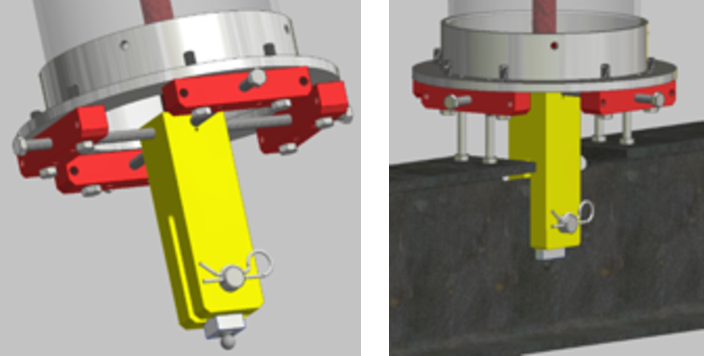
\includegraphics[width=.75\textwidth]{graphics/dss-lateral-support.pdf}
\end{dunefigure}

After the detector has been installed all restraints on the clevis are released to allow motion as the detector contracts during cool down.  The two support rods that support each \dword{dss} beam will contract and move toward each other by 13.1 mm along the axis of the detector.  
The drift distance will shrink by 7.4 mm caused by the contraction of the field cages.  The detector is symmetric in the drift direction around the center \dword{apa}.  The drifts on either side of the center \dword{apa} will  shrink toward the center while the center \dword{apa} remains unmoved.  This results in the \dword{cpa}s moving 7.4 mm toward the center and the outer \dword{apa}s moving 14.8 mm (2$\times$7.4 mm) toward the center.  The hanging rod is designed to have a range of motion of 15 mm in the drift direction to accommodate this shrinkage.




Detector components are installed using a shuttle beam system as
illustrated in Figure~\ref{fig:shuttle}.  
The last two columns of \fdth{}s (western-most) support temporary beams that run
north-south, perpendicular to the main \dword{dss} beams.  
A shuttle beam has trolleys mounted to it and transverses 
north-south until it aligns with the required row of \dword{dss} beams.  
The last \dword{apa} or \dword{cpa} in a row is supported by the shuttle beam, which is bolted directly to the \fdth{}s once it is in place.  
As the last \dword{cpa} or \dword{apa} in each row is installed, the north-south beams are removed.

\begin{dunefigure}[\threed models of the shuttle beam end of the \dword{dss}]{fig:shuttle}
  {\threed models of the shuttle beam end of the \dword{dss}. The figures show how an \dword{apa}
is translated into position using the north-south beams until it lines up with the correct
row of I-beams.}
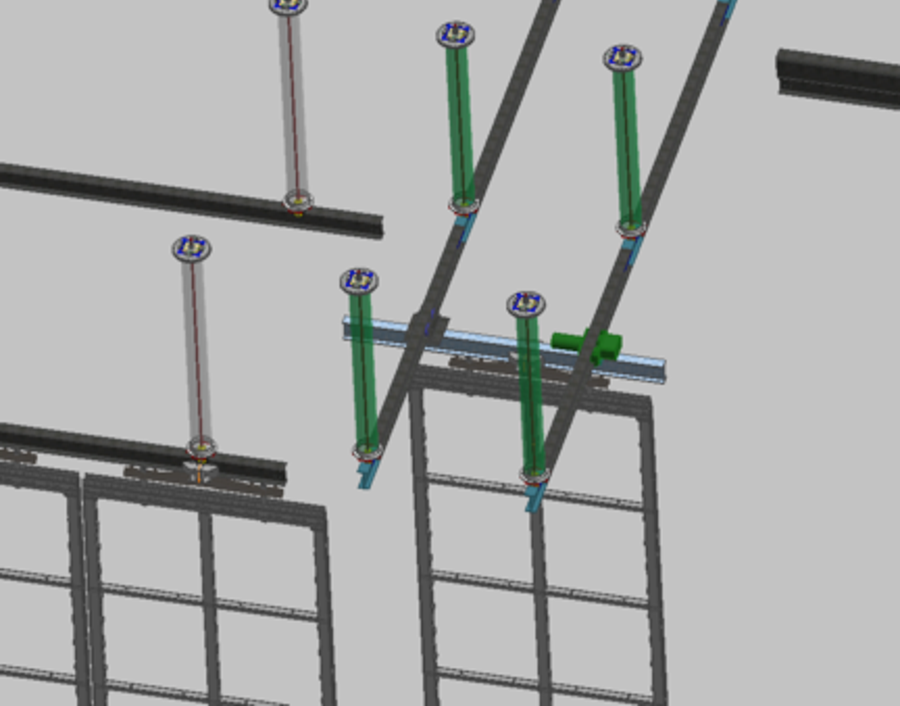
\includegraphics[width=.49\textwidth]{/Shuttle-1.pdf}
 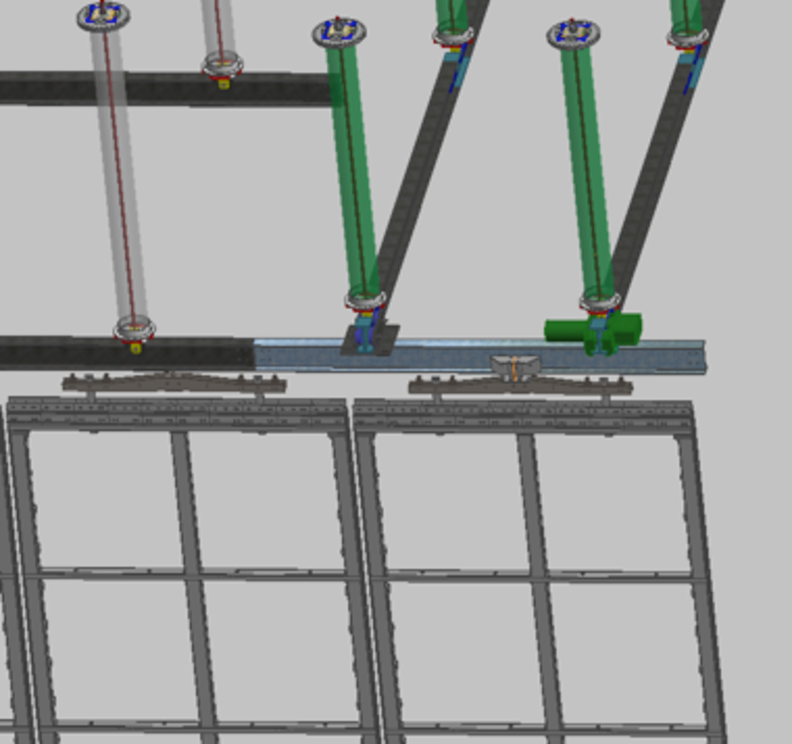
\includegraphics[width=.42\textwidth]{shuttle-2.pdf}
\end{dunefigure}

A mechanical stops  prevents trolleys
from passing the end of the shuttle beam unless it is aligned with a
corresponding \dword{dss} beam.  The shuttle beam and each detector component are
moved using a motorized trolley.  A commercially available motorized
trolley will be modified as needed for the
installation. 




\begin{dunefigure}[Prototype of the motorized DSS trolley ]{fig:DSS-trolley}
  {Prototype of the motorized DSS trolley that will push the APA and CPA along the I-beams and through the switchyard.}
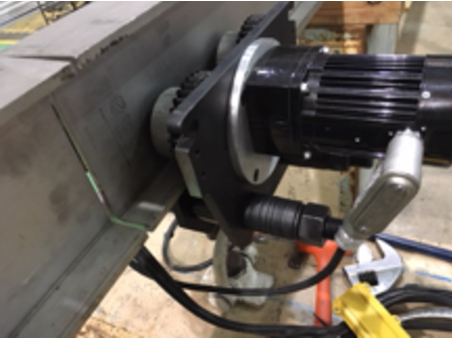
\includegraphics[width=.49\textwidth]{graphics/DSS-trolley.pdf}
\end{dunefigure}



A mock-up of the shuttle system will be constructed to test the
mechanical interlock and drive systems for the shuttle beam
for each \dword{detmodule}.  Tests will be conducted to evaluate the level of
misalignment between beams that can be tolerated and the amount of
positional control that can be achieved with the motorized trolley. We plan to construct a full scale prototype of a section of the  switchyard and perform tests at floor level. Later, the test program will be expanded at Ash River, where a full scale installation test will be performed. This is described in 
Section~\ref{sec:fdsp-tc-infr-qaqc}.


%%%%%%%%%%%%%%%%%%%%%%%%%%%%
\subsection{Cryostat Roof Infrastructure}
\label{sec:fdsp-tc-infr-cryo-roof}

\fixme{Flooring, Racks, Cooling, cable trays, Crossing tubes, GAr}
%%%%%%%%%%%%%%%%%%%%%%%%%%%%
\subsection{Cryostat Internal}
\label{sec:fdsp-tc-infr-cryo-int}

\fixme{Flooring, Lighting, Access equipment}

%%%%%%%%%%%%%%%%%%%%%%%%%%%%
\subsection{Cleanroom/airlock Infrastructure}
\label{sec:fdsp-tc-infr-comm}

\begin{dunefigure}[APA assembly tower]{fig:apa-assemble-frame}
  {Image of the \dword{apa} assembly tower with the \dword{apa} assembly frame attached. The transport rails at the top of the figure are used to move the assembled \dword{apa} into the cleanroom. The work decks allow access to the \dword{apa} from multiple levels. }
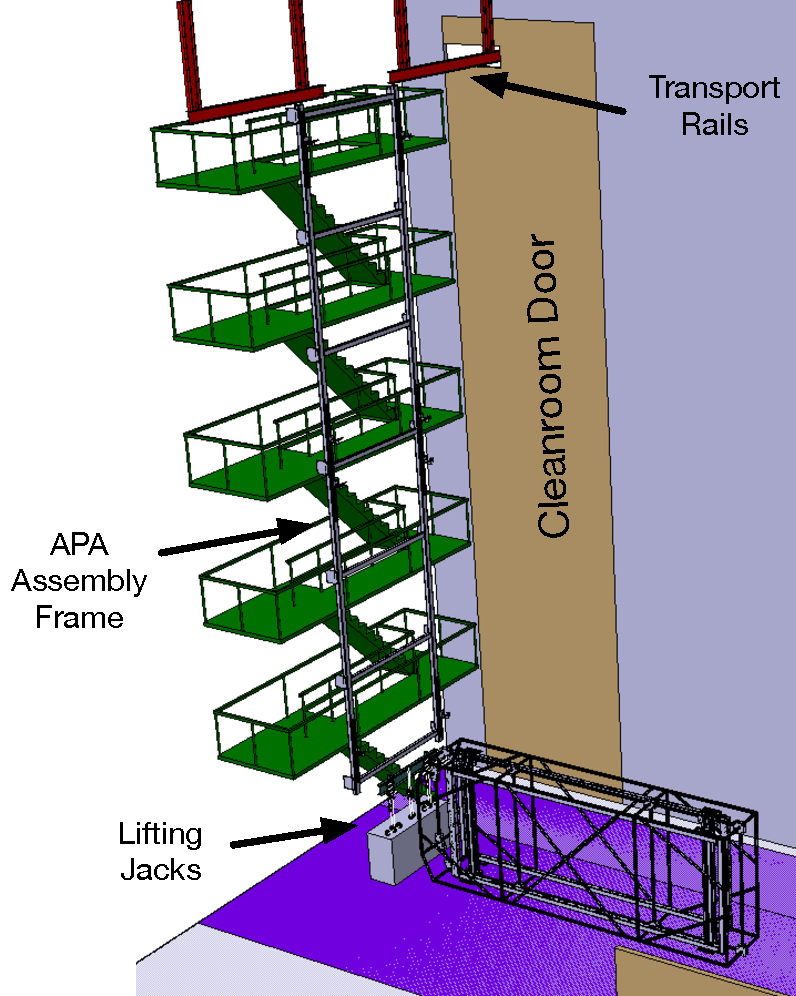
\includegraphics[width=.9\textwidth]{apa-assemble-frame}
\end{dunefigure}


\begin{dunefigure}[APA cabling tower]{fig:apa-cable-tower}
  {Image of the \dword{apa} cabling tower. The two reels of cable for the electronics are shown. The work decks allow access to the \dword{apa} from multiple levels. }
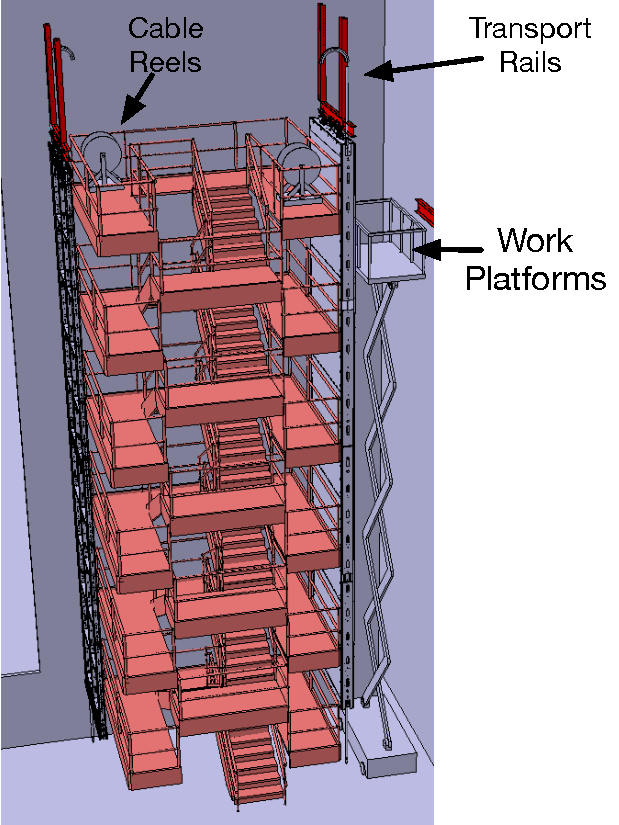
\includegraphics[width=.9\textwidth]{apa-cable-tower}
\end{dunefigure}



%%%%%%%%%%%%%%%%%%%%%%%%%%%%
\subsection{Prototyping and Testing (QA/QC)}
\label{sec:fdsp-tc-infr-qaqc}

\fixme{QA/QC Prototyping and testing}

%%%%%%%%%%%%%%%%%%%%%%%%%%%%
\subsection{Safety}
\label{sec:fdsp-tc-infr-safety}


%%%%%%%%%%%%%%%%%%%%%%%%%%%%
\subsection{Costs, Schedule and Risk Analysis}
\label{sec:fdsp-tc-infr-cost}

\fixme{use templates from cost-risk-sched.tex file. Anne}


% Note: infrastructure.tex inputs dss.tex



%%%%%%%%%%%%%%%%%%%%%%%%%%%%%%%%%%%%%%%%%%%%%%%%%%%%%%%%%%%%%%%%%%%%
%\section{Detector Installation}
%\label{sec:fdsp-tc-inst}

\section{Detector Installation}
\label{sec:fdsp-tc-inst}


%The \dword{dune} detector installation will proceed in three phases: the \dword{cuc} set up, the installation set up, and the detector installation. Figure \ref{fig:high-level-schedule} shows the major underground activities and gives an idea of what work will be occurring in which phase. \dword{cuc} set up is the first step in the installation process. The phase begins when the underground area for the north cavern and central cavern become available to \dword{lbnf} and \dword{dune}. At this time, the cryostat construction can begin in the north cavern, and \dword{dune} equipment installation can begin in the central cavern or \dword{cuc}. Figure~\ref{fig:cavern-layout} shows a top view of the underground areas. The equipment from \dword{dune} installed in this phase is the infrastructure in the \dword{dune} dataroom. Figure~\ref{fig:cavern-layout} shows he dataroom in the \dword{cuc} on the west end of the excavation. The detector installation setup phase (referred to as Infrastructure Det\#1 in Figure \ref{fig:cavern-layout}) begins during the cryostat membrane installation period. In this phase, the equipment needed for detector installation will be erected in north cavern. This includes installing the bridge across the cavern, the cleanroom, lifting equipment and work platforms, the coldboxes, and the cryogenic system for testing \dword{apa}, and the \dword{dss} with the related switchyard. In the third phase of the installation, the detector itself will be installed. The work in each phase will be described the following sections.


\begin{dunefigure}[High level installation  schedule]{fig:high-level-schedule}
  {Overview schedule showing the main activities underground.
  \fixme{need update from bill}}
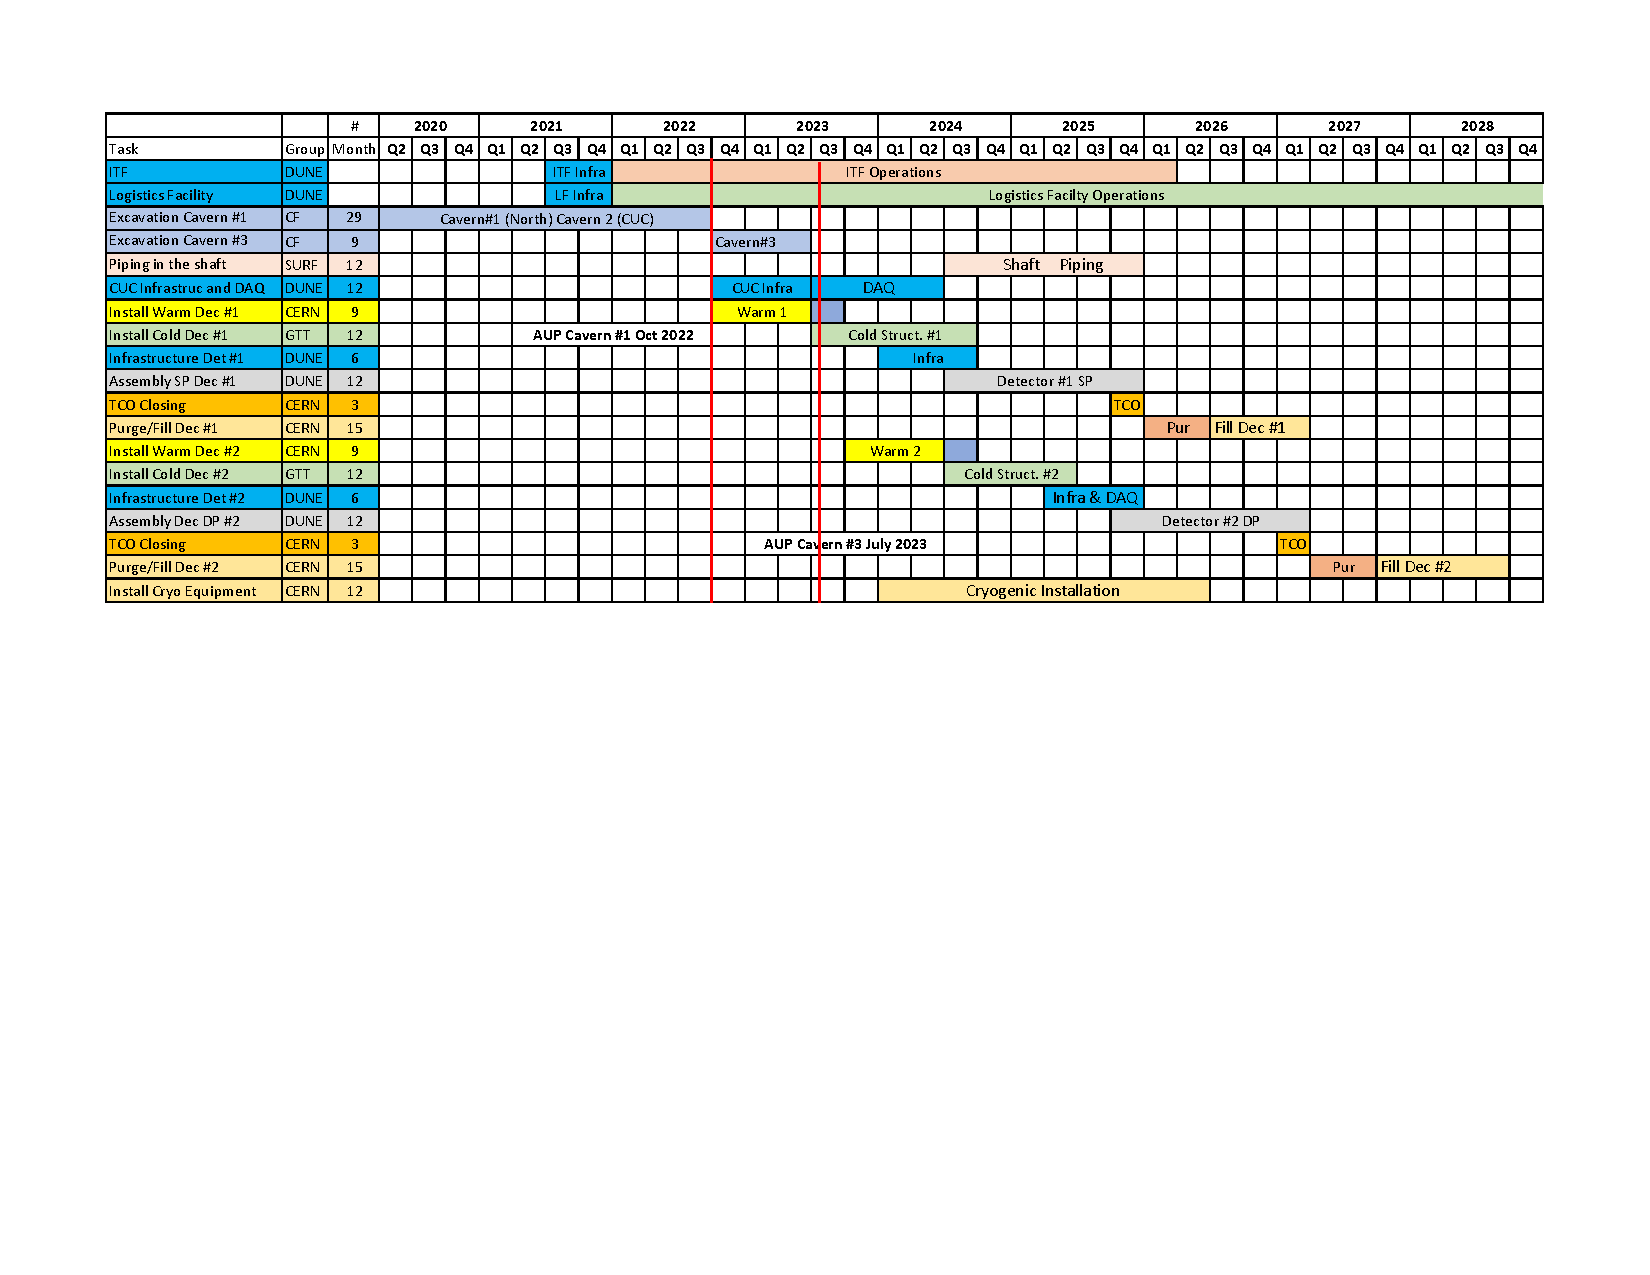
\includegraphics[width=.99\textwidth]{high-level-schedule}
\end{dunefigure}



As mentioned in Section~\ref{sec:fdsp-tc-log}, the \dword{dune} detector installation will proceed in three phases: \dword{cuc} set up, installation set up, and the detector installation. Figure \ref{fig:high-level-schedule} shows the major underground activities and gives an idea of what work occurs in each phase. 

\dword{cuc} set up is the first step in the installation process. This phase begins when the underground area for the north cavern and central cavern become available to \dword{lbnf} and \dword{dune}. At this time, the \dword{lbnf} cryostat construction can begin in the north cavern, and \dword{dune} equipment installation can begin in the \dword{cuc}. Figure~\ref{fig:cavern-layout} shows a top view of the underground areas. The \dword{dune} equipment  installed in this phase is the infrastructure in the \dword{dune} dataroom. Figure~\ref{fig:cavern-layout} shows the dataroom in the \dword{cuc} on the west end of the excavation. 

The detector installation setup phase (referred to as Infrastructure Det\#1 in Figure \ref{fig:high-level-schedule}) begins during the cryostat membrane installation period. In this phase, the equipment needed for detector installation is erected in the north cavern. This includes the bridge across the cavern, the cleanroom, lifting equipment and work platforms, the \coldbox{}es, and the cryogenics system for \dword{apa} testing, and the \dword{dss} and switchyard. 

The detector itself is installed in the third phase of the installation. 

\begin{dunefigure}[Layout of the DUNE underground areas]{fig:cavern-layout}
  {Top view of the layout at the 4850 level at SURF. Shown are the three large excavations and the location of detectors in excavations \#1 and \#3. Excavation \#2 is the CUC, which houses the DUNE dataroom and the underground utilities.}
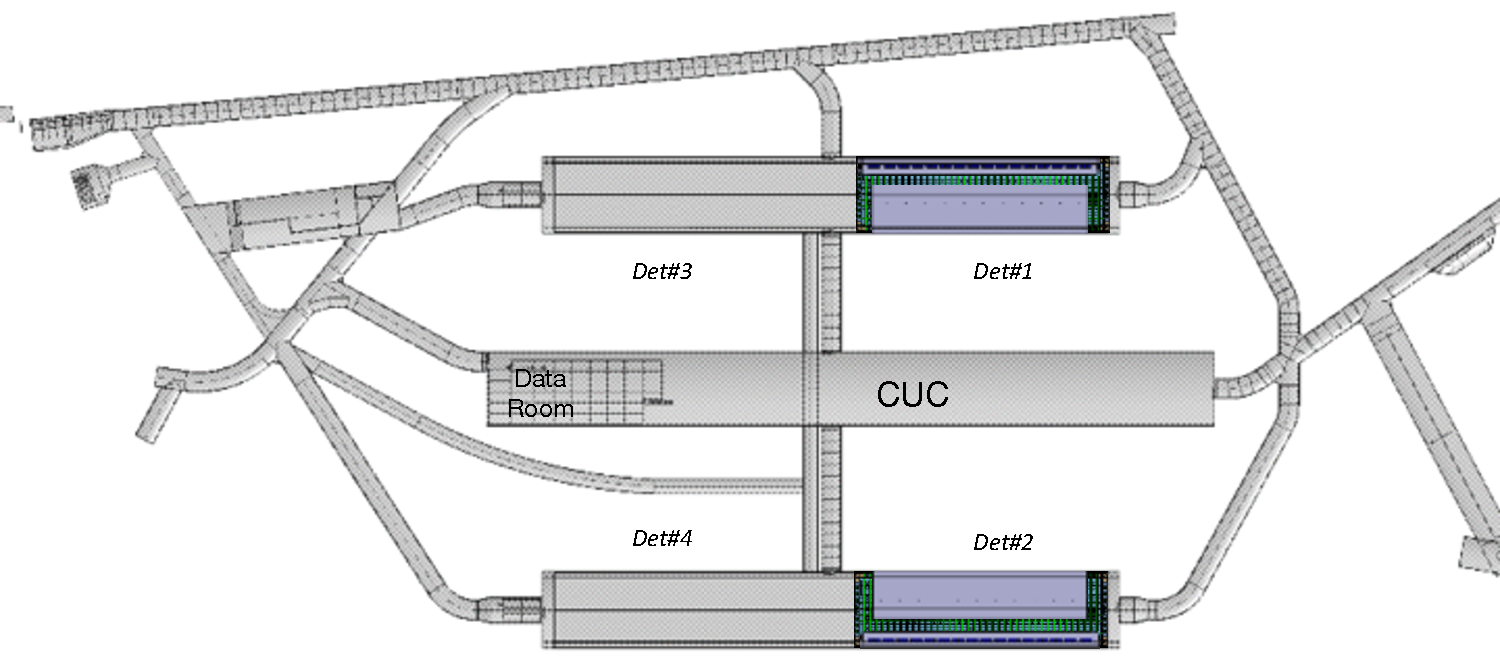
\includegraphics[width=.9\textwidth]{cavern-layout}
\end{dunefigure}


%%%%%%%%%%%%%%%%%%%%%%%%%%%%
\subsection{Installation Process Description}
\label{sec:fdsp-tc-inst-proc}


\subsubsection{CUC Installation Phase}
\label{sec:fdsp-tc-inst-CUC}

\begin{dunefigure}[Layout of the DUNE data room and work area in CUC]{fig:install-cuc}
  {Top: The overall layout of the \dword{dune} spaces in the \dword{cuc}. A110 is the DUNE data room, which houses the underground computing, and A111 is a general purpose work area (not a control room as labeled) that we call the experimental work area. Bottom: The first row of ten racks in the data room is shown. The first two represent the \dword{cf} interface racks. The images were taken from the ARUP 90\% design drawings U1-FD-A-108 and U1-FD-T-701.}
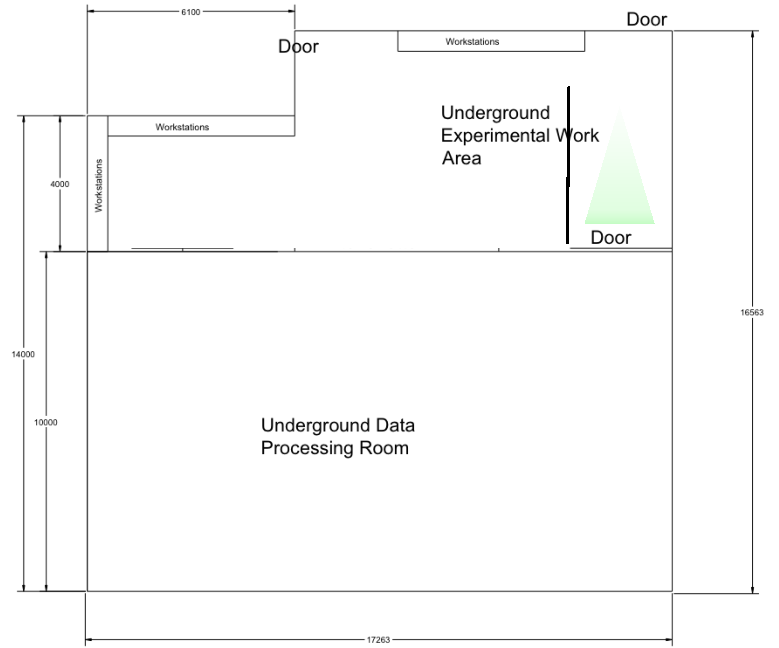
\includegraphics[width=.85\textwidth]{cuc-layout}
\vspace{-2pt}
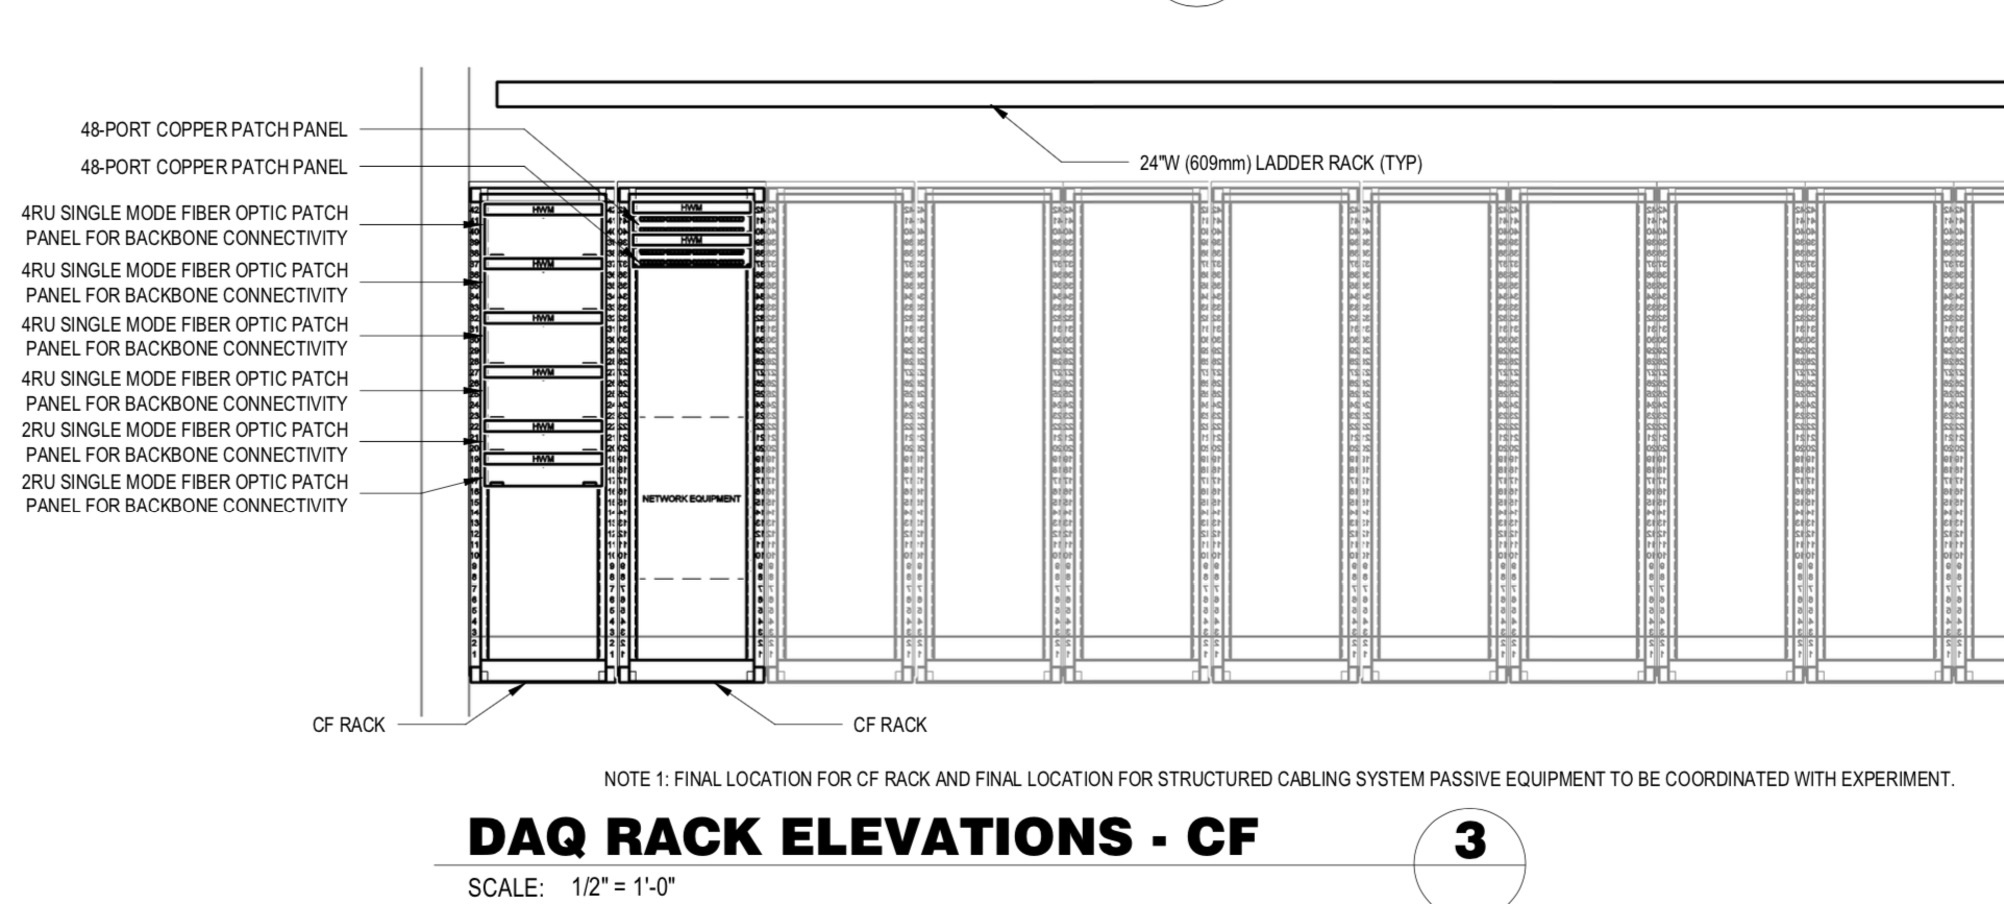
\includegraphics[width=.9\textwidth]{cuc-cf-racks}
\end{dunefigure}

 
Once the \dword{lbnf} \dword{cf} outfitting of the north cavern and the \dword{cuc} is complete,  \dword{lbnf} begins the first cryostat installation in the north cavern and \dword{dune} can begin to install equipment in the dataroom and work area room in the \dword{cuc}. See Figure~\ref{fig:install-cuc}.  \dword{dune} will not have access to the north cavern due to the heavy steel work for the cryostat. 
At this point \dword{lbnf}  \dword{cf} will have installed redundant single-mode fiber up the shafts to provide external connectivity, and in the empty dataroom,  an \SI{18}{in} false floor, a \SI{500}{kVA} power disconnect, and connections for sufficient chilled water to cool the racks. The dataroom, like the adjacent \dword{cf} electronics room, will be outfitted with a dry fire extinguishing system. 
 

The water-cooled racks, cable trays, power distribution, and water distribution in the dataroom are the responsibility of \dword{dune} and will be installed once the space becomes available.  
Installation of the racks must be coordinated with \dword{cf} 
since the first two racks are for \dword{cf} use and must be in place before the first phase of work underground is complete. 
Some small overlap will be needed between \dword{cf} and \dword{dune} at this time. The general purpose network will be installed by \dword{fnal}'s \dword{sdsd} and connected to the shaft fiber. 
This is required for most subsequent work in the underground area.
The \dword{daq} fiber trunk between the detector cavern and the \dword{cuc} dataroom will be installed after the cable trays, electronics mezzanine, and racks are available in the north cavern.


Data from the detector electronics will be transmitted over a multimode fiber trunk from the \dwords{wib} on top the \dword{spmod} to the \dword{daq} data room in the \dword{cuc}, shown in Figure~\ref{fig:install-cuc}.  The data room will contain 60 water-cooled racks, two of which are reserved for \dword{cf} use, two for \dword{cisc} servers, and the rest for \dword{daq} servers and networking. Racks for all four modules will be installed at the beginning of the \dword{cuc} commissioning phase because they must be plumbed into the cooling water below the dataroom's drop floor and wired into power distribution from the ceiling.  \dword{daq} equipment will populate the racks as needed for servicing the detector commissioning.  For the first detector module, details of this configuration will be informed by \dword{daq} vertical slice tests done at other institutions.  

At the same time, the eight above-ground \dword{daq} racks that receive data from the underground data room and  transmit the data to \dword{fnal} will %also 
be installed, connected to the WAN, and connected to the single-mode fiber in the Ross and Yates Shafts.  With this infrastructure in place, the \dword{daq} group can begin constructing and testing the final \dword{dune} \dword{daq}, starting with the %.  The 
timing system. % is the first \dword{daq} component needed.  
Enough \dword{daq} back-end servers to support the first \dword{apa}s will be operational before the \dword{apa}s are installed.  The remainder of the \dword{daq} will grow in parallel with \dword{apa} installation.

The underground experimental work area (shown as ``CONTROL ROOM'' in Figure~\ref{fig:install-cuc}) must serve a variety of purposes during the \dword{dune} installation. Initially, the area will be outfitted with office equipment for the installation team, workstations for \dword{daq}, and a basic conference area for meetings. The room is 17 \si{m} wide with portions that are \SI{5.5}{m} and \SI{8}{m} deep.

During this early installation stage, the machine shop and \dword{dune} storage area will be set up in the detector excavation area and shared with the cryostat team. 

\subsubsection{Installation Setup Phase}
\label{sec:fdsp-tc-inst-setup}

\begin{dunefigure}[Top view of the installation area highlighting the infrastructure]{fig:install-infrastructure-top}
  {Top view of the installation area highlighting the infrastructure. The cleanroom roof and cavern walls are removed in this view.}
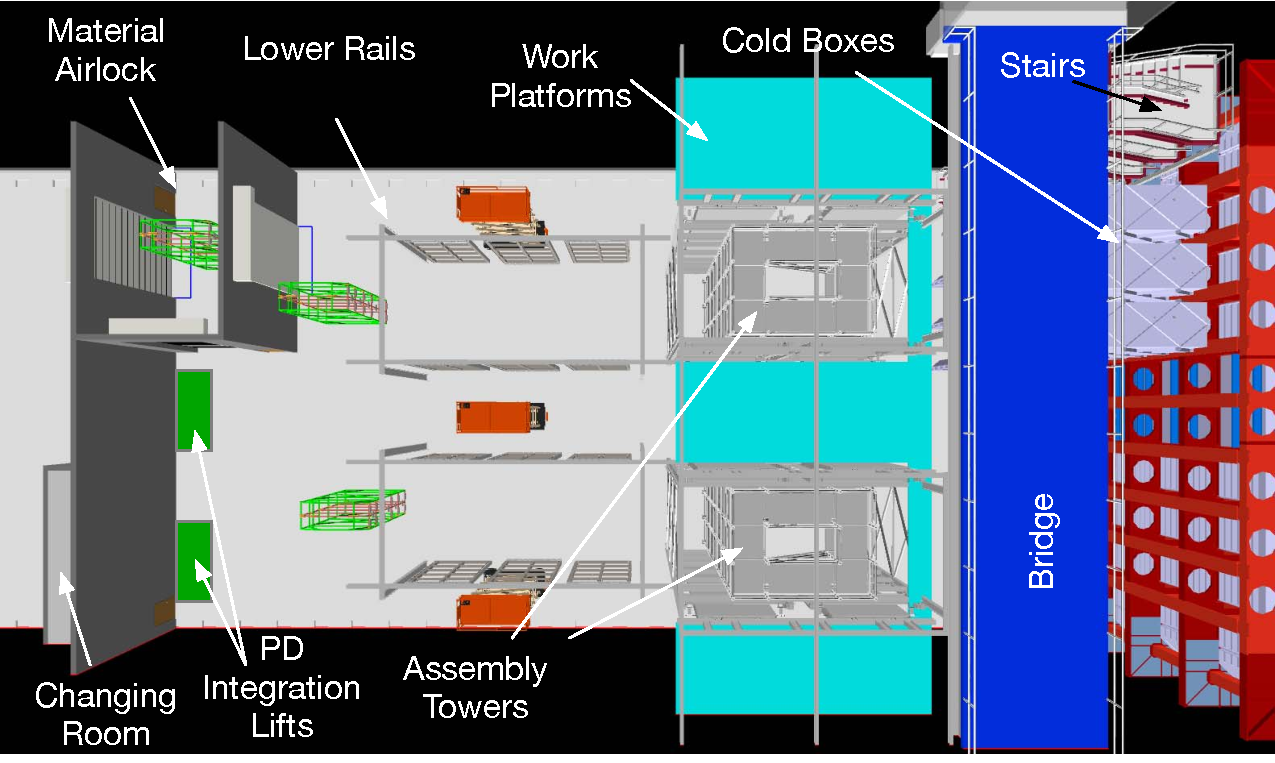
\includegraphics[width=.95\textwidth]{install-infrastructure-top}
\end{dunefigure}

Once the steel structure of the cryostat is complete, the remaining work by the \dword{lbnf} cryostat team will be focused inside the cryostat installing the insulation and membrane.  
\dword{lbnf} activity outside the cryostat will consist mainly of
transporting the 4,000 crates of foam and other materials from the cavern to inside the cryostat. 
Since the cryostat outer steel structure will be in position, \dword{dune} can 
begin installing the infrastructure needed to install the detector. 
Figure \ref{fig:install-infrastructure-top} shows the major pieces of infrastructure supporting the detector installation.
The first piece of equipment, the bridge between the north and south drifts. 
This will allow the cryogenics equipment to travel from the north drift to the \dword{cuc} and will provide part of the structure for the cleanroom. It also provides an additional means of egress in an emergency.

As part of the bridge construction the crane under the bridge will also be mounted. This can then be used to lift crates off the floor and bring them into the cryostat. This frees the cavern crane for work elsewhere.

The largest, most and most time consuming piece of equipment to be constructed in this phase are the three \coldbox{}es and the associated cryogenics system. 
The \coldbox{}es, visible in Figure \ref{fig:install-coldbox} and \ref{fig:install-infrastructure-top}, must be constructed in place due to their size. Because of the time needed for their construction fabrication needs to begin as early as possible. As part of the further engineering design it will be investigated if the \coldbox{}ex  can be constructed in pieces above ground, transported underground and assembled. If possible this will also make moving the \coldbox{}es to the second detector possible. 
 
After the bridge crane is installed the \dword{apa} assembly and cabling towers can be installed. 
The two towers have a wide aisleway between them so they will not impede the cryostat fabrication. 
With the towers in place the north-south support beams and the fixed platforms can be installed. 
This work is done at height so it will only cause temporary interruptions to the material transport along the floor.

The lower set of rails and the \dword{cpa} assembly equipment be installed at the convenience of the cryostat installation crew.

When the cryostat membrane work is complete the cryogenic piping inside the cryostat can be installed, the cryostat cleaned and the false floor installed. After the cryostat is cleaned the filters will be installed in air handling units for the cryostat and purified air will begin flowing. A curtain over the TCO can be used to prevent dust from the cavern from entering the cryostat.

In parallel to the installation of the cryogenic piping the walls of the cleanroom can be assembled, the floor painted and the fixed lifts installed. Finally the fixed lighting, AC power, and fire suppression systems are installed in the cleanroom and then it is cleaned and is ready for operation.



On the cryostat roof the installation of the cryostat crossing tubes will follow the cryostat assembly sequence.  \fixme{add LBNF TDR reference. } 
The crossing tubes are welded to the \SI{1}{cm} thick steel cryostat roof and cross braced to the large I-Beams. 
The thin-walled tubes that penetrate the foam insulation are welded to the cryostat inner membrane.


\begin{comment}
Most of the cryostat installation work takes place inside the cryostat and at the bottom (4910 level). 
Thus the cryostat roof is available to the \dword{lbnf} and \dword{dune} installation teams to complete much of the work for installing the cyrogenics system and setting up for the detector installation.  
\end{comment}

\begin{dunefigure}[Installation of electronics crosses]{fig:install-elect-cross}
  {Installation of the crosses to which the \dword{ce} warm readout and the \dword{pd} cables are connected.}
 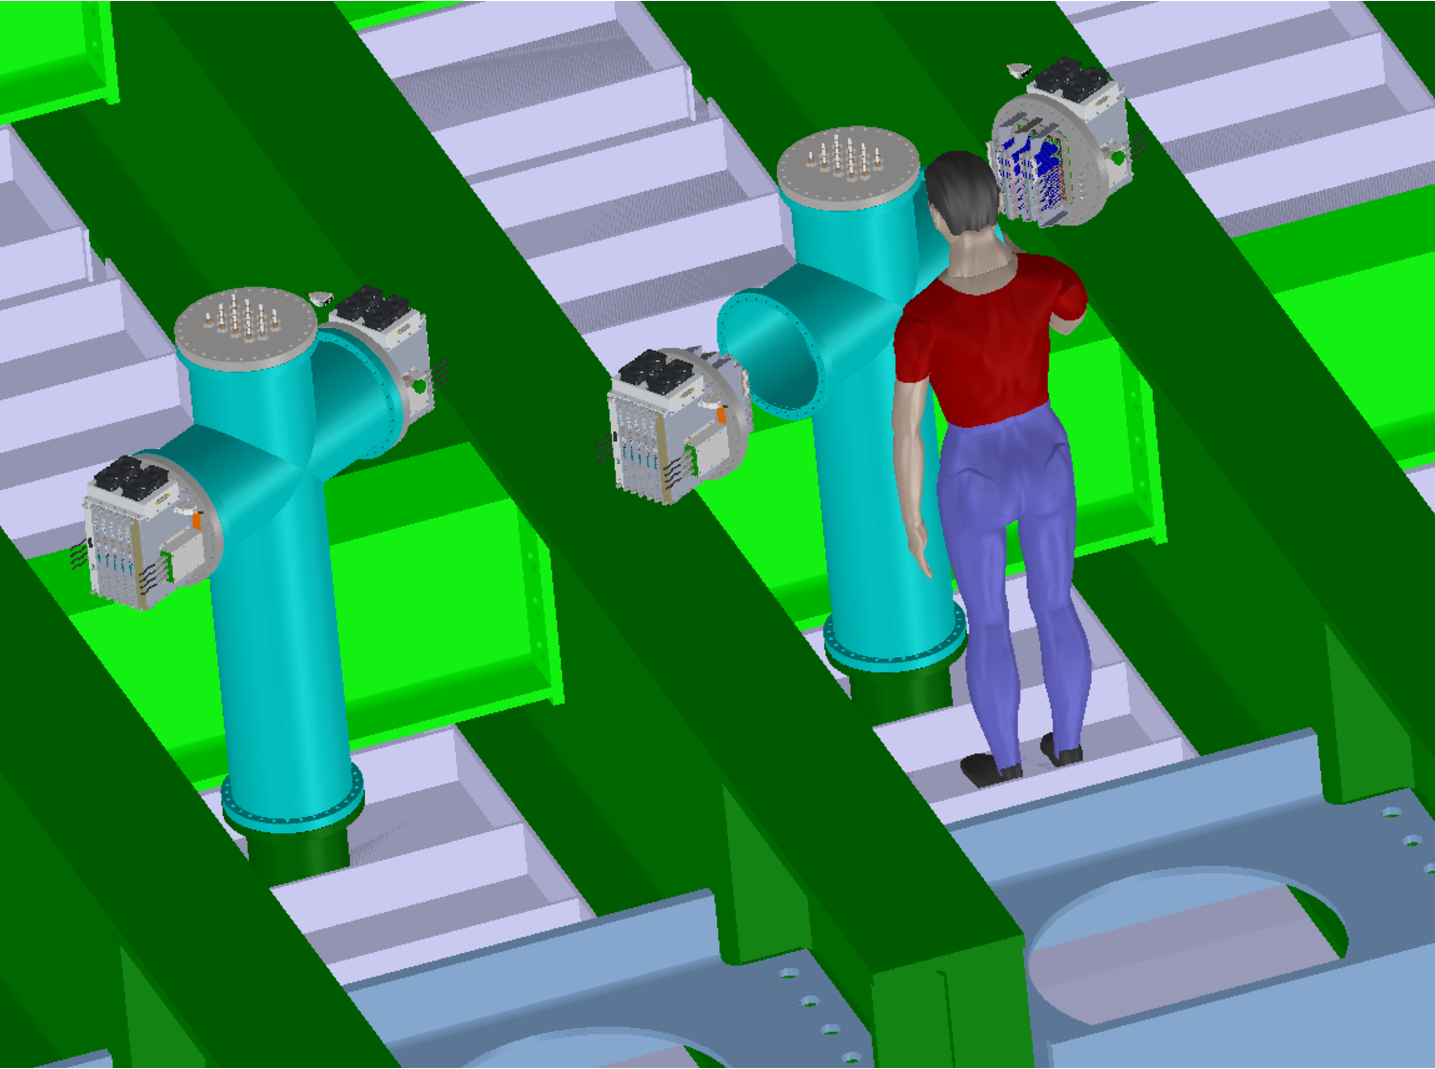
\includegraphics[width=.75\textwidth]{install-elect-cross}
\end{dunefigure}



Once the crossing tubes are installed and leak chased, 
we connect the  \dword{ce} crosses and mount  the feedthrough flanges for the \dword{ce} and \dwords{pd} onto the crosses. 
The height of the crosses was chosen to allow a person to work comfortably on the \dwords{wec}  and \dword{pd} flanges while standing on the cryostat roof. 
A fully assembled cross is shown on the left of Figure~\ref{fig:install-elect-cross}, and a cross with a \dword{wec} extracted in ``assembly position'' is shown on the right. 
The present plan is to install the crosses shortly after the cryostat crossing tubes are installed. 
This allows us to seal the large openings in the cryostat roof to prevent dust from entering.
For this stage, temporary seals are used for the flanges because they must be removed during the cabling process later in the installation. 
When the \dword{wec} installation is complete the \dword{ce} is ready for the installation of power and fiber optics for readout. 

\begin{dunefigure}[DSS \fdth  installation]{fig:install-dss-feedthru}
  {The \dword{dss} support \fdth{}s  are installed using a gantry crane running along the roof of the cryostat. The cryostat decking is not shown 
  so the gantry can move freely on the cryostat roof decking. The gantry crane is selected to fit under the mezzanine as shown in the right panel.}
  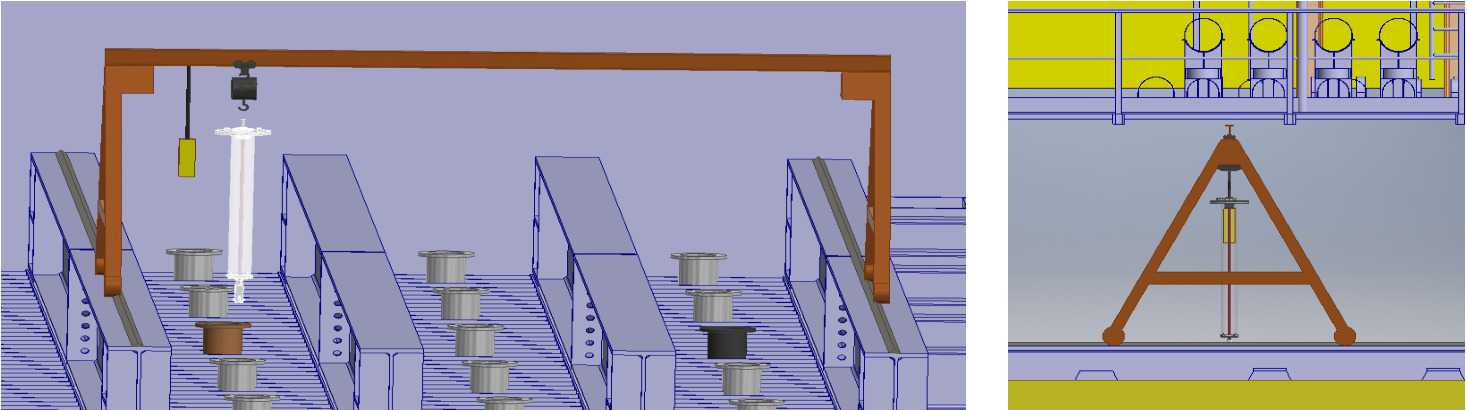
\includegraphics[width=.98\textwidth]{graphics/install-dss-feedthru-v2.pdf}
 %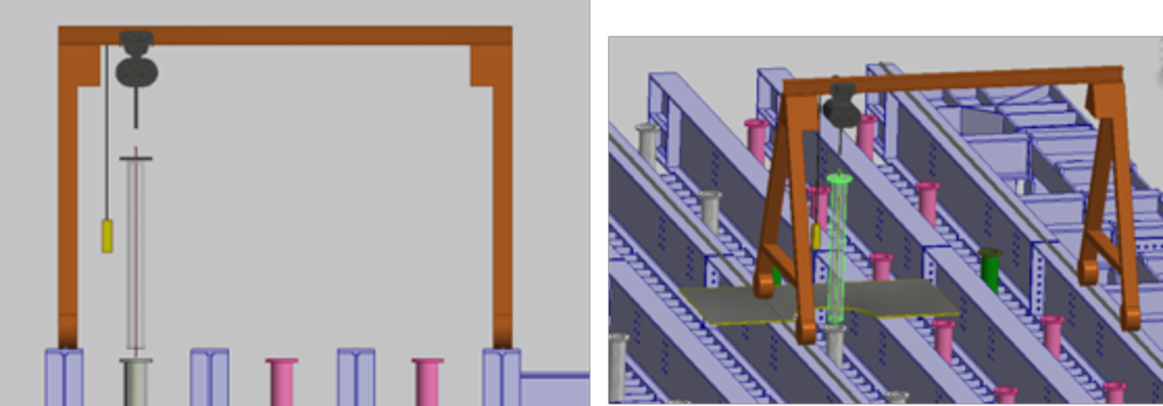
\includegraphics[width=.95\textwidth]{graphics/dss-feedthru-install.pdf}
\end{dunefigure}


The \dword{dss} support \fdth{}s can be installed in parallel to the \dword{ce} crosses. This is the first step in the \dword{dss} installation. 
A gantry crane on top of the cryostat picks up the \fdth{}s  and lowers them into the cryostat crossing tubes as shown in Figure \ref{fig:install-dss-feedthru}. 
There are \num{20} \fdth{}s per row and five rows, for a total of \num{100} \fdth{}s.  A fixture with a tooling ball is attached to the clevis of each \fdth{}.  
The horizontal $xy$ and the vertical $z$ positions of this tooling ball are defined, survey is performed to determine the location of each tooling ball center, and adjustments are made to get the tooling ball centers to within $\pm$\SI{3}{mm} of the nominal location.  
The \SI{6.4}{m} long I-beams are then raised and pinned to the clevis.  
Each beam weighs roughly \SI{160}{kg} (\SI{350}{lbs}). 
A lifting tripod is placed over each  \fdth{}'s supporting beam, and a \SI{0.64}{cm} (\SI{0.25}{in})  cable is fed through the top flange of the \fdth down \SI{14}{m} to the cryostat floor where it is attached to the I-beam. 
The cable access port and lifting cable are shown in Figure \ref{fig:dss-beam-lifting}. 
The winches on each tripod raise the beam in unison to position it at the correct height for pinning to the \fdth clevis.  Once the beams are mounted, a final survey of the beams ensures proper placement and alignment. 
 \begin{dunefigure}[DSS I-Beam lifting setup]{fig:dss-beam-lifting}
  {A cable access port is included in the \dword{dss} flange. This is used to feed a cable from the roof through the flange and attach it to the I-beams during \dword{dss} installation.}
 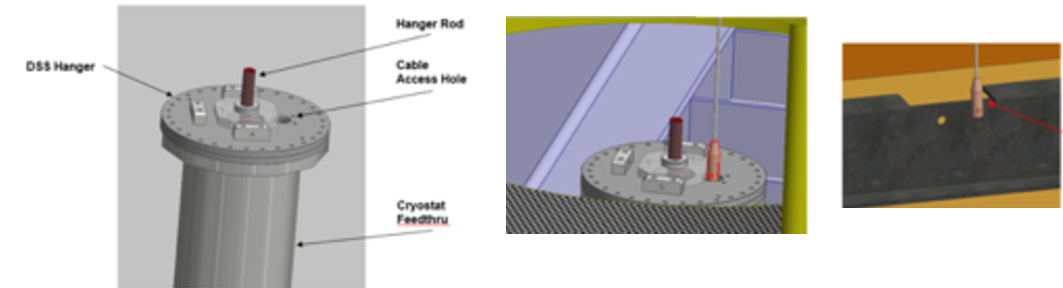
\includegraphics[width=.95\textwidth]{graphics/dss-beam-lifting.pdf}
\end{dunefigure}


Next it is time to install the mezzanines for the cryogenics system and the detector electronics racks, followed by installation of the cable trays,  piping, lighting, and cryostat roof flooring. At this point, the cryostat roof is ready for \dword{daq} installation to begin; this will proceed in parallel to the detector installation.

\fixme{when does the flooring on the cryostat roof get installed?}



\subsubsection{Detector Installation Phase}
\label{sec:fdsp-tc-inst-execute}

\begin{comment}
\begin{dunefigure}[Top view of the installation region inside the cleanroom ]{fig:install-cleanroom-layout}
  {Top view of the cleanroom used for installation. In this view, cleanroom roof and bridge are not shown. The equipment used for installation is shown along with the material airlock layout and the location of the changing room. The cryostat is to the right of the figure and the I-beams passing through the TCO opening are shown.}
 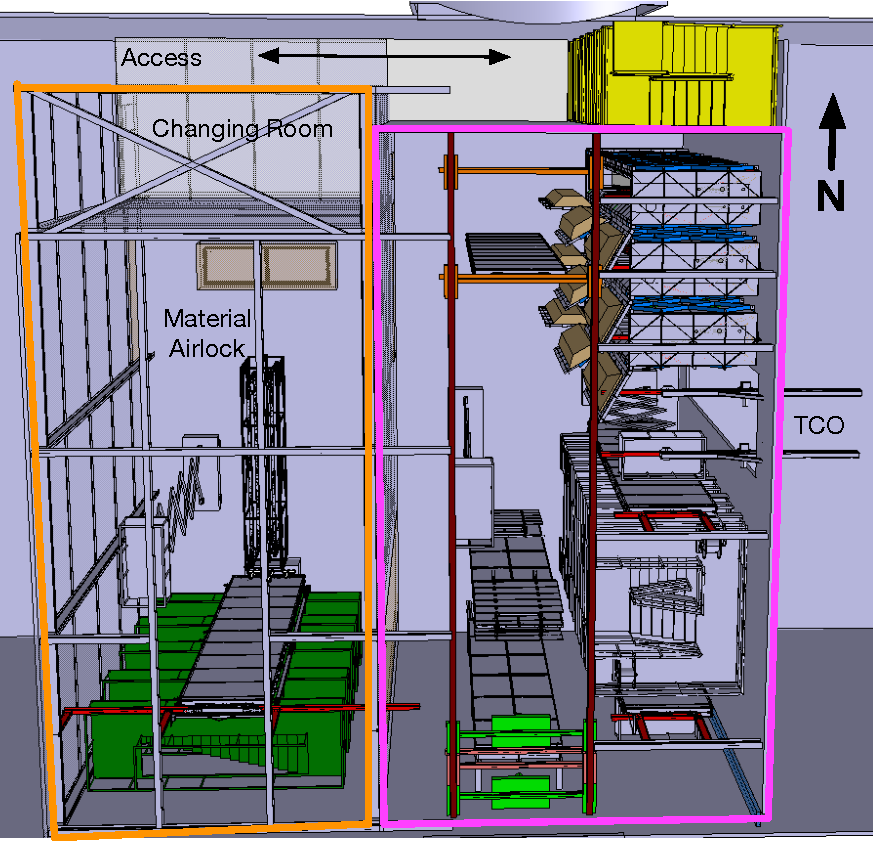
\includegraphics[width=\textwidth]{install-cleanroom-layout}
\end{dunefigure}
\end{comment}

\begin{comment}
The plan is to bring all detector elements into the cleanroom through large roll up doors in the side wall of the airlock. The materials will be moved using using  a battery operated forklift and electric pallet jacks. The airlock will be  13 \si{m} wide 10 \si{m} deep and 17 \si{m} tall. This is large enough to hold the \dword{apa} assembly tower described below with enough extra space to move large objects inside. An access hatch is planned for the roof, allowing the cavern bridge crane to be used in the central area of the airlock. The crane is needed to manipulate the \dword{apa} modules in the airlock. %; the plan calls for assembly of the double-high \dword{apa} pairs there. 



Cabling of the \dword{apa}, cold testing of the \dword{apa}, and assembly of the cathode \dword{fc} modules will take place here. The tower for the \dword{apa} cabling, the \coldbox{}es for testing, and the switchyard for moving the 12m tall objects are described below. All areas of the airlock and cleanroom will be outfitted with UV filtered lights. In addition to this cleanroom, the inside of the cryostat will also be effectively a cleanroom.  By filtering the air and forcing it  into the cryostat at the east end, the clean air will flow through the cryostat and out through the cleanroom and airlock. This will keep the inside of the cryostat at least at ISO-8. The construction process for the cleanroom is still at the conceptual level so what is shown is a steel frame structure where panels can be mounted. %The size is substantial and the occupancy significant, so the cleanroom should have electrical outlets, UV filtered lighting, and fire protection. 
Given the substantial size and the significant occupancy, the cleanroom will have electrical outlets, UV filtered lighting, and fire protection. 


Cabling of the \dword{apa}, cold testing of the \dword{apa}, and assembly of the cathode \dword{fc} modules will take place here. The tower for the \dword{apa} cabling, the \coldbox{}es for testing, and the switchyard for moving the 12m tall objects are described below. All areas of the airlock and cleanroom will be outfitted with UV filtered lights. In addition to this cleanroom, the inside of the cryostat will also be effectively a cleanroom.  By filtering the air and forcing it  into the cryostat at the east end, the clean air will flow through the cryostat and out through the cleanroom and airlock. This will keep the inside of the cryostat at least at ISO-8. The construction process for the cleanroom is still at the conceptual level so what is shown is a steel frame structure where panels can be mounted. %The size is substantial and the occupancy significant, so the cleanroom should have electrical outlets, UV filtered lighting, and fire protection. 
Given the substantial size and the significant occupancy, the cleanroom will have electrical outlets, UV filtered lighting, and fire protection. 

\end{comment}


At the start of the detector installation phase, the cleanroom and all equipment inside are operational, the \dword{dss} is installed, and the cryostat is clean and ready for installation. 
Figure \ref{fig:install-infrastructure-top} shows the layout (plan view) of the cleanroom during the detector installation phase with the roof removed; the cryostat is on the right and the open cavern on the left. 
In the north-east corner of the figure (upper right corner), the access stairway is shown. 
This stairway is inside the cleanroom and allows people easy access to the work platforms and to access the cleanroom floor. 
The doors to the stairway will never be locked and it is considered a means of egress in emergency as people can go down the stairs and then exit the area through the mucking drift.
A second stariway and an industrial elevator at the west entrance to the cavern provide access to the cavern floor for personnel and equipment. 
The primary changing room is in the the southwest corner of the cleanroom and a smaller changing room not shown will be situated around the stairs for people accessing on the work platforms.

In the northern corner of the cleanroom is the material airlock where all materials are brought from the outside cavern and are cleaned or unpacked. The materials pass  into the airlock through doors sized to fit \dword{apa} transport boxes in vertical orientation. It is being considered making the airlock roof removable to ease bringing equipment into the airlock with the cavern crane. 
 
Labor for the detector installation phase is split between two groups the \dword{jpo} and the consortia. The \dword{jpo} labor includes a scientific lead, manager, two deputy managers (one on each shift), a safety officer, and administrative help. They are responsible for communicating with the logistics facility to ensure needed components are shipped underground and properly maintained in the inventory system.  They also organize and plan daily the underground tasks with the lead workers and rigging teams, as well as the different consortia.  Several teams of three \dword{fte}, consisting of a lead worker and riggers, are responsible for moving all detector components into the materials airlock,  cleanroom, \coldbox (if needed), and cryostat. An additional team (lead worker, riggers and technicians) works in the cryostat to position the \dword{tpc} components and, during the final stage of each new drift volume,  deploy the \dwords{fc}. 

The second group comprises the \dword{fd} consortia, each with specific tasks related to its subsystem. 
The installation activities are planned estimating both the \dword{jpo} and consortia labor contributions.



\begin{dunefigure}[Design of the instrumentation \fdth{}s feedthroughs]{fig:CISC-feedthru}
{The signal \fdth is integrated with the DSS support \fdth{}s. A side port on a short spool piece in the DSS support structure allows the instrumentation cables to be fed through the cryostat walls where needed.}
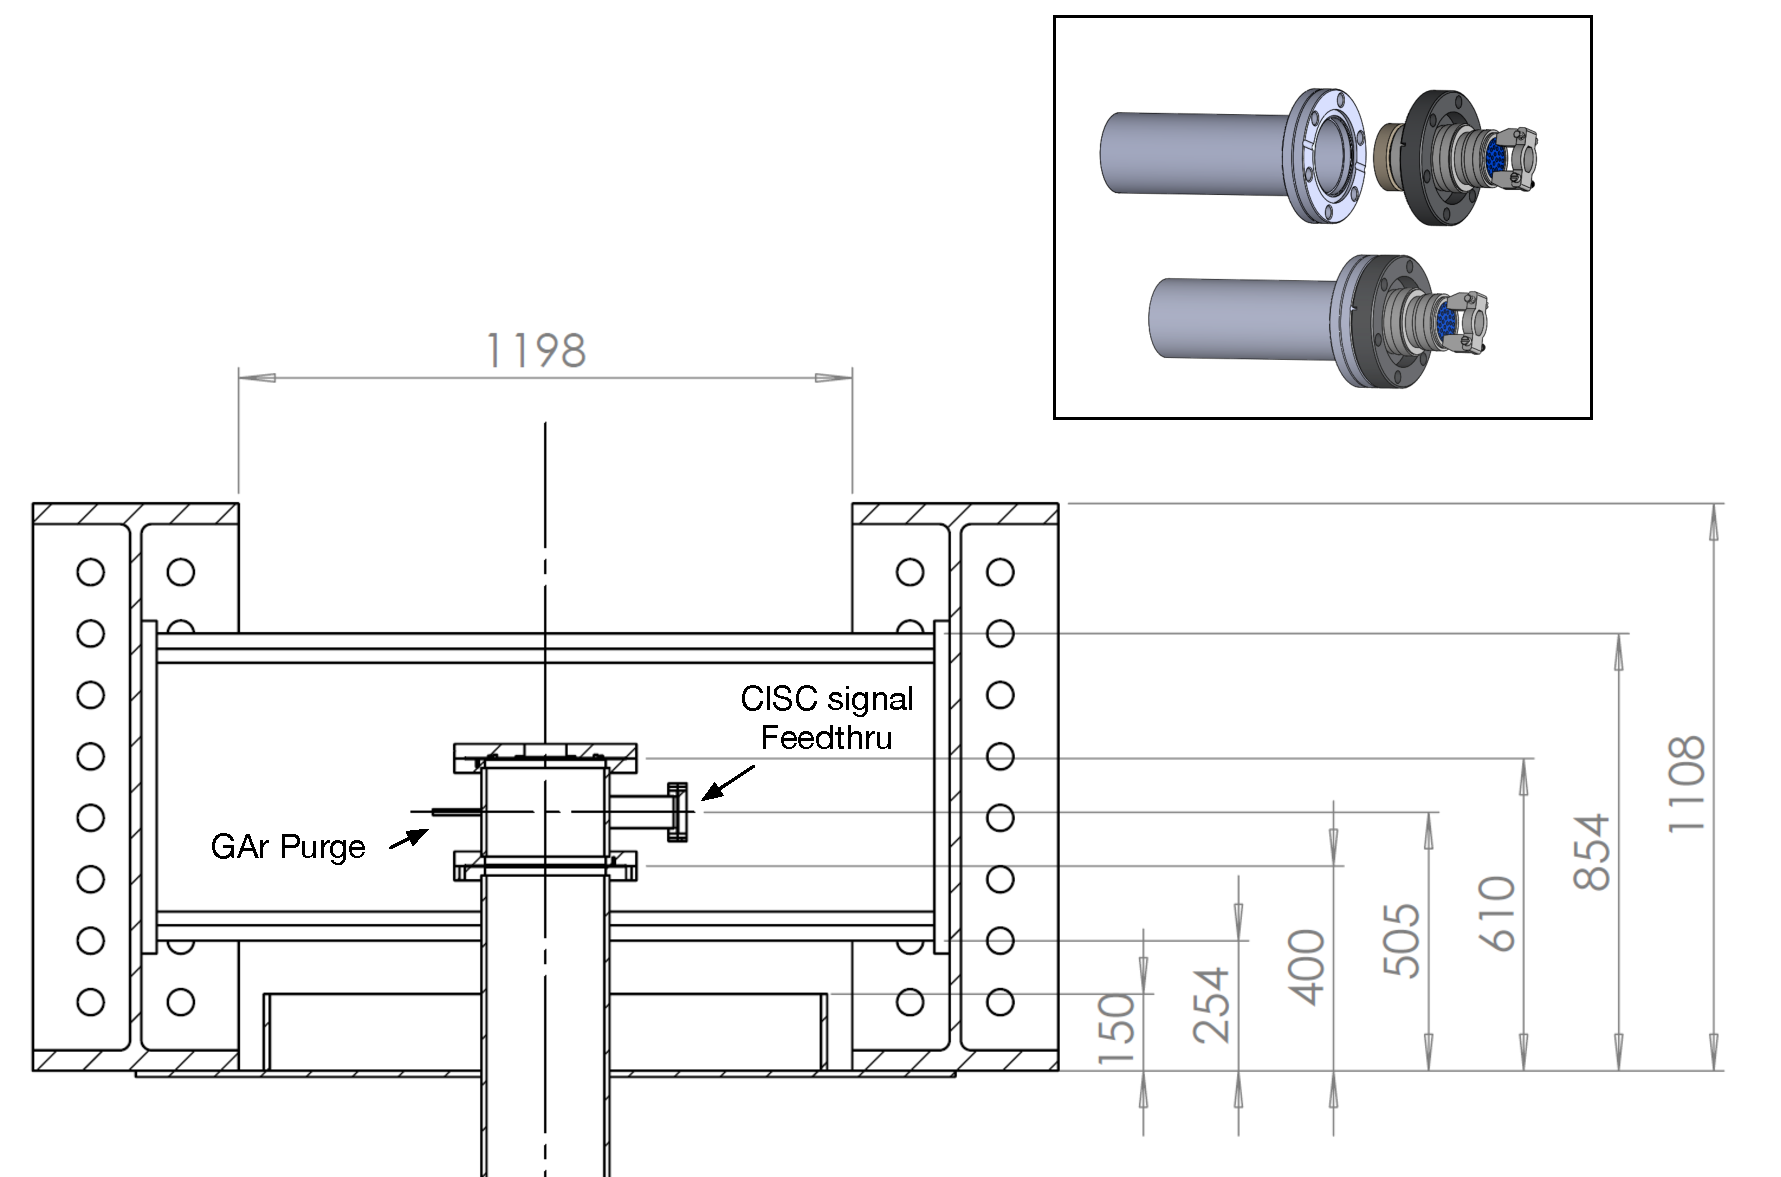
\includegraphics[width=0.95\textwidth]{CISC-feedthru.pdf}
\end{dunefigure}



%The first detector equipment to be installed are CISC thermometers,\fixme{SG: I think "CISC thermometers" is confusing since CISC has several types of thermometers. 

The first detector equipment to be installed are \dword{cisc} T-gradient thermometers, \fixme{SG: T-gradient correct? anne} an array of purity monitors, and cameras all at the east end of the cryostat. This equipment will be used to monitor the cool down, filling, and commissioning of the detector. Some equipment for the laser calibration system is also installed at this time, including some positioning diodes and possibly an optical mirror-based switching system.  The signals exit the cryostat using electrical feedthroughs distributed across the cryostat roof and integrated with the \dword{dss} support structure, as shown in Figure \ref{fig:CISC-feedthru}. Because all these components are small, they can be installed using a scissor lift with 12 \si{m} reach. At present, this is the tallest battery operated (thus cleanroom compatible) scissor lift rated for use in the USA that we have identified.



Cabling for the remaining static T-gradient monitors is also installed early before the start of \dword{tpc} installation.  The thermometer cables and mechanical supports are anchored to the cryostat using the bolts running along the cryostat's top and bottom edges and can be installed once the cryostat is clean. 
To avoid  damaging the small and fragile thermometers, they are not plugged into the small IDC-4 connectors until just before the corresponding \dword{apa} is moved into its final position. 
Cables and supports for the thermometers on the pipes below the detector and on the cryostat floor are installed immediately after installing the static T-gradient monitors on the walls.  Again the thermal sensors themselves are installed later, just before unfolding the bottom \dwords{gp}, to avoid damage.

Individual sensors on the top \dword{gp} must be integrated with the other \dwords{gp}. For each \dword{cpa} (with its corresponding four \dword{gp} modules), cable and sensor supports will be anchored to the \dword{gp} threaded rods. Once the \dword{cpa} is moved into its final position and its top \dwords{gp} are ready to be unfolded, sensors on these \dwords{gp} are installed.

 
Installing fixed cameras is, in principle, simple but involves a large number of interfaces. The enclosure for each camera has exterior threaded holes to facilitate mounting the camera on the cryostat wall, cryogenic internal piping, or \dword{dss}. Each enclosure is attached to a gas line to maintain appropriate underpressure in the fill gas, requiring an interface with cryogenic internal piping. Camera cables are run through cable trays to flanges on assigned instrumentation \fdth{}s. 


A summary of all the cryogenics instrumentation provided by the \dword{cisc} consortium is shown in Figure~\ref{fig:cisc_devices}. 

At this point the quartz optical fibers required for the \dword{pd} monitoring system are   run from the optical flange locations (still being finalized) to locations on the \dword{cpa} support beams of the \dword{dss}, to be connected later to the diffusers mounted on the \dword{cpa}s.


The residual gas analyzers that monitor for impurities in the \dword{gar} system must be installed before the piston purge and gas recirculation phases of cryostat commissioning.  However the actual time when they are installed depends on the schedule for outfitting the mezzanine and installing the  \dword{gar} purge piping. These  instruments are installed near the tubing switchyard to minimize tubing run length and for convenience when switching the sampling points and gas analyzers. 

\begin{dunefigure}[Distribution of various \dword{cisc} devices inside the cryostat.]{fig:cisc_devices}
  {Distribution of various %instrumentation 
  \dword{cisc} devices inside the cryostat}
  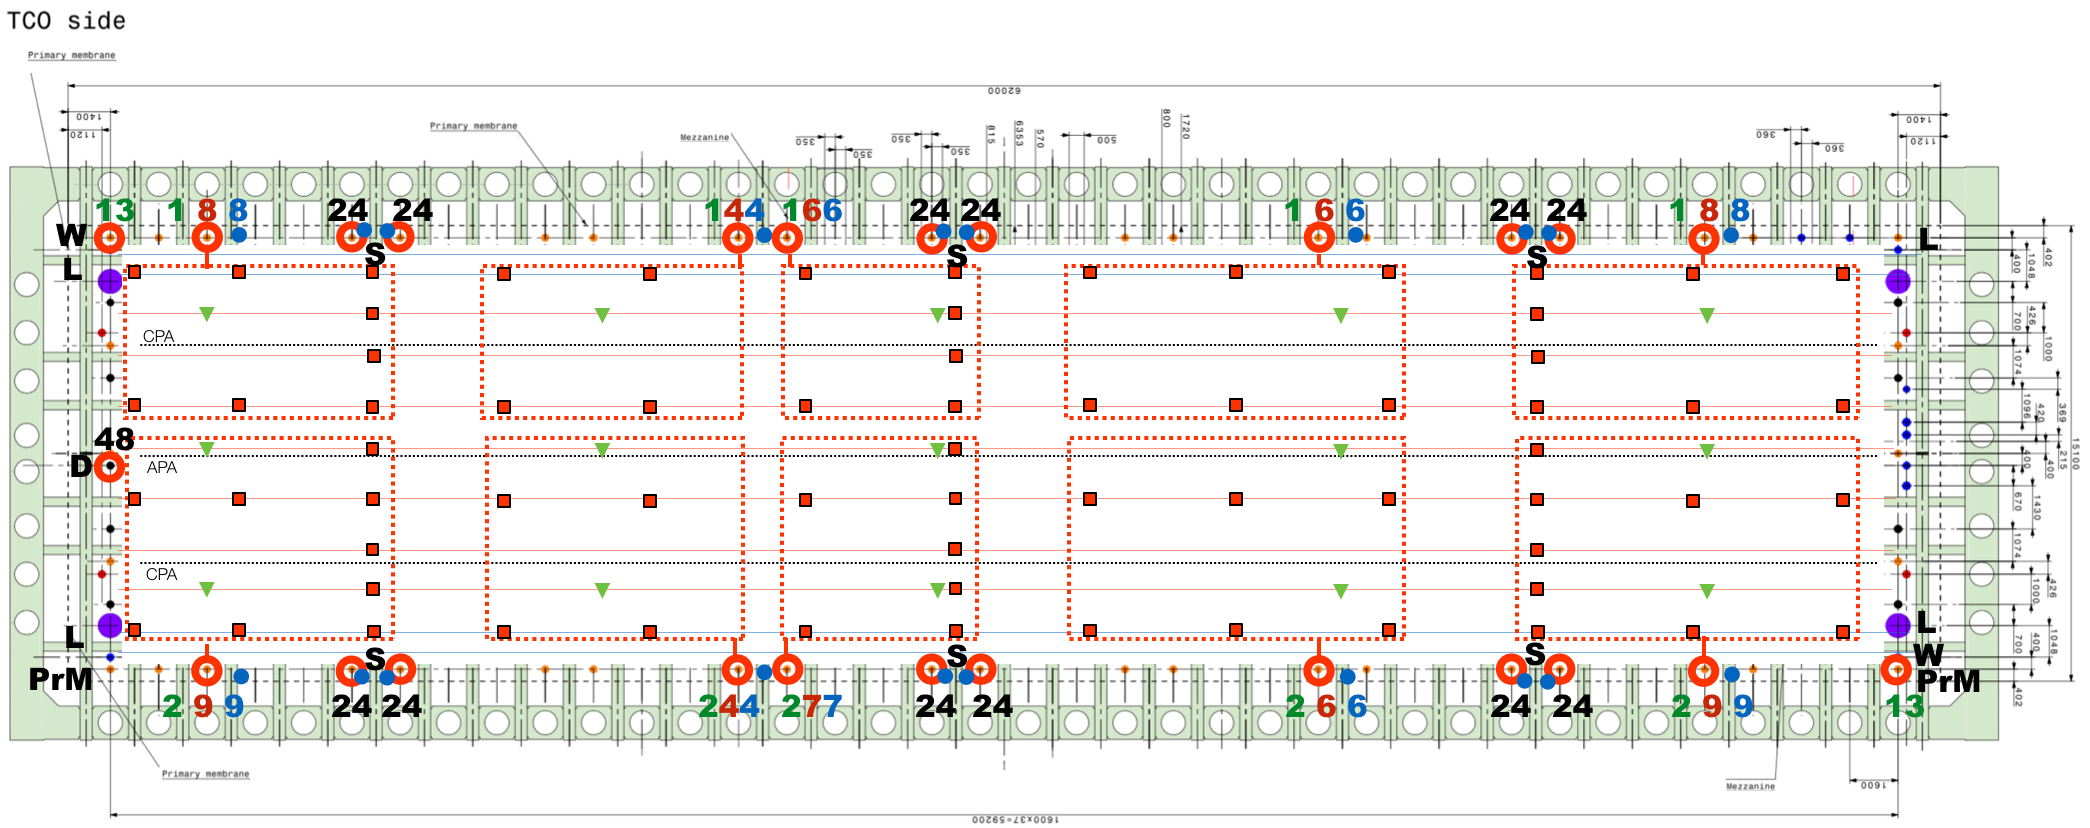
\includegraphics[width=0.98\textwidth]{cisc_distribution.png}
  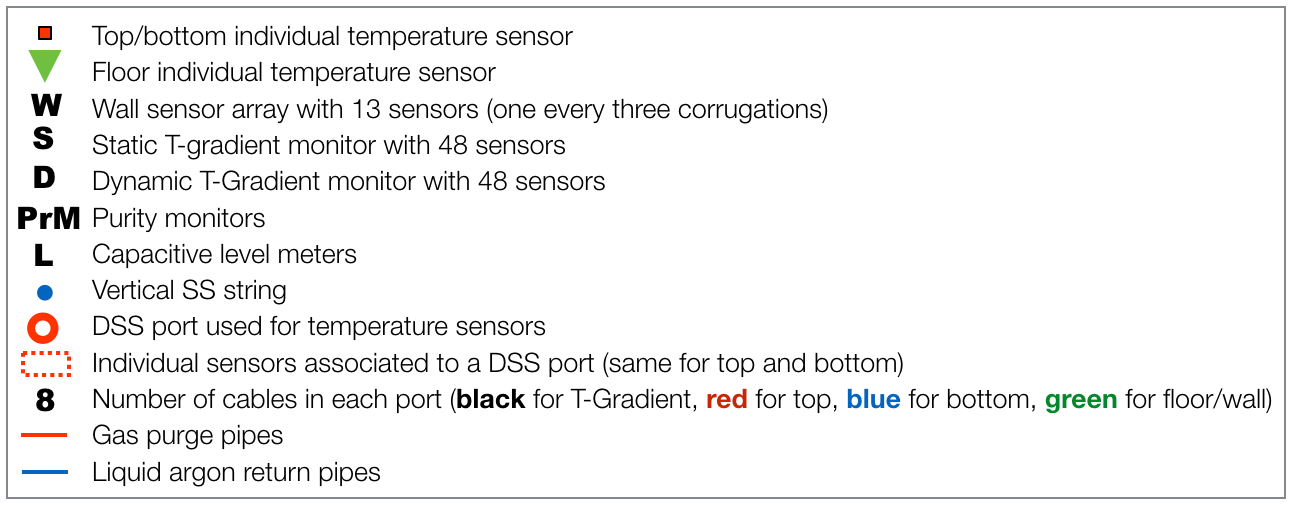
\includegraphics[width=0.85\textwidth]{cisc_distribution_legend.png}
\end{dunefigure}

% clear the figure buffer before starting the next section
\clearpage



Next the east \dword{fc} endwall is installed. The endwall panels are brought underground in custom crates. Each of the eight crates holds four endwall sub-panels. \fixme{is sub-panel a term in \dword{hv} chap? check} Eight sub-panels are needed to build one complete \SI{12}{m} tall panel.  First a custom hoist is installed on the end of the \dword{dss} beam for lifting and assembling the sub-panels in place as shown in Figure \ref{fig:endwall-hoist}. The endwall transport crates are then brought to the material airlock using a forklift where they are cleaned.  Once clean, the crates are moved into the cleanroom and placed next to the \dword{tco}. Then a hoist running on the rails through the \dword{tco} lifts the endwall sub-panels onto the transport cart, which is then hoisted into the cryostat. Figure~\ref{fig:endwall-cart} shows an endwall sub-panel being transferred over to the transport cart. The top endwall sub-panel is then attached to the installation hoist and lifted out of the cart. When the sub-panel is free of  the cart, it is re-positioned so the second sub-panel can be attached to the first, and the pair is then lifted. This process is repeated until the full 12 \si{m} endwall \dword{fc} panel is assembled and can be attached to the \dword{dss}. 
Figure \ref{fig:endwall-hoist} shows an endwall panel being lifted into position.
All the \dword{hv} connections inside the panel can now be tested. The process is then repeated for the remaining three endwall panels comprising the east endwall assembly. 

\fixme{check endwall vs panel vs sub-panel in pgraph above}
 
 \begin{dunefigure}[Endwall hoisting infrastructure]{fig:endwall-hoist}
  {Image showing the hoisting equipment used to lift the endwall into position. In this image, one of the endwalls is in place and a second is being positioned.}
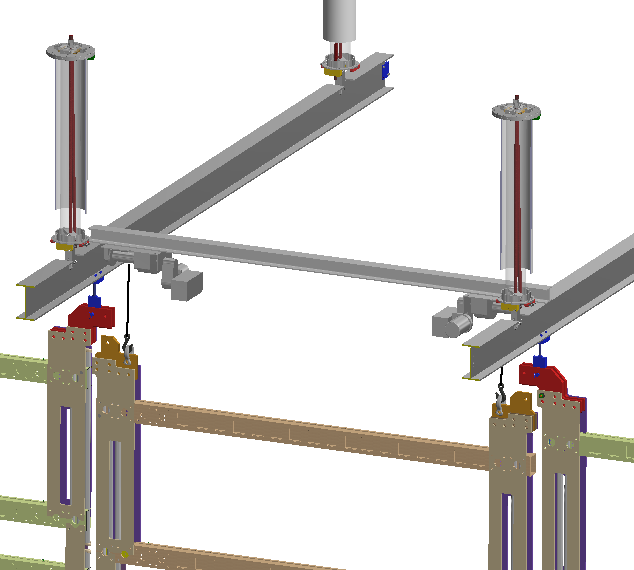
\includegraphics[width=.5\textwidth]{endwall-hoist}
\end{dunefigure}
 
\begin{dunefigure}[Installation of the first endwall]{fig:endwall-cart}
  {The endwalls are lifted out of the transport crates using the one of the hosts on the installation switchyard. Each panel is then placed on a custom cart that is then lifted into the cleanroom.}
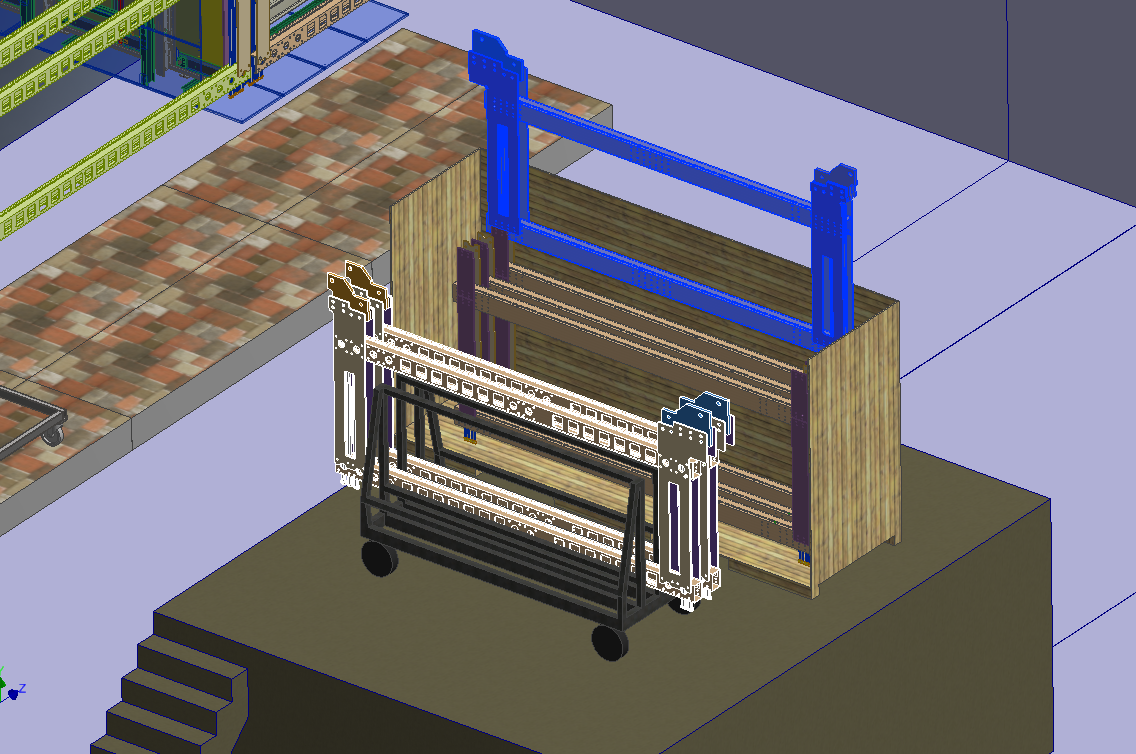
\includegraphics[width=.5\textwidth]{endwall-cart}
\end{dunefigure}




The installation of an \dword{apa} and  \dword{cpa} with top and bottom \dword{fc} modules is the most labor-intensive part of the detector installation. Figure \ref{fig:install-single-row} represents one of the 25 rows of \dword{tpc}.  \dword{dune} aims to perform work in parallel to the extent possible and finish installing one row every week. 
This requires that several separate teams work in the cleanroom, inside the cryostat, and on the cryostat roof simultaneously --  positioning the equipment, integrating \dword{pd} into the \dword{apa}, mounting the \dword{ce} \dword{femb} on the \dword{apa} connecting the cables, cold testing \dword{apa}, installing \dword{apa} in the cryostat, assembly and installing \dword{cpa}/\dword{fc} and deploying the \dwords{fc}.
Figure \ref{fig:Single-APA-Schedule} shows the labor breakdown and activities in the airlock,  cleanroom, and cryostat for the \dword{apa} installation. These labor estimates will be refined during time and motion studies at Ash River. As this installation process is  complicated it will be described in steps: first the \dword{apa} assembly work in the cleanroom is described followed by the \dword{cpa} assembly and then finally the installation process inside the cryostat.

While the \dword{apa}s \dword{cpa} and \dword{fc} are installed, the area outside the cleanroom in the north cavern is available for storage; this area has sufficient capacity to store one full month's worth of equipment. Equipment will be brought into the cleanroom's materials airlock through a roll-up or curtain door in the west wall using either an electric forklift or electric pallet jacks.

\begin{dunefigure}[Single row of APA and CPA]{fig:install-single-row}
{One row of the \dword{apa} and \dword{cpa} with associated field cages is shown. In this  image, the \dwords{fc} are deployed in the final orientation. The equipment in the figure represents $1/25$ of the total TPC.}
 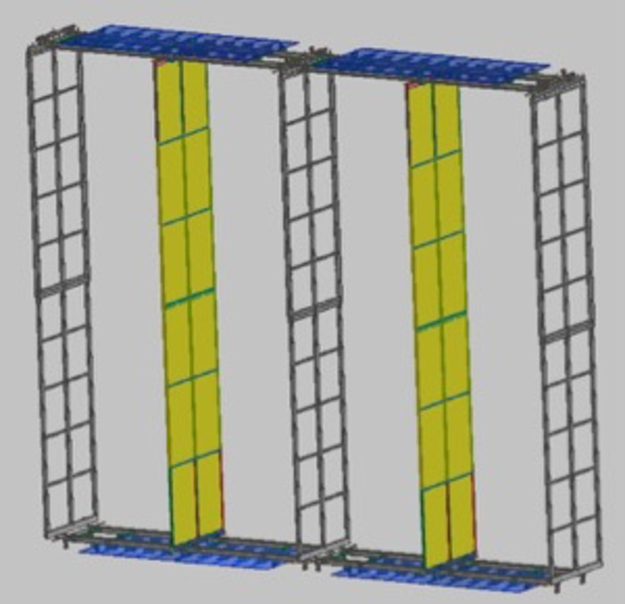
\includegraphics[width=0.3\textwidth]{install-single-row}
\end{dunefigure}

\begin{dunefigure}[Typical APA installation schedule]
{fig:Single-APA-Schedule}
{Typical \dword{apa} schedule for \dword{spmod}}
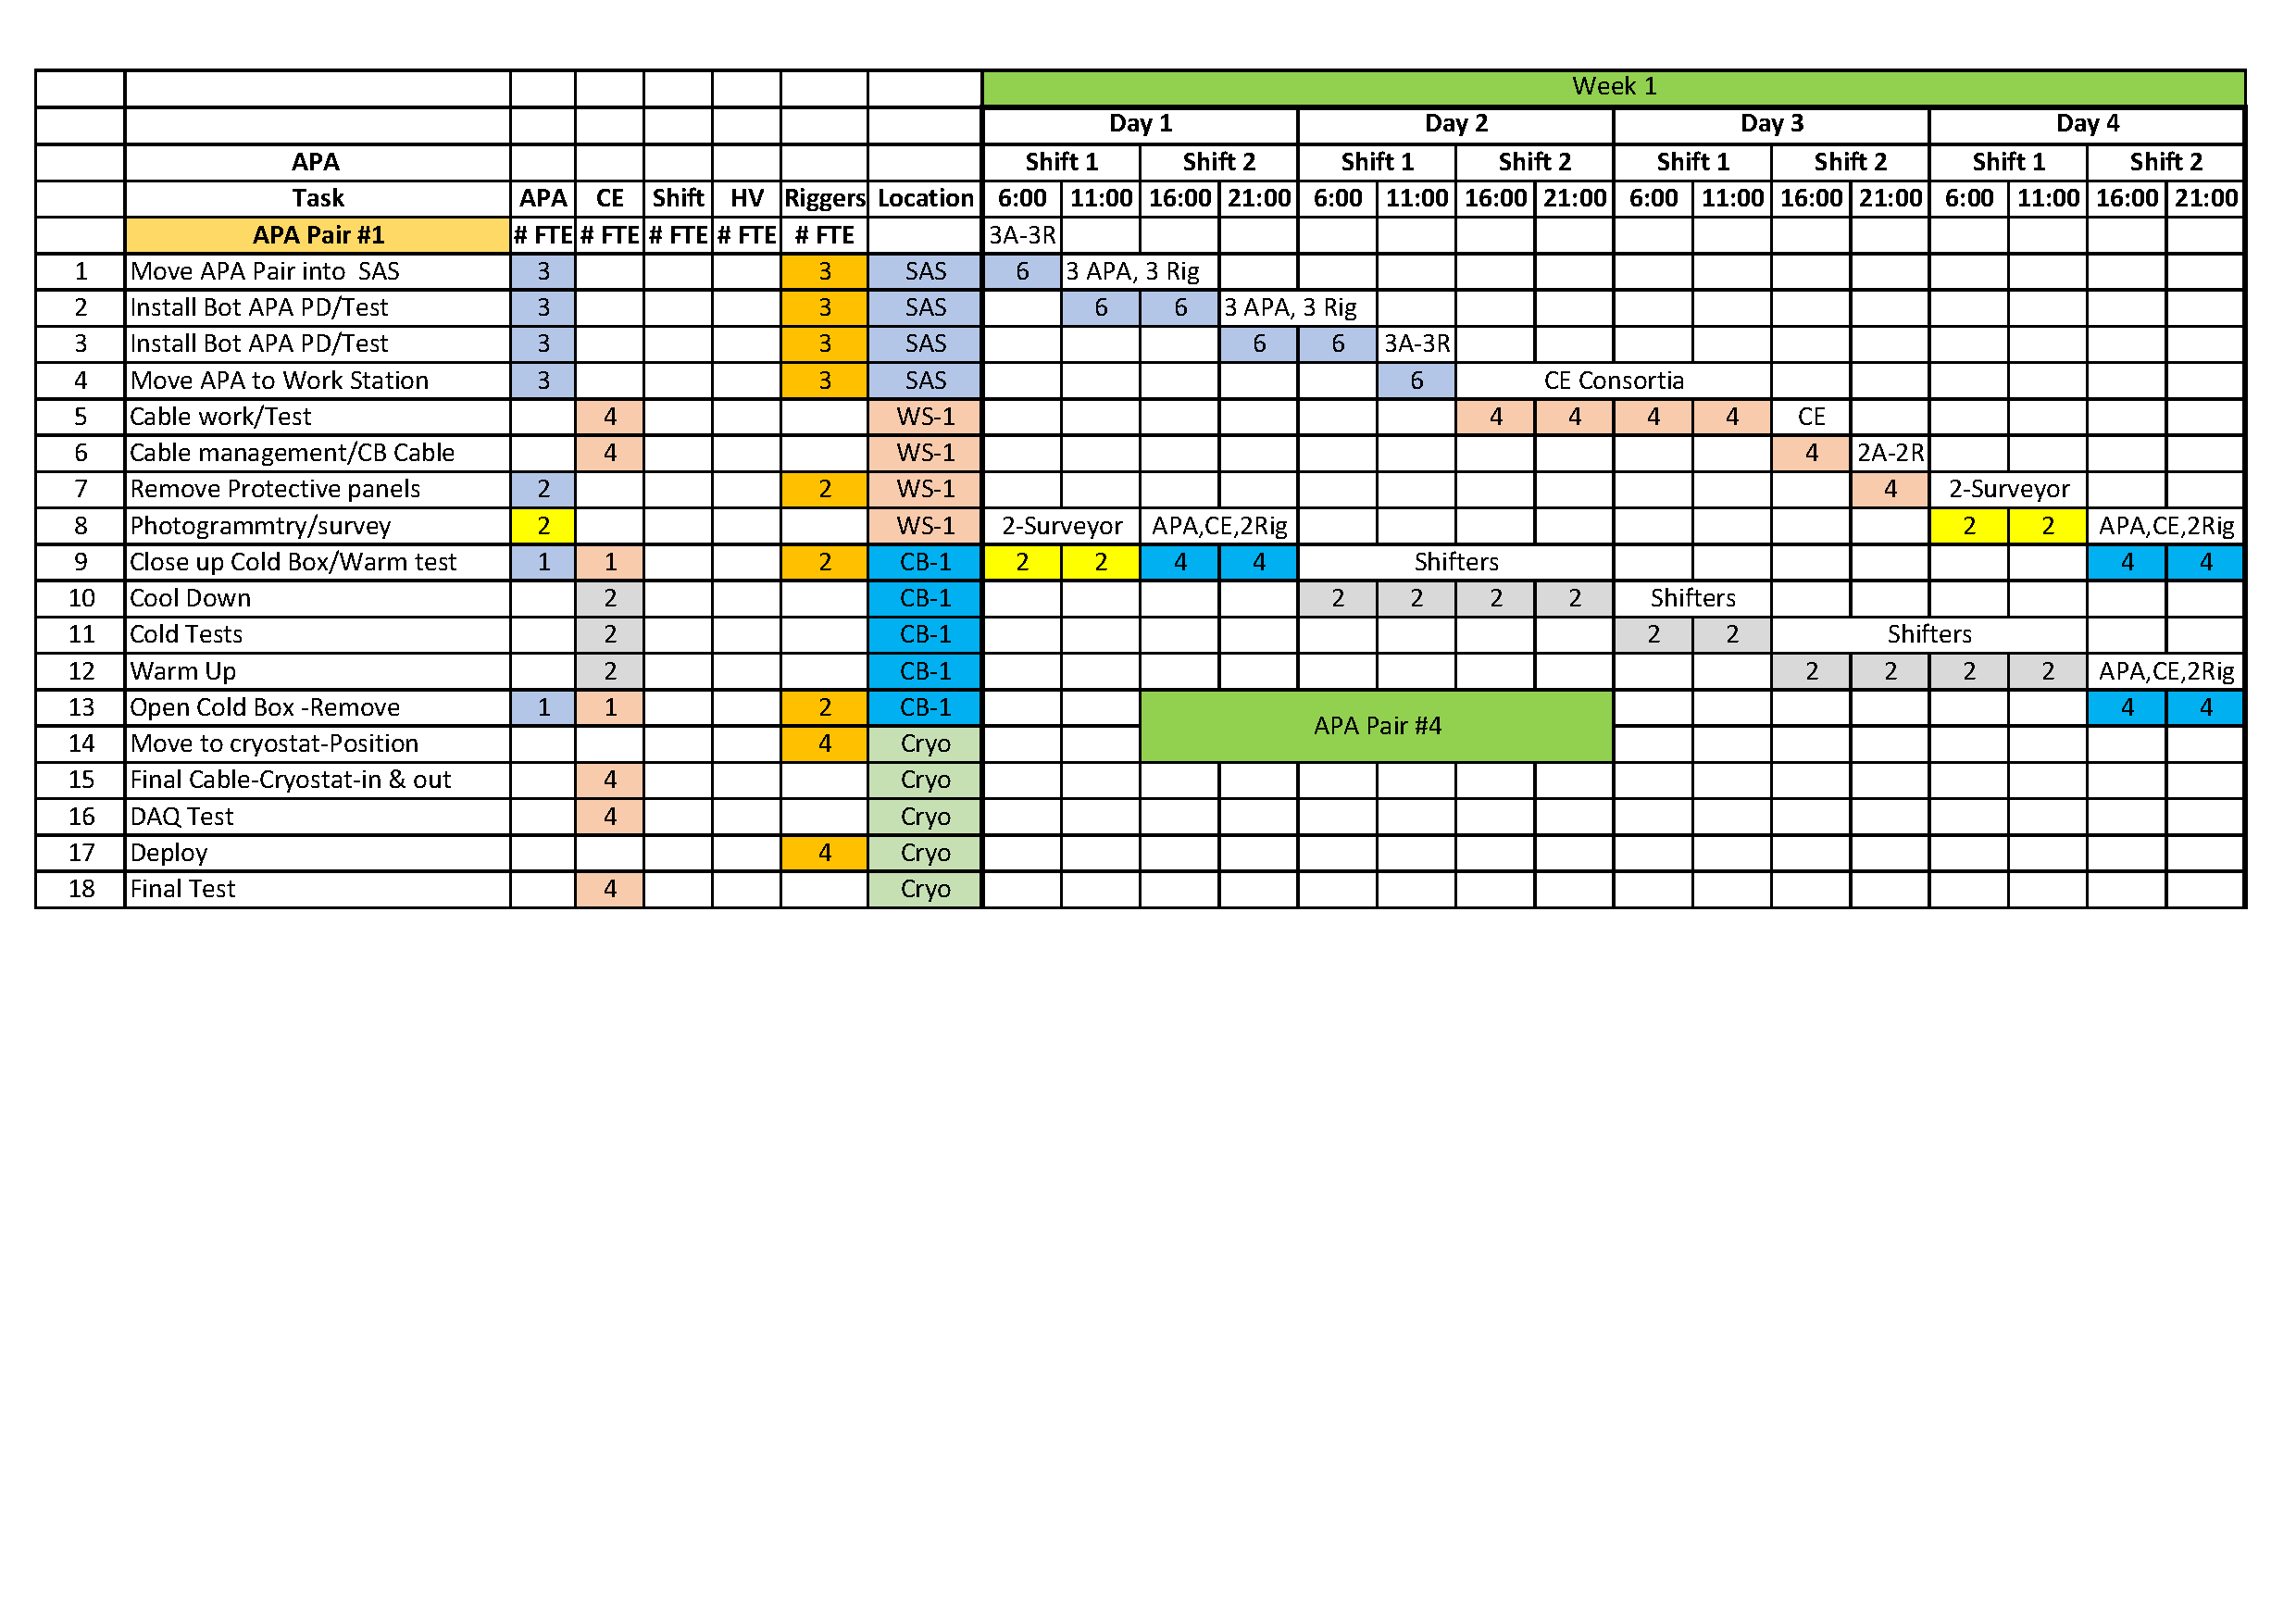
\includegraphics[width=0.95\textwidth]{Single-APA-Schedule.pdf}
\end{dunefigure}


  
An \dword{apa} transport crate which holds two \dword{apa}s  is first rotated to the vertical orientation and bolted to a custom weighted skid used for moving the crate in the cleanroom. 
Battery powered pallet jacks are used to move the crate into the materials airlock where the outer covers are removed and the outer frame cleaned. 
After the air purity has recovered the transport box can be bought into the cleanroom proper.
The \dword{apa} are first moved to the \dword{pd} integration area where the photon detectors are inserted into the sides of the \dword{apa}. 
The \dword{apa} transport boxes and \dword{apa} protective covers are designed to keep the slots in the sides for the photon detectors clear. 
The \dword{apa} transport box is places between two fixed scissor lifts. The transport box is situated so that two person teams in the lifts and easily hold a \dword{pd} module on the side of the lift. 
The lift is raised to align the paddle with one of the 5 slots in the side of the \dword{apa}. The paddle can then be slid into the side of the \dword{apa}. 
The guides inside the \dword{apa} frame ensure that the electrical connectors in the middle of the \dword{apa} mate easily. 
The \dword{pd} are locked in position with two captured screws. 
After each \dword{pd} is installed it can be tested electrically by accessing the connectors at the top using a scissor lift. 
Once the 10 \dword{pd} paddles are installed on first \dword{apa} the transport crate is shifted slightly and the photon detectors can be inserted into the second \dword{apa} and tested. It may be required to pull the \dword{apa} transport crate out from between the lifts to install the lowers \dword{pd} modules.

\begin{dunefigure}[Photon detector and anode plane assembly integration]
{fig:install-pd-integrate}
{Area where the photon detectors are integrated into the \dword{apa} modules. Floor mounted scissor lifts are used to access the sides of the \dword{apa}.}
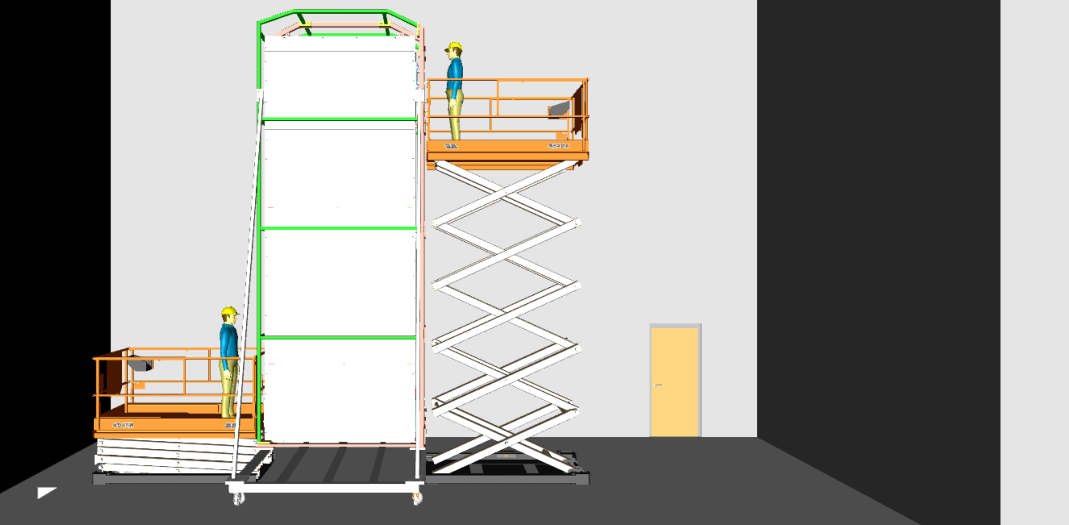
\includegraphics[width=0.75\textwidth]{graphics/install-pd-integrate.pdf}
\end{dunefigure}


\begin{dunefigure}[Initial APA testing and doublet assembly]
{fig:install-apa-prep}
{Initial \dword{apa} testing and assembly into doublets.}
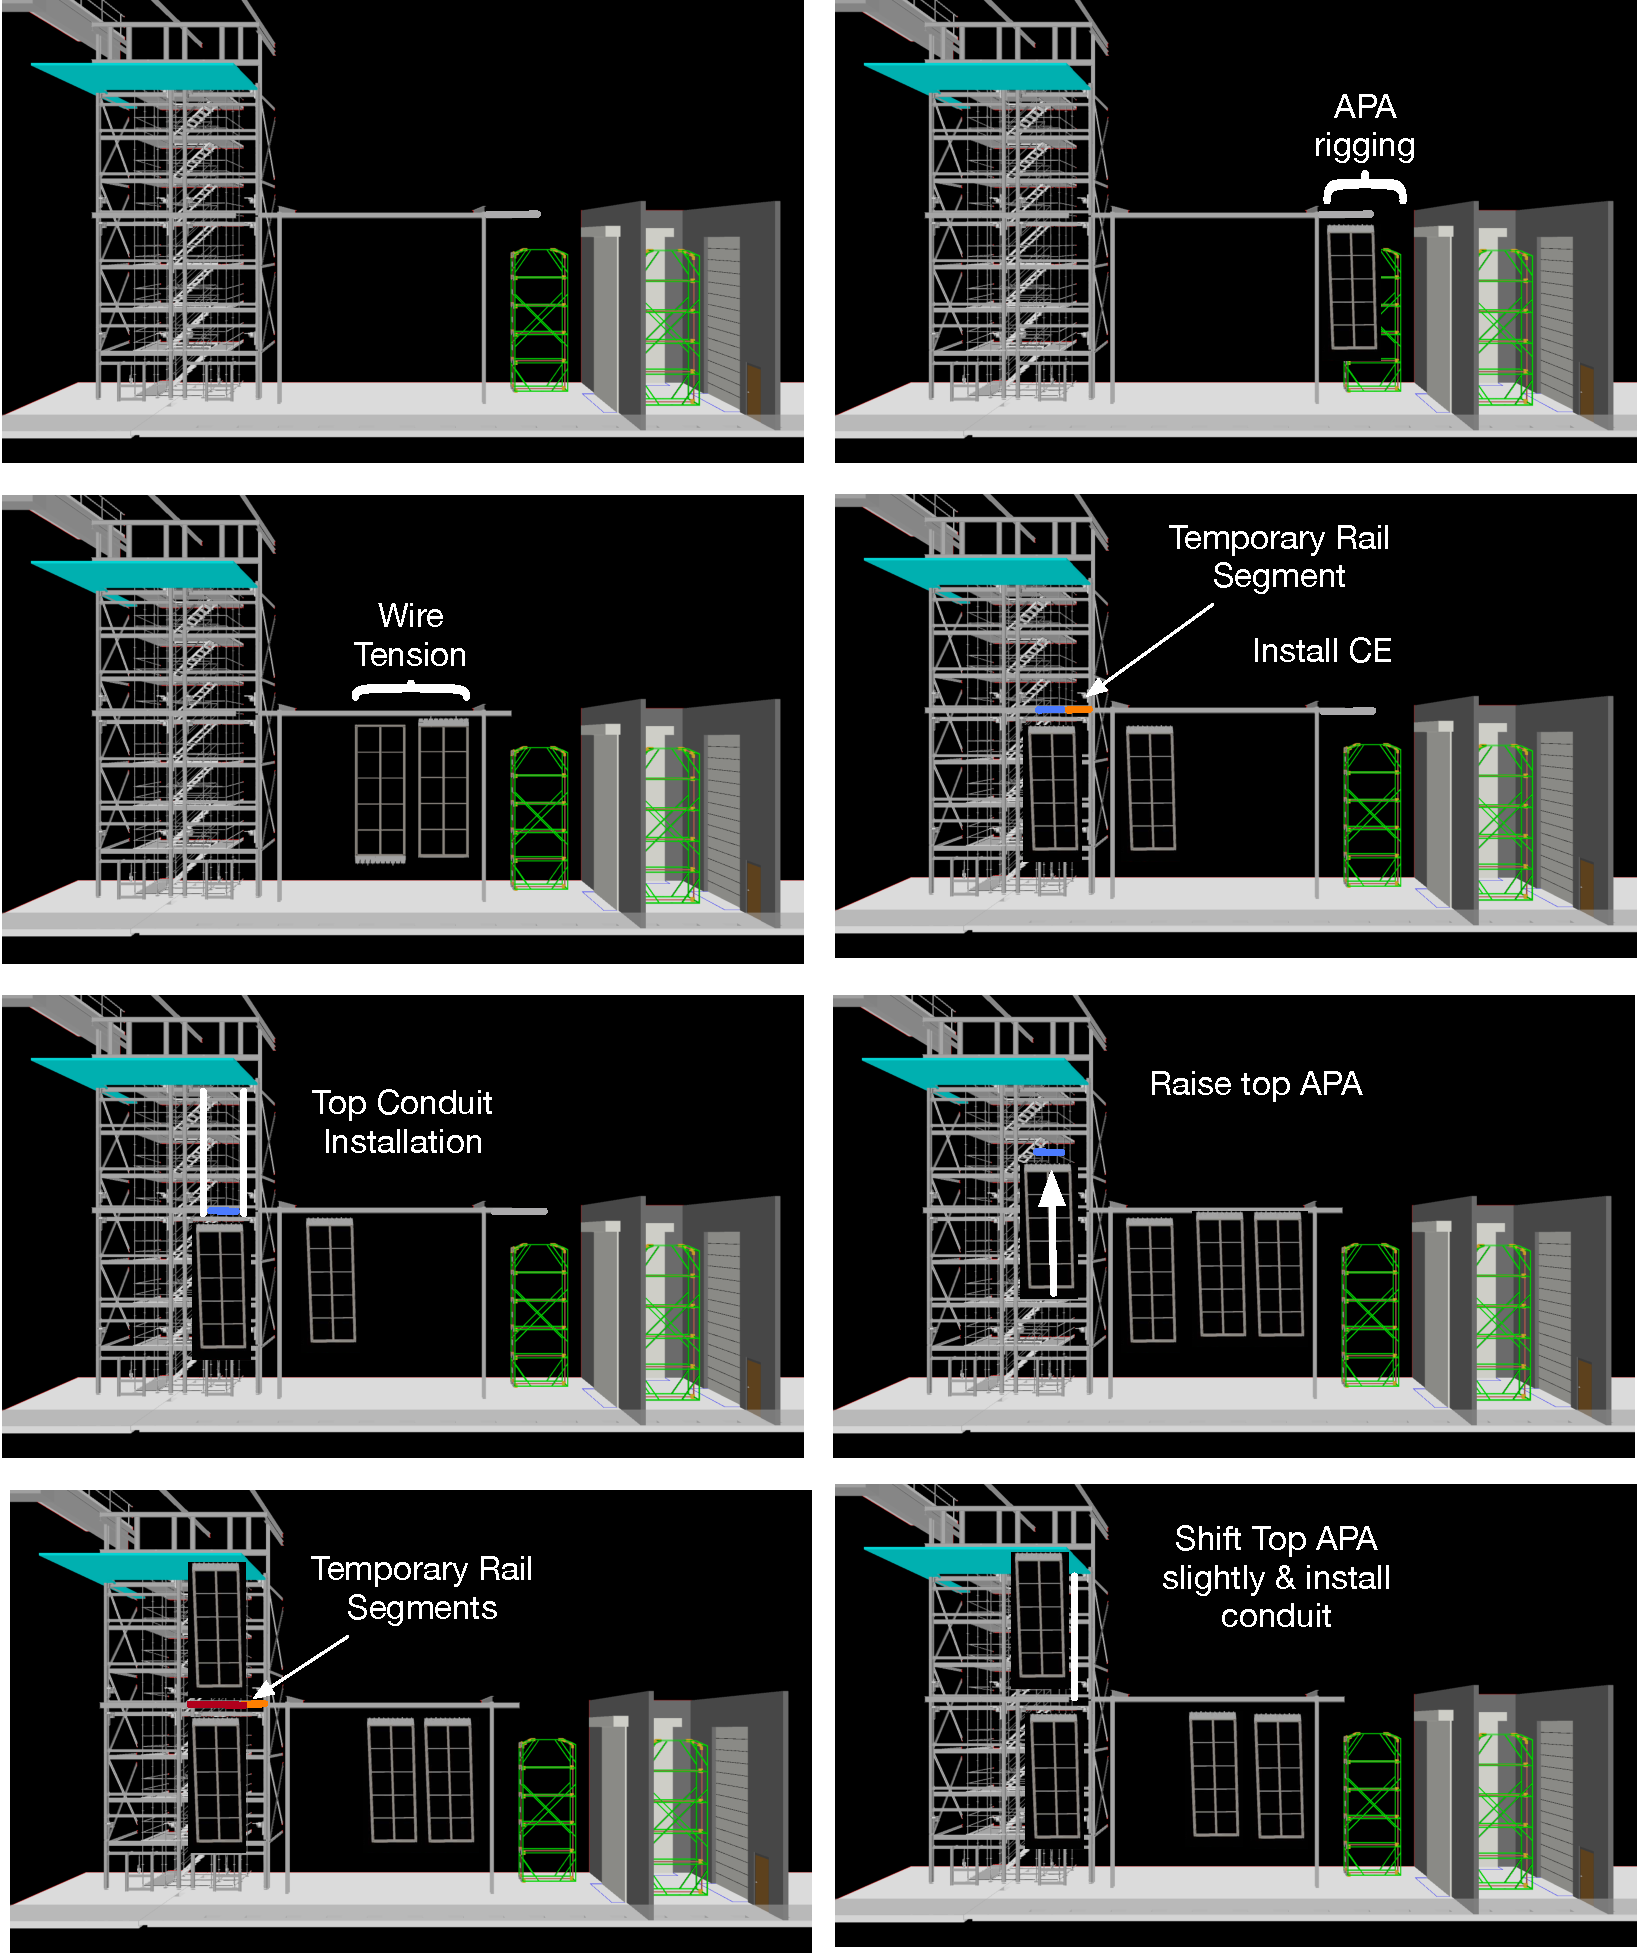
\includegraphics[width=0.95\textwidth]{install-apa-prep}
\end{dunefigure}

After the \dword{pd} integration and testing is complete the transport box with the two \dword{apa}s is moved to the start of one of four assembly lines. 
The initial time and motion studies indicate that three lines are sufficient to keep up with the cold testing and installation in the cryostat so one line is considered spare or for any needed repair. 
The side view of one assembly line is shown in Figure \ref{fig:install-apa-prep} and the initial assembly steps are illustrated. 
First a top \dword{apa} is removed from the transport box and mounted to trolleys on the assembly line rails. 
The \dword{apa} is shifted over to the top \dword{apa} tension measuring station and the protective covers are removed and a visual inspection performed. 
The bottom \dword{apa} then also needs to be mounted to the rail. 
However the bottom of the \dword{apa} cannot support the load of the \dword{apa}. 
Heavy duty rods are inserted into the sides of the \dword{apa} and bolted to the side tubes using the bolts designed for the linkage connecting the \dword{apa} pair. 
The \dword{apa} can then be hoisted out of the transport box and connected to the rail. 
Either the trolleys can be mounted directly to the rods or or a crossbar can be used between the support rods to hold the trolleys.
The lower \dword{apa} can then also be shifted to its tension measuring location and its protective covers are removed. 
Wire tension data is collected according to the \dword{qa} plan similar to \dword{protodune}. 
When the tension measurements are complete the protective covers are re-installed to protect the wires during the subsequent assembly steps. 
The top \dword{apa} is then shifted over to the first station on the \dword{apa} assembly tower. The rail lower rail across the tower is constructed in three removable pieces; the center section can either be fixed or connected to a hoist and lifted. Once the top \dword{apa} is attached to the center rail section the two outer sections can be removed and the cable conduits installed. 
The assembly tower area of the cleanroom has a roof height of \SI{17}{m} allowing the \SI{6}{m}conduit to be installed in the SI{6}{m} tall \dword{apa} easily. 
Once the conduit is in place the I-beam segment supporting the \dword{apa} is attached to a hoist and lifted to the upper rails and attached. 
Locking pins in the \dword{apa} assembly fixture then hold the top \dword{apa} rigidly in location. 
It will be investigated if the assembly fixture can be modified so the guides can travel with the \dword{apa} when it is lifted thus providing stability against rotation. 
The lower \dword{apa} is then moved to the position where it can be connected to the  assembly fixtures. 
Now the  lower \dword{apa} is supported from the bottom, and guides connected to the sides of the \dword{apa} provide mechanical stability while allowing the \dword{apa} to be lifted using jacks integrated into the lower support. 
At this time the lower \dword{apa} is held by the assembly fixture and the I-beam a the top can be removed along with the transport rods in the side tubes. 
The conduit is installed by freeing the top \dword{apa} and shifting it slightly to allow the conduit to be inserted from the top through the foot tube. 
The \dword{apa} is then moved back in position and again locked to the \dword{apa} assembly fixture.
The lower \dword{apa} \dword{pd} paddles are then tested to ensure everything is working.
At this point, the upper \dword{apa} is supported by the trolleys that move the \dword{apa}s along the upper transport rails, and it is stabilized using the \dword{apa} assembly frame. There is a 300-500 \si{mm} gap between the upper and lower \dword{apa}, so now the photon cables between upper and lower \dword{apa} can be connected, and the connection from the top connectors to the SiPMs can be checked. 
To mechanically connect the two \dword{apa} modules, a metal linkage with electrical insulators is inserted into the upper \dword{apa} and bolted into place. Then the lower \dword{apa} is raised until the linkage can be bolted to the lower \dword{apa}.  
The \dword{apa} pair can then be released from the assembly tower supports and jacks; it is now supported from the top, where the upper \dword{apa} connects to the transport rail system. The \dword{ce} boxes can then be installed at the top and bottom of the \dword{apa} doublet. The \dword{apa}s can then be shifted over to the second station on the assembly tower where the cabling is done.




\begin{dunefigure}[APA cabling and cold test]{fig:apa-assembly-v4}
  { Left to right: cables being inserted in the \dword{apa} doublet; \dword{apa} doublet moving on the cleanroom transport rails; and the \dword{apa}s being inserted into the coldbox.}
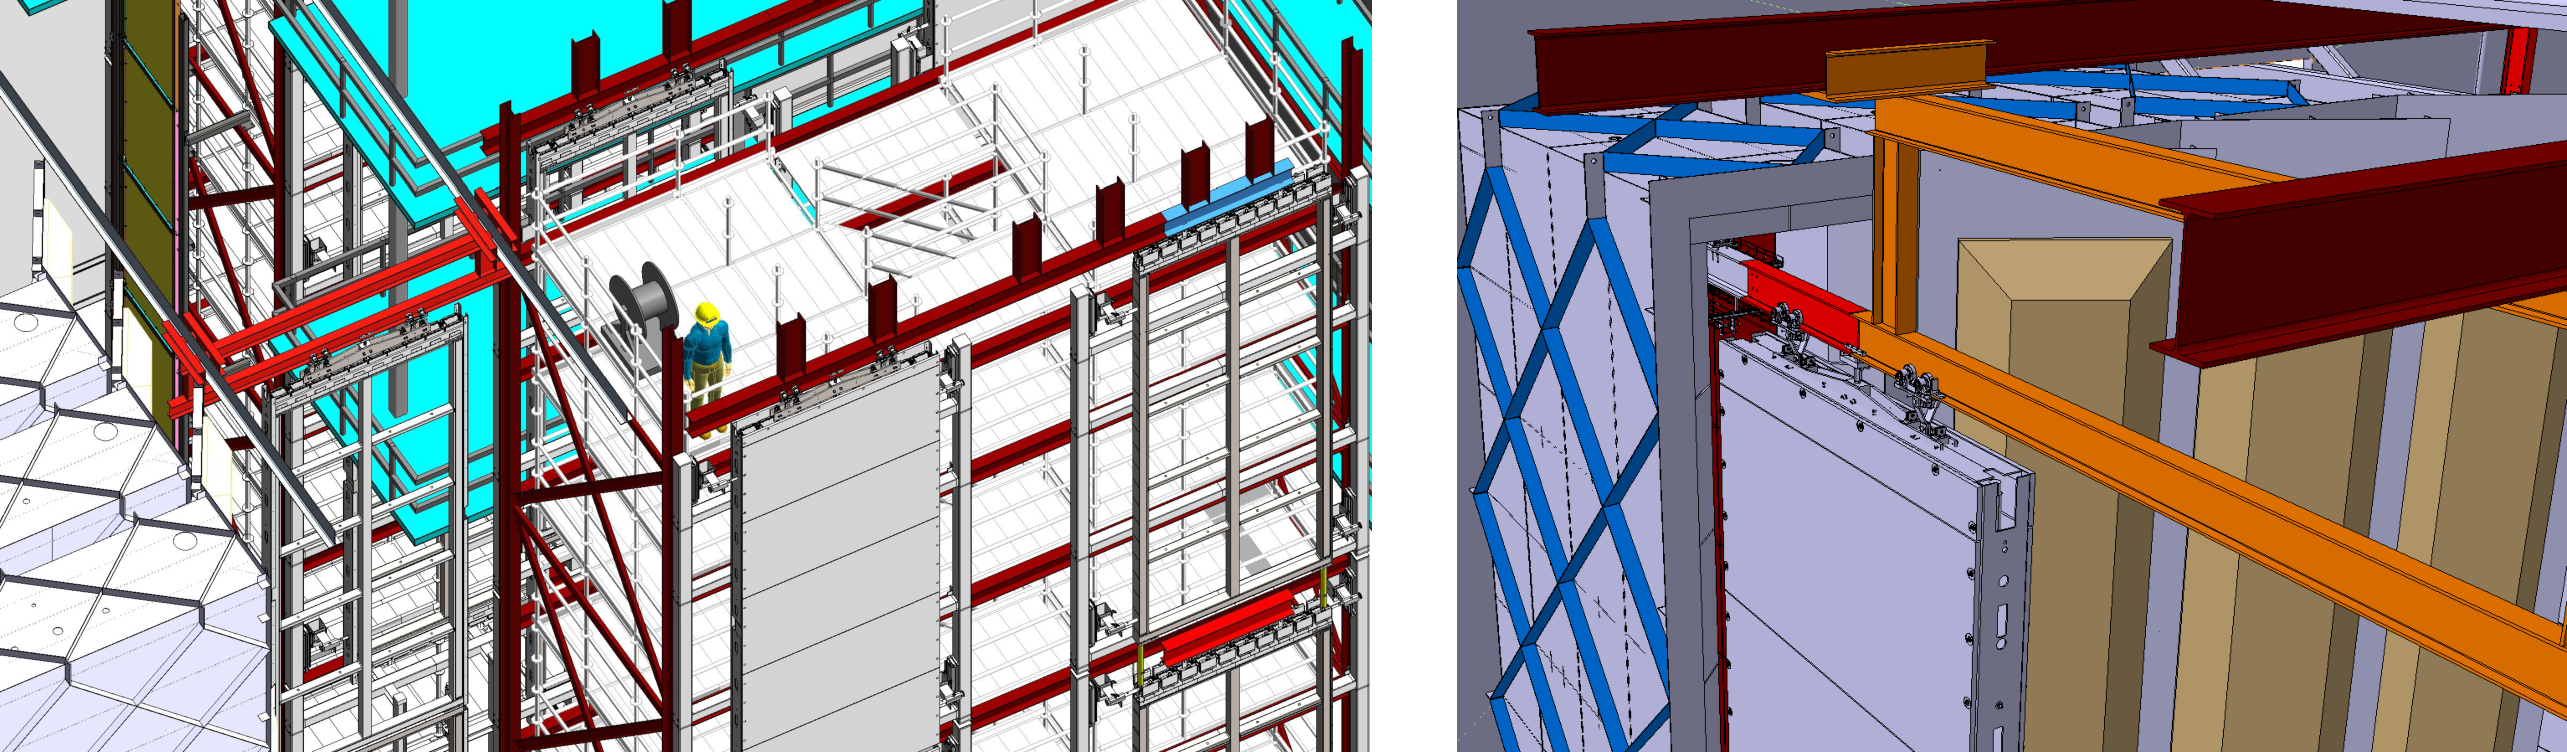
\includegraphics[width=.9\textwidth]{apa-assembly-v4}

\end{dunefigure}

The next assembly step is to install and test the electronics cabling.  The lower left image in Figure \ref{fig:apa-assembly-v4} shows the \dword{apa} cabling area on the \dword{apa} assembly tower. 
The electronics cables are delivered to the cleanroom on reels pre-bundled and tested. Images of the cable assembly are in the \dword{ce} section Figure XX.
\fixme{need reference from the CE section} 
The switchyard crane lifts the lower \dword{apa} cable reels to the top of the assembly tower, and a cable is then spooled over to a motorized deployment spool. 
The cable guide is then attached and fed through a guide sheave and into the conduit on the side of the \dword{apa}. The cable bundle is carefully fed through the conduit and anchored in place using a cryogenic compatible cable grip. The cable is connected to the electronics at the bottom and is laid into the cable trays on top. This process is repeated for the second lower \dword{apa} cable bundle. 
Finally, the upper \dword{ce} and \dword{pd} cables can be installed and prepared for transport.

At this time, the functionality of all the electronics is checked. 
After the \dword{apa} electrical test, the \dword{apa} pair is moved onto the switchyard where the protective covers are removed and the assembly surveyed using photogrammetry. 
The \dword{apa} pair is then transported to a coldbox where it undergoes a thermal cycle and complete systems test. 
The right image in Figure \ref{fig:apa-assembly-v4} shows the \dword{apa} being inserted into the coldbox. The coldbox is also a Faraday cage, so noise levels can be measured and the photon system checked for photon sensitivity. 
After the cold test is complete, an \dword{apa} will either move back to the cabling station if any repair is needed, or it will be moved into the cryostat for installation. 


\begin{dunefigure}[CPA assembly steps]{fig:install-cpa-assembly}
  {The \dword{cpa} assembly steps are shown. Top row from left:  \dwords{cpa} are delivered to the CPA assembly fixture in the cleanroom; the 3 \si{m} sub-panels are lifted onto the frame and connected. Bottom row from left: After the CPA panel is complete, it is moved into the room and the field cage modules are attached. The CPA is then moved into the cryostat.}
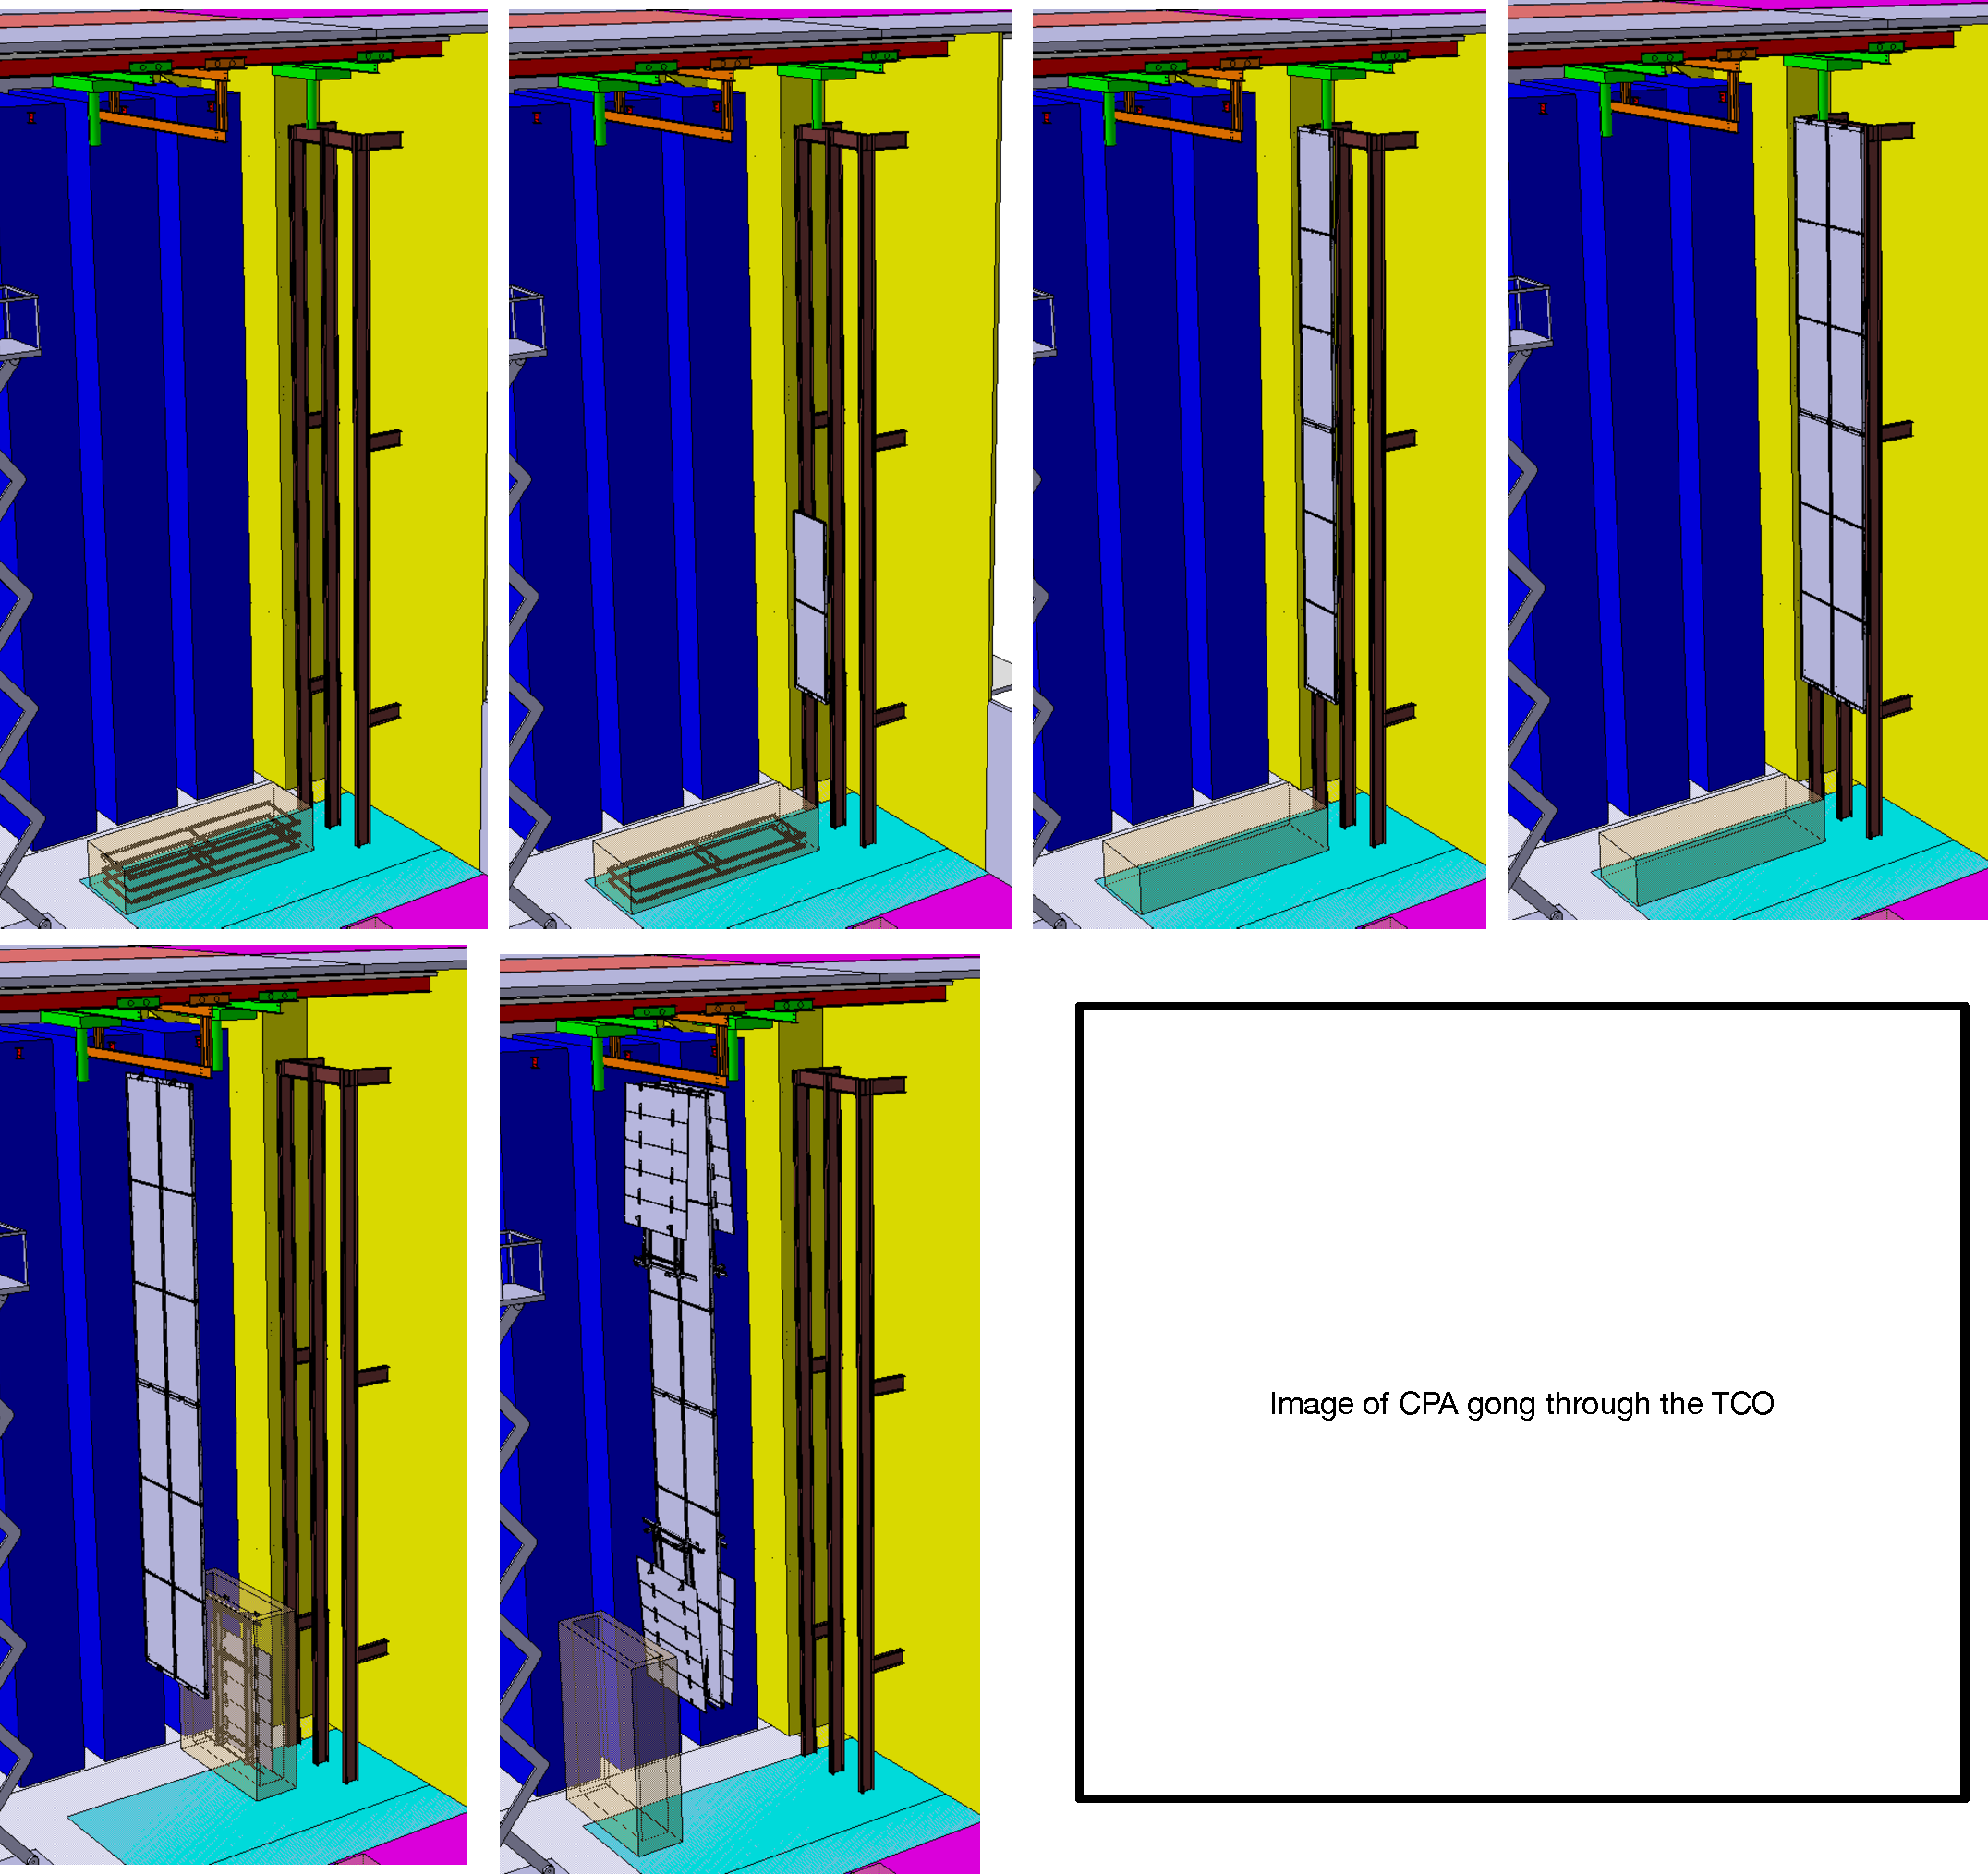
\includegraphics[width=.9\textwidth]{install-cpa-assemble}
\end{dunefigure}

The CPA and top \dword{fc} modules are assembled in parallel to the \dword{apa} assembly. Figure \ref{fig:install-cpa-assembly} shows the  assembly sequence. The sub-panels for the cathode plane are delivered to the airlock in crates that hold 4 \si{m} long 1.15 \si{m} wide segments. After cleaning, the crates are brought into the cleanroom and opened. The panels inside are bagged to provide additional dust protection. The sub-panels are lifted out of the crate and placed on the assembly frame using the cleanroom switchyard hoist. First one of the 1.15 \si{m} 4 
\si{m} tall sections is assembled, followed by the second and third ones. The 1.15 \si{m} wide section is then lifted, connected to the installation switchyard, and moved to the \dword{tco} beam. The second 12 \si{m} tall section is then assembled like the first. The two 1.15m wide panels are then connected to make the 2.3 \si{m} wide unit.  A complete set of \dword{qc} measurements are taken of all electrical connections between panels.  The cathode assembly  is then moved to a location in the switchyard where the diffuser fibers and top field cage modules can be installed.
 The top \dword{fc} modules are then attached. In Figure \ref{fig:install-cpa-assembly}, the completed assembly is shown with the lower \dword{fc} modules also attached. This is an option, but present planning is to install the lower \dword{fc} modules  inside the cryostat. Finally, the \dword{cpa}-\dword{fc} assembly is moved into the cryostat.


\dword{pd} monitoring system optical diffusers and short optical fibers must be connecetd to the \dword{cpa} panels before the panels are installed in the cryostat.  Discussions are underway about the optimal site for this installation:  at the \dword{cpa} assembly facility before shipping to the site, or as part of the assembly of \dword{cpa} stacks in the underground cleanroom.  Whichever solution is adopted, quartz optical fibers must be routed from the diffuser to the top of the \dword{cpa} assembly to be connected later to the pre-installed fibers in the cryostat; this connection will occur upon final positioning of the \dword{cpa}.  

Work inside the cryostat will proceed in parallel with the work in the outer cleanroom. 
The large detector components like \dword{apa} pairs and \dword{cpa} modules will enter the cryostat using the \dword{tco} rails that connect to the \dword{dss} switchyard.
Inside the cryostat, the modules will be pushed onto one of the switchyard shuttle beams shown in  Figure \ref{fig:shuttle}. 
The \dword{dss} shuttle beam is then moved to the appropriate row of the \dword{dss}, and then the module is pushed down the length of the cryostat into position. The position of the \dword{dss} beams are well defined and accurately surveyed so the \dword{apa} and \dword{cpa} modules can be accurately located by precisely positioning them along the \dword{dss} beams. A small correction in the height of the modules may be needed to accommodate deflections in the \dword{dss} due to load. Figure \ref{fig:install-ce-cables} shows the typical situation during the \dword{apa} installation and \dword{ce} cabling. 

\begin{dunefigure}[Cold Electronics cabling inside the cryostat]{fig:install-ce-cables}
  {The installation of the APA and cabling of the cold electronics is described. The left panel shows the APA installation process. One row of APA and \dword{hv} equipment is installed, and a second APA is ready for electrical cabling. The top right image shows the cable trays that will hold the CE cables; one worker is in the scissor lift. The left bottom image shows the work space with the geometry of the APA, the cryostat roof, and the cable feedthrough.}
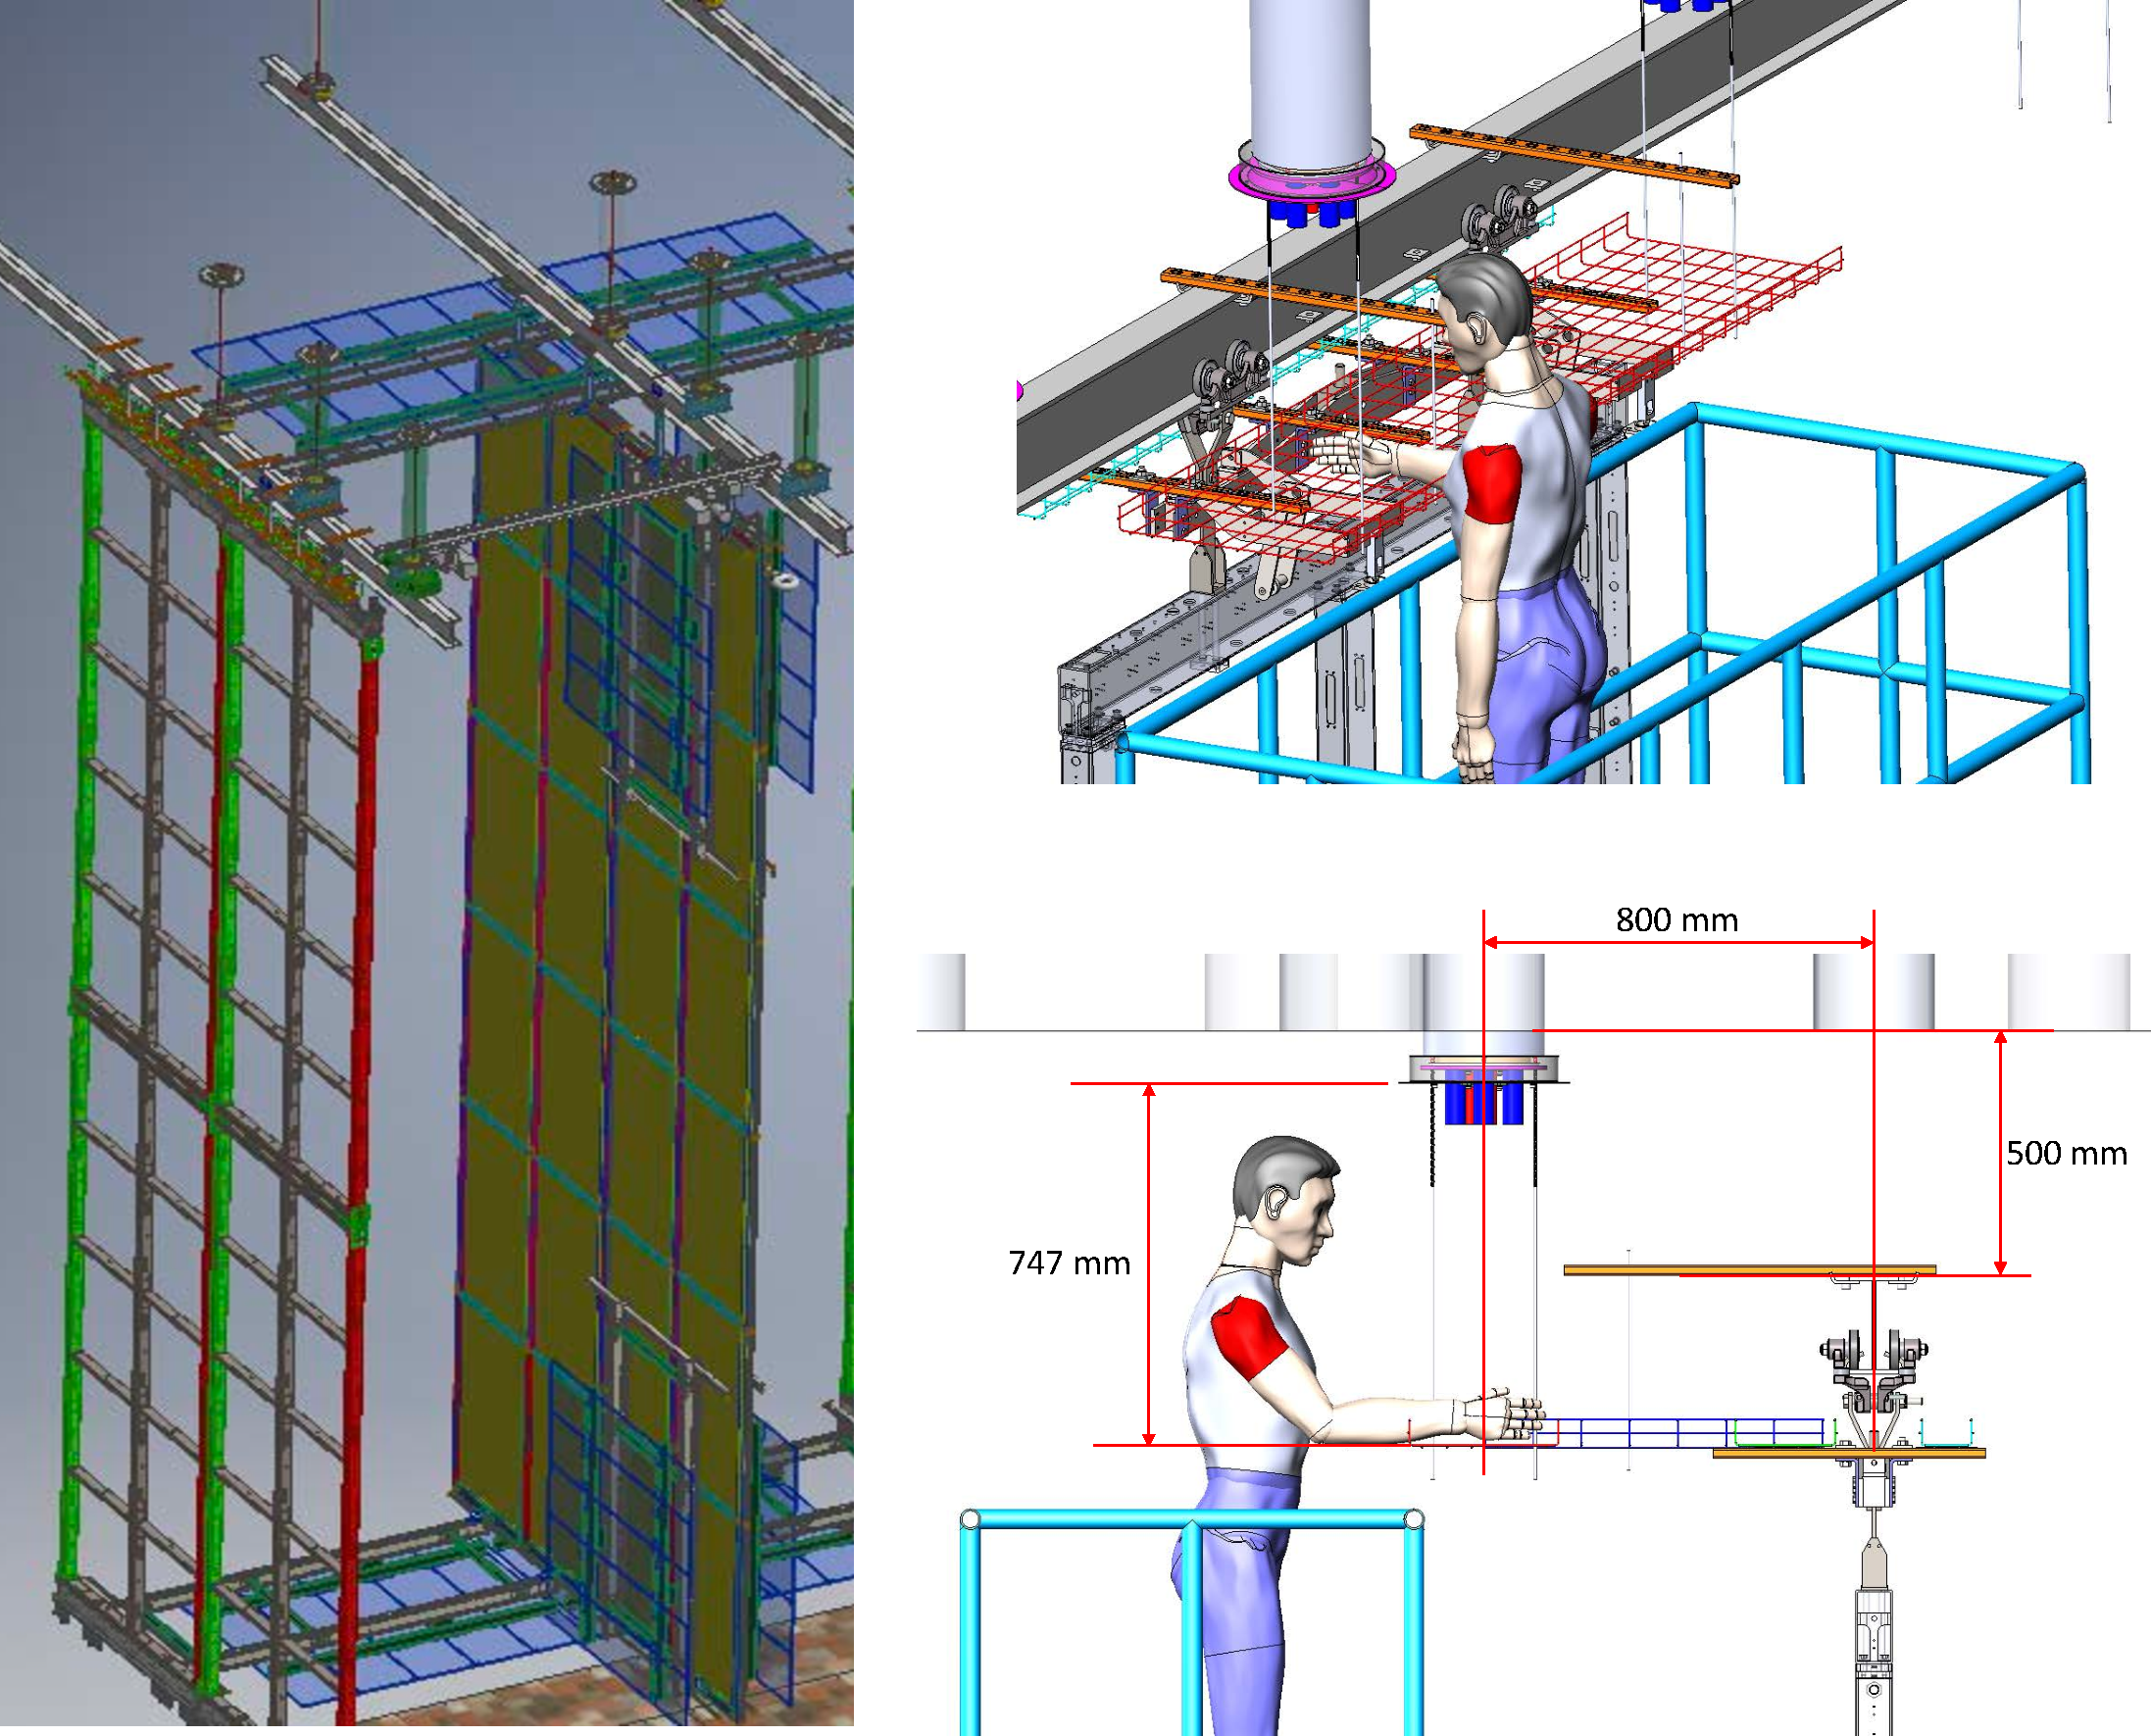
\includegraphics[width=.9\textwidth]{install-ce-cables}
\end{dunefigure}

After the \dword{apa} is moved into position, the permanent support rod is connected to the \dword{dss} beam, and the trolleys are removed. 
The crawler used to push the \dword{apa} along the rails is then moved back through the shuttle area and can be used for the next module. 
After the \dword{apa} is locked into position, the cable tray feedthrough to the \dword{ce} is installed. Now \dword{ce} cabling can start. 
Even when a \dword{cpa} module is already in position, more than 3 \si{m} space remains free between the \dword{apa} and \dword{cpa}, so a scissor lift can easily be positioned in front of the \dword{apa}. 
The two right images in Figure \ref{fig:install-ce-cables} show the situation at the top of the cryostat during cabling. The cables are not shown, so the cable trays and their support infrastructure can be seen. 

When cabling begins, all the cables are in the cable trays. 
A team of two people are in the scissor lift in front of the \dword{apa}, and another team of two people are on top of the cryostat. 
The \dword{ce} cables from the bottom \dword{apa} emerge from the \dword{apa} side-tube and are split into two bundles in the cable tray for a total of four cable bundles. 
The top \dword{apa} also has \dword{ce} cables organized into four bundles. 
The photon cables from both the top and bottom \dword{apa}s are bundled into two cable bundles.
During the cabling process, each bundle is partly removed from the cable tray and then fed up through the cable feedthrough. 
At the top of the feedthrough, the cables are strain relieved, and the cables are also strain relieved at the bottom of the crossing tube.
This is repeated for each of the 10 cable bundles needed for the \dword{apa} pair. 
When all cables are installed through the cable tray, any excess length is returned to the cable tray at the top of the \dword{apa}. 
On the roof, the short individual cables are then connected to the feedthrough flange, and the electronics can be tested. When all electronics and electrical connections are checked, the flange connecting the warm interface crate can be sealed to the cryostat feedthrough flange, and the cable installation is complete. 

Similarly, the \dword{pd} warm cables are connected to the readout module, and the flange sealed after testing.  Once testing is complete, the tray holding the excess cabling is transferred to the \dword{dss} beam.  This minimizes any uneven load on the \dword{apa} pair, so they hang more vertically.   
The electronics for each \dword{apa} is continuously monitored after installation. 

Placing the cables in the cable trays and exactly how the cables are routed is complex. Figure \ref{fig:install-cable-routing} shows the working 3-D model of the cable routing, showing how the cables will be bundled and placed in the trays. A mock up the cabling configuration is planned at BNL, and the installation of the cables will be tested as part of the Ash River testing program.

\begin{dunefigure}[Model of the electronics and photon detector cabling]{fig:install-cable-routing}
  {Working model of the cable trays and routing of the cables in the trays.}
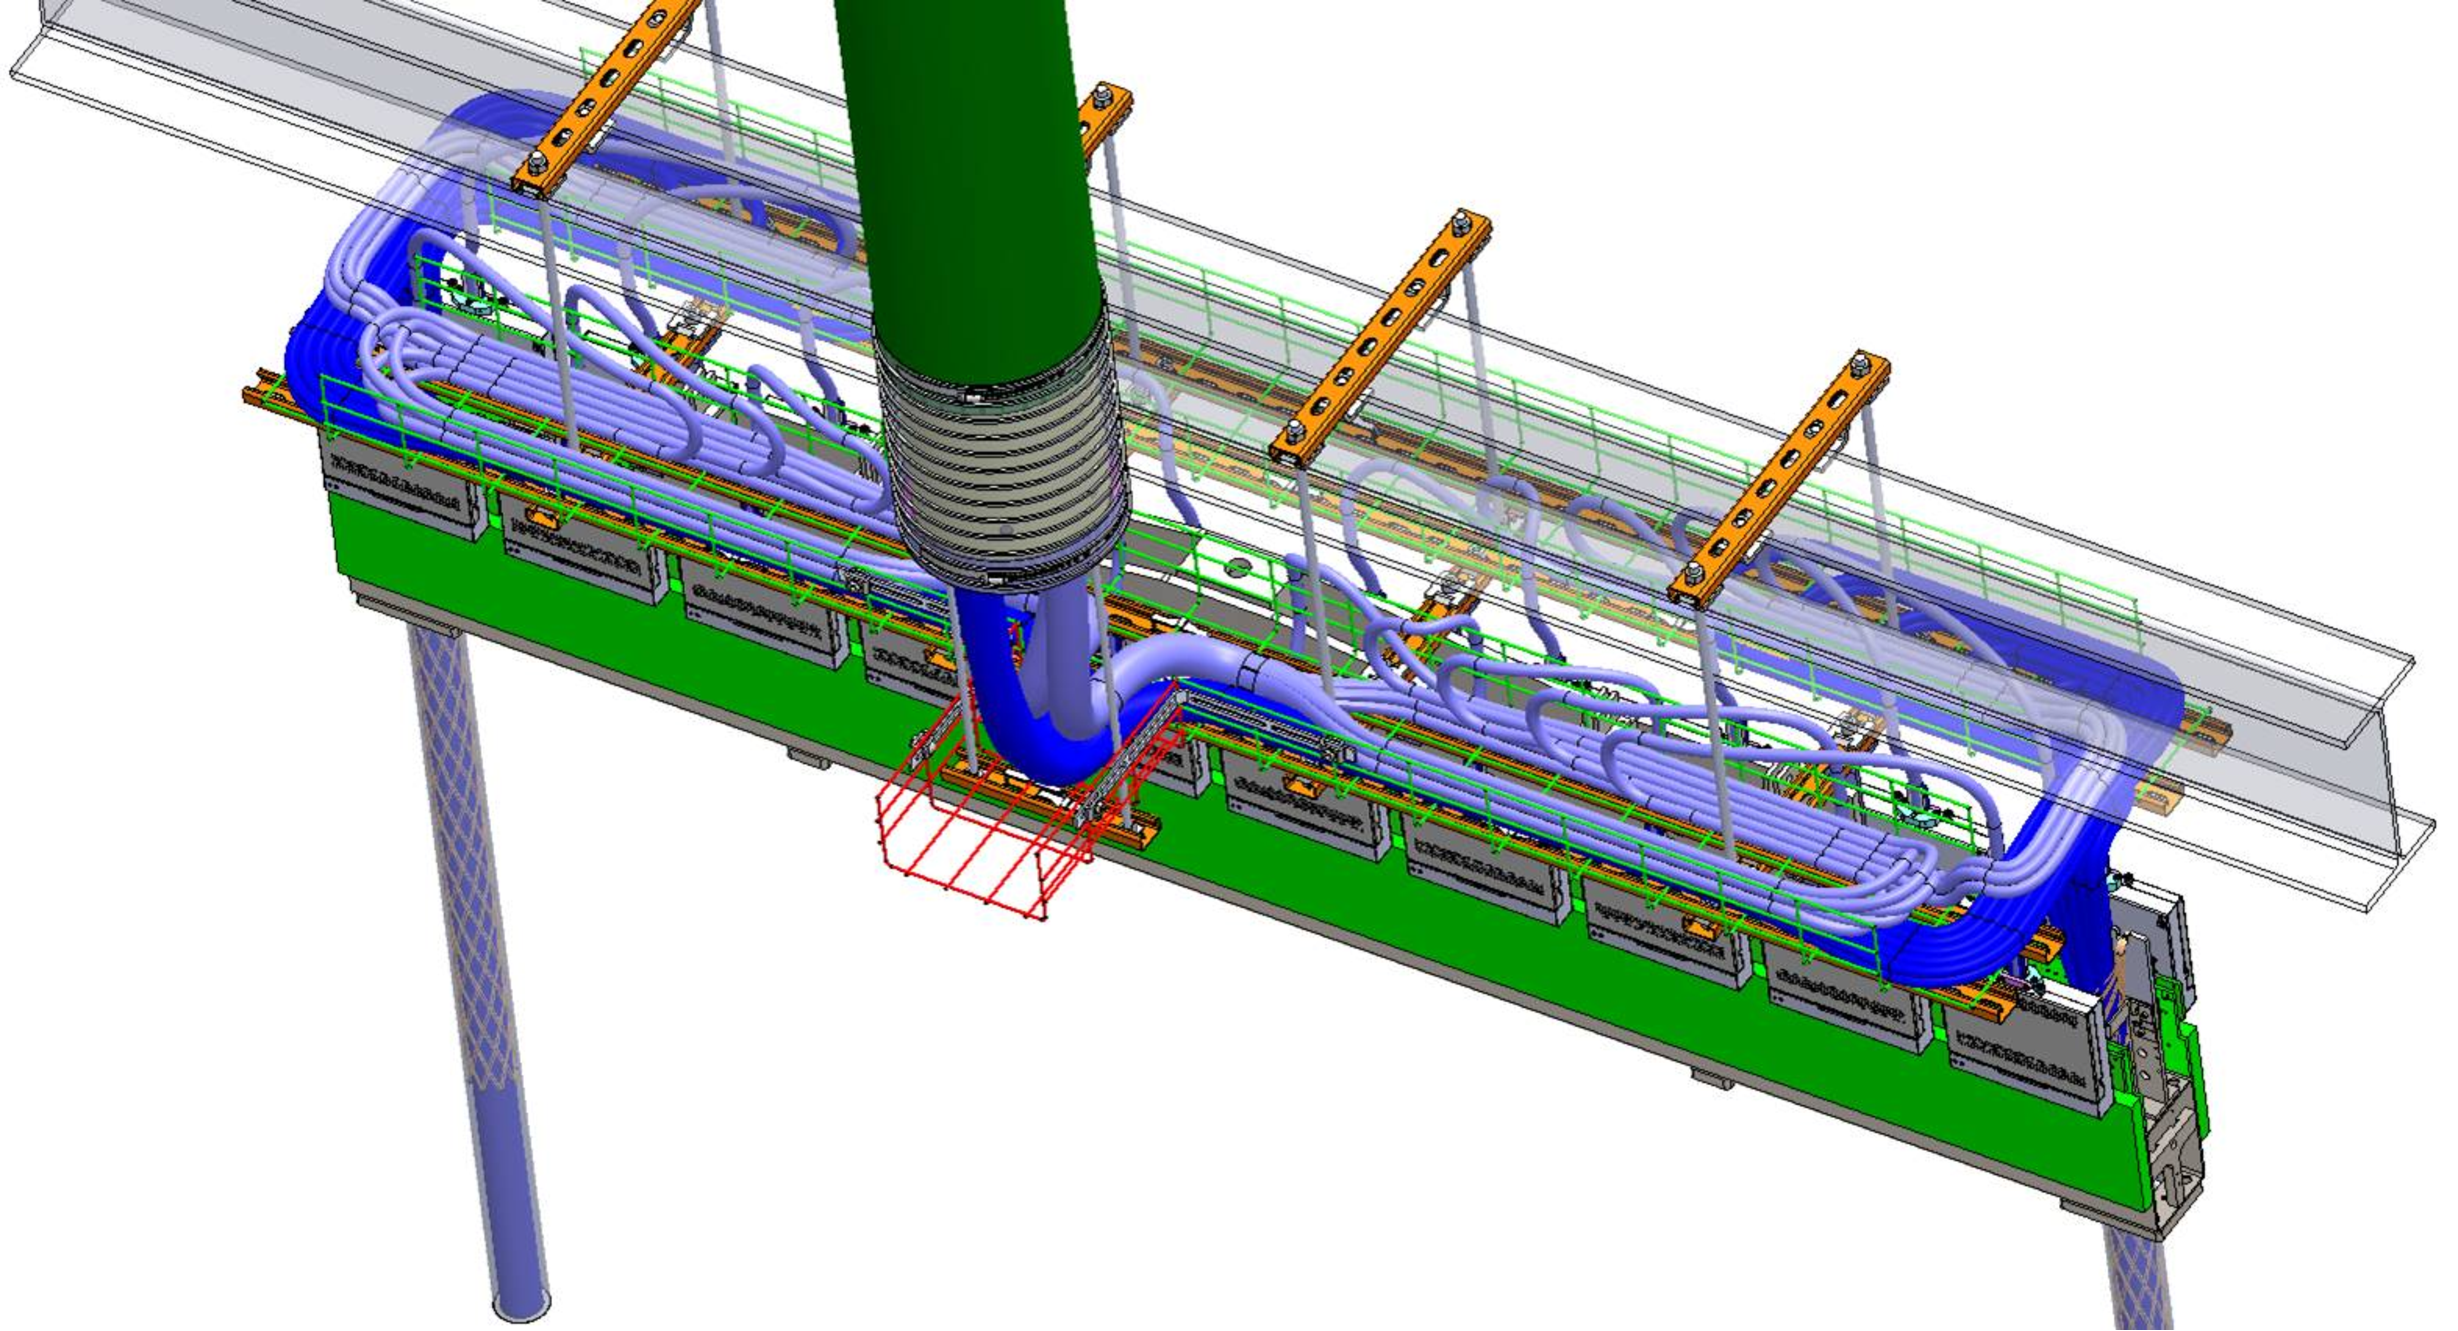
\includegraphics[width=.95\textwidth]{install-cable-routing}
\end{dunefigure}


\begin{dunefigure}[CPA installation]{fig:install-cpa-fieldcage}
  {The top field-cage assemblies are deployed using a custom tool that mounts to the DSS beams as seen in the top left panel. The field cage is lifted using the electric winch controlled by an operator in the nearby scissor lift. The lower field cage is lowered using a hoist mounted on a wheeled frame. The hoist is on a linear slide to keep it aligned above the connection point.}
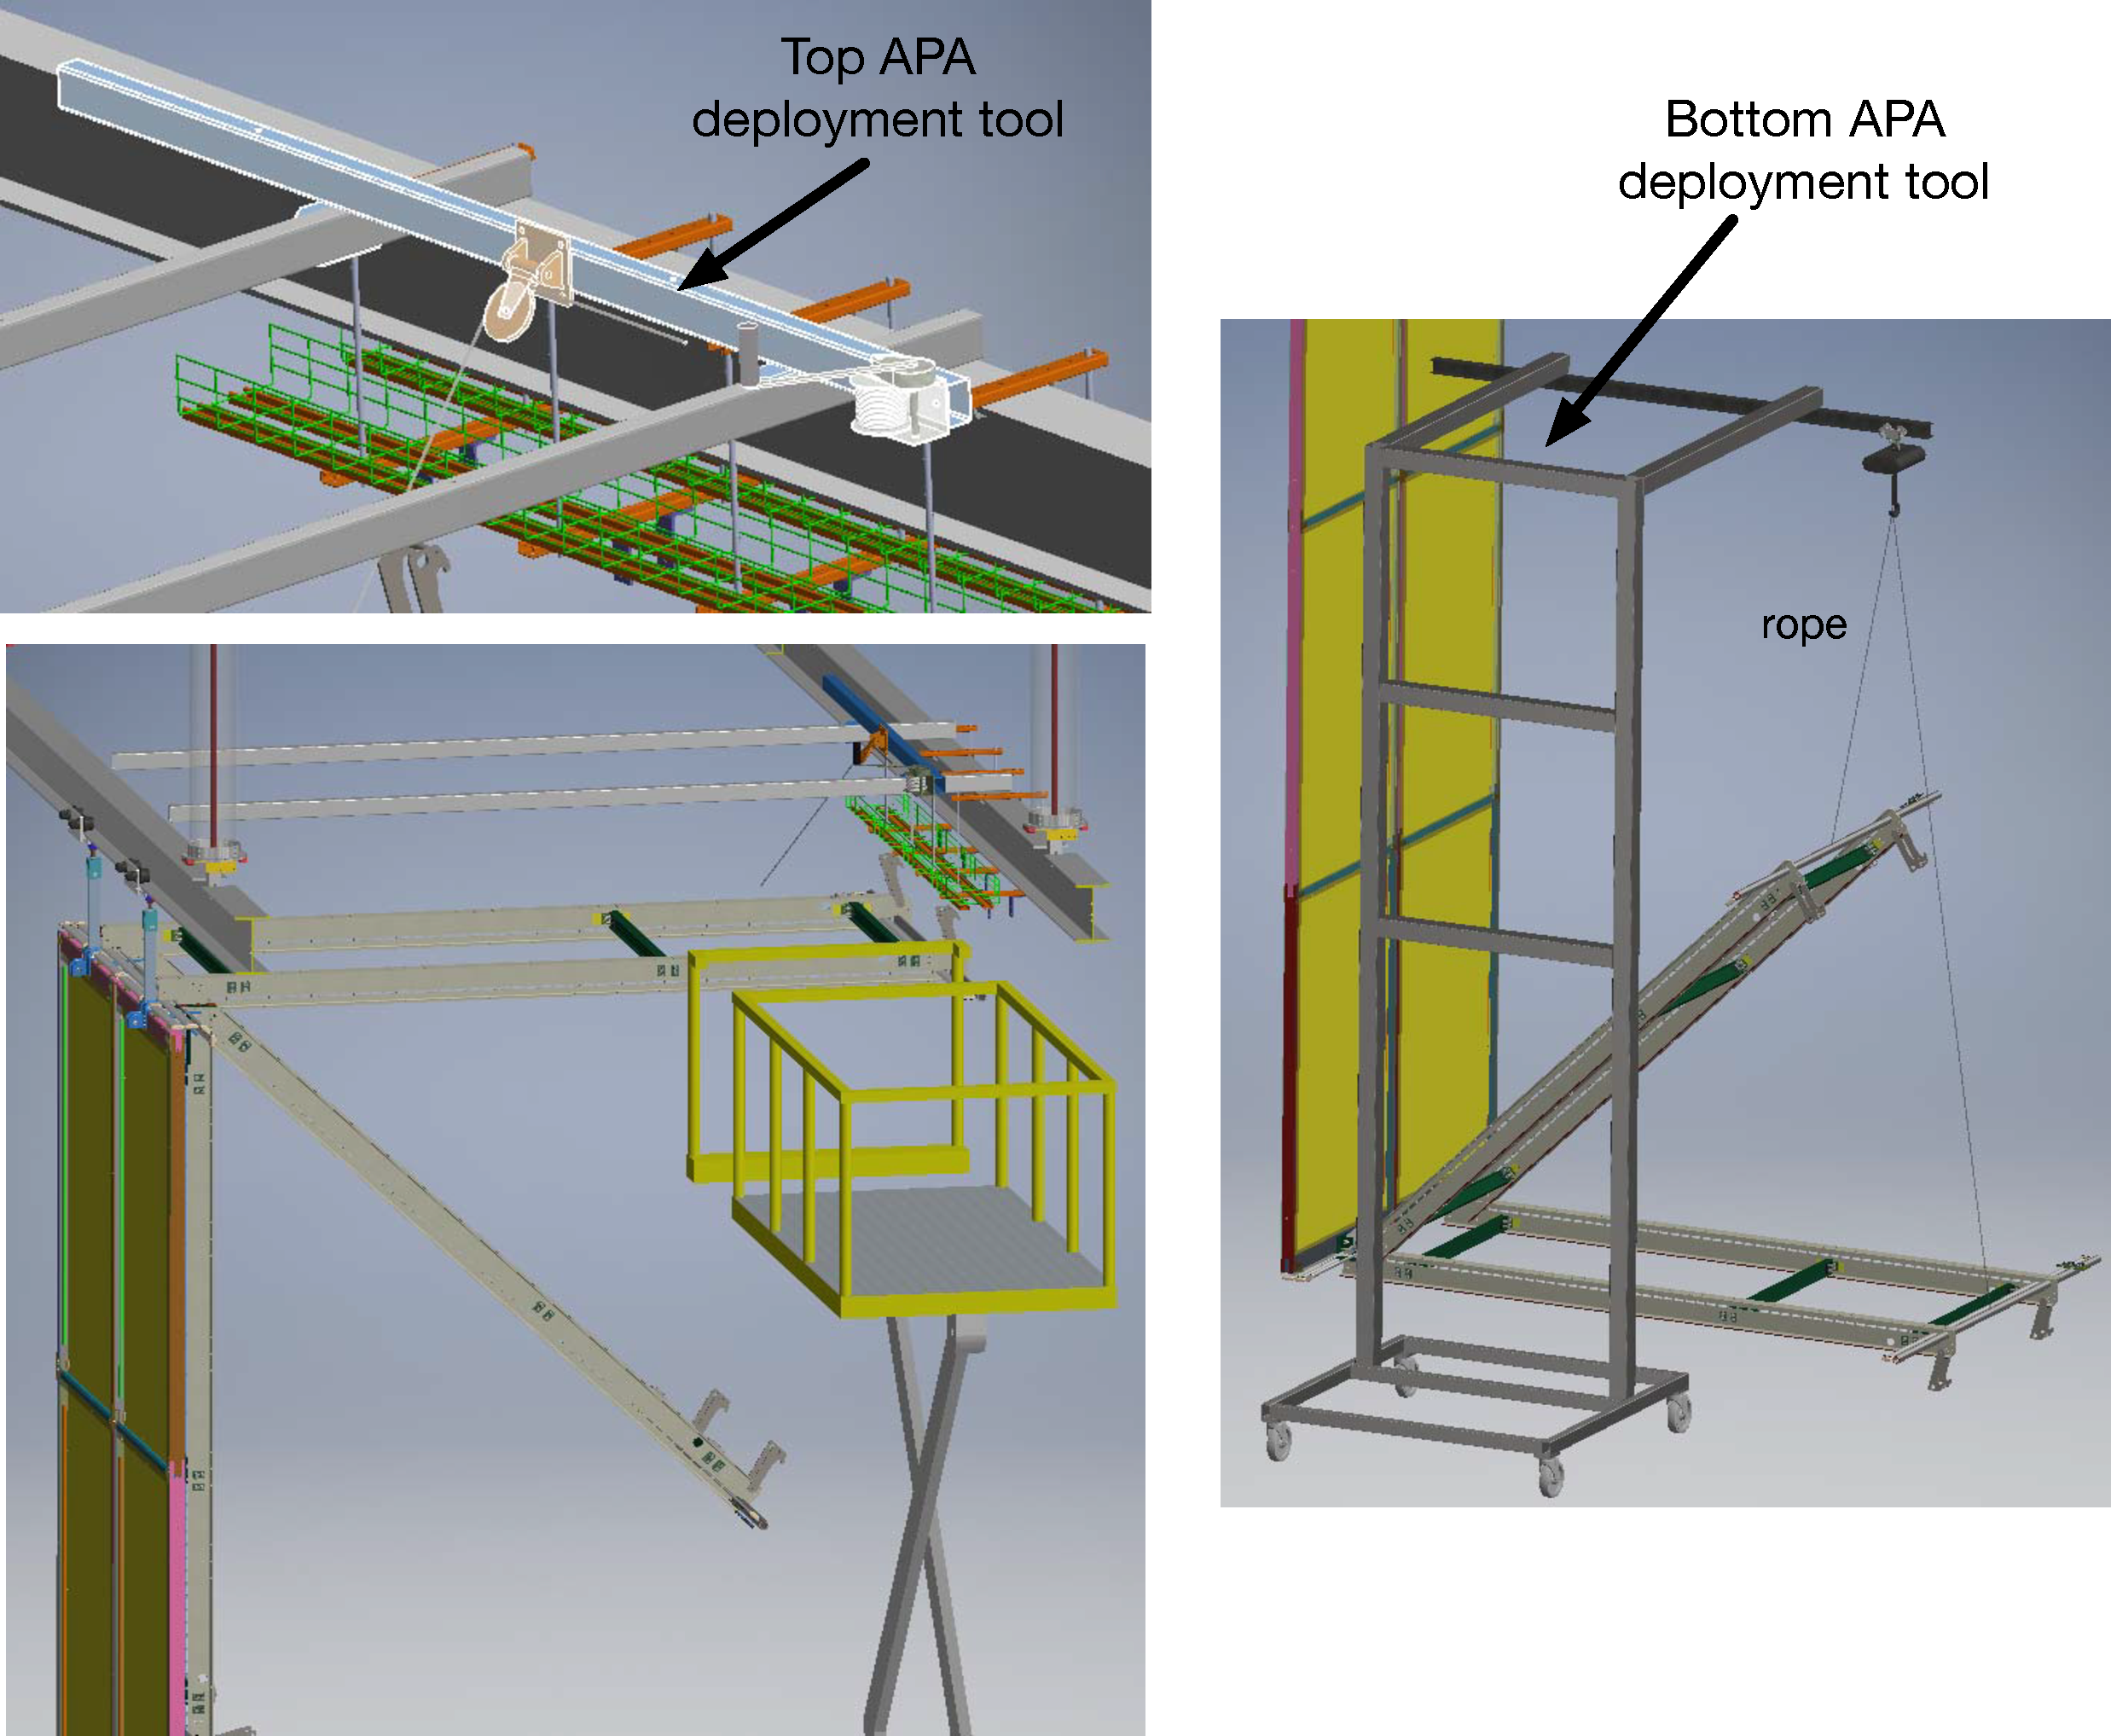
\includegraphics[width=.9\textwidth]{install-cpa-fieldcage}
\end{dunefigure}

The cathode \dword{fc} assemblies are brought into the cryostat like the \dword{apa} pairs, using the overhead rails through the \dword{tco}. Inside the cryostat, they are moved into position using the \dword{dss} switchyard and \dword{dss} I-beams. 
Once in position, the load is transferred to the \dword{dss} beam, and the trolleys are removed. 
The \dword{cpa} will wait in position until its \dword{apa} pairs are fully tested, and then the \dword{fc} modules could be deployed. 
The deployment sequence of the \dword{fc} has not yet been fixed. 
If the \dword{fc} are immediately deployed then the \dword{apa} and \dword{fc} can be tested in the final position. 
If one waits to deploy the field cages then the \dword{ce} can undergo a longer burn in test and the opportunity to clean the cryostat near the end of the installation is available. The decision on the best time to deploy the \dword{fc} will be made closer to the start of installation.
Figure \ref{fig:install-cpa-fieldcage} shows the equipment for deploying the \dwords{fc}. 
The top \dwords{fc} are raised by connecting a cable to the module and then using a pulley-winch assembly to lift the module, which latches to the \dword{apa} mounts. 
A scissor lift is used to connect the cable to the module and also to control the winch. 
After the module is in place, the deployment tool is moved to the next \dword{apa}and \dword{cpa} sets. 
The lower \dword{fc} is deployed using a custom frame that can be wheeled into position. 
The cable from a small host is then attached to the \dword{fc} module, and the module can be lowered. 
The hoist is on a linear slide, so the cable is always directly over the connection point. 
This keeps the \dword{cpa} from swinging because of an induced moment. 
When the module is down, it latches to the \dword{apa} frame much like the upper \dword{fc}. 
The electrical connections to the \dword{hv} bus are tested, and deployment is complete. 
In principal, the cathode/\dword{fc} assemblies can be constructed faster than the \dword{apa}s. 
In theory the cathode/\dword{fc} assembly process could start later than the start of \dword{apa} assembly if the deployment is postponed. 
 The risks and benefits of different deployment sequences will be evaluated near the start of installation.

Periodically during the \dword{tpc} installation the TCO will be temporarily optically closed and the cryostat made dark so the \dword{pd} detectors can be tested. At this time noise measurements will also be performed.

The periscopes for the laser calibration system on the top of the TPC in the center can be installed after the relevant \dword{fc} elements are deployed. The lasers are immediately aligned with the alignment laser system. 
Once for each periscope/laser system, prior to the installation of further TPC components, we will need to clear the cavern to align the UV (Class 4) and visible lasers this will need special safety precautions. 
It may be possible to do this special alignment operation for all lasers at roughly the same time, to minimize the disruption.

\begin{dunefigure}[Installation of row 25]{fig:install-row25}
  {Detector installation as the last row of detector components are installed. At this time, the switchyard beams are removed, and the temporary hoists for the endwall are installed.}
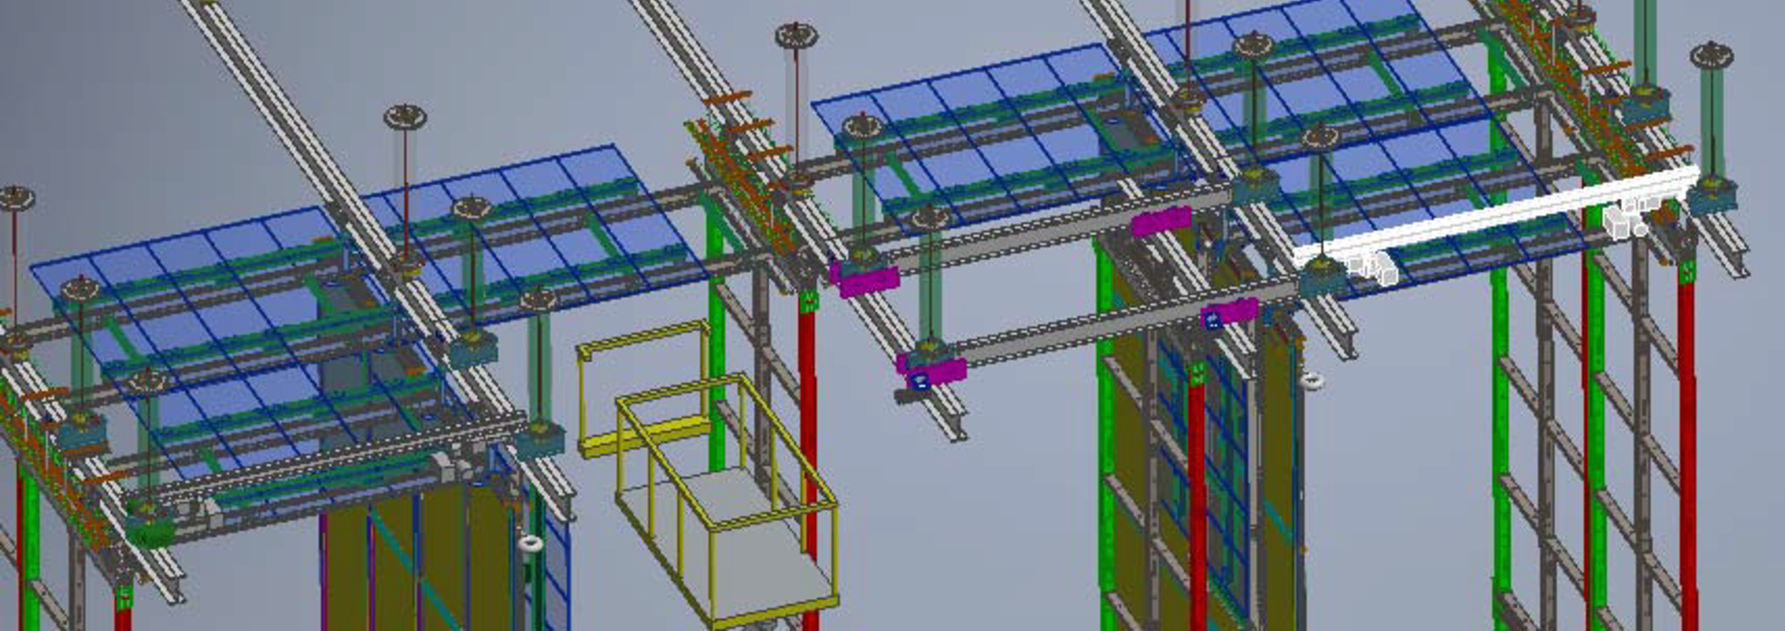
\includegraphics[width=.9\textwidth]{install-row25}
\end{dunefigure}


The last row of detector elements are installed much like previous rows, but the runway beams of the \dword{dss} switchyard are removed as this \dword{apa} and \dword{cpa} are placed in position. Figure \ref{fig:install-row25} shows the top of the detector as this last row is installed. When the shuttle beam is aligned to the correct \dword{apa} or \dword{cpa} row, the short section of the beam is bolted to a short I-beam section of the runway beam that is permanently fixed to the \dword{dss} support feedthrough. When the shuttle beams at both ends of a runway beam section are fixed in position, a section of the runway beam is removed. The last \dword{fc} modules are then deployed. 


\begin{dunefigure}[Second endwall installation]{fig:install-ew2}
  {Installation of the final endwall before closing the TCO.}
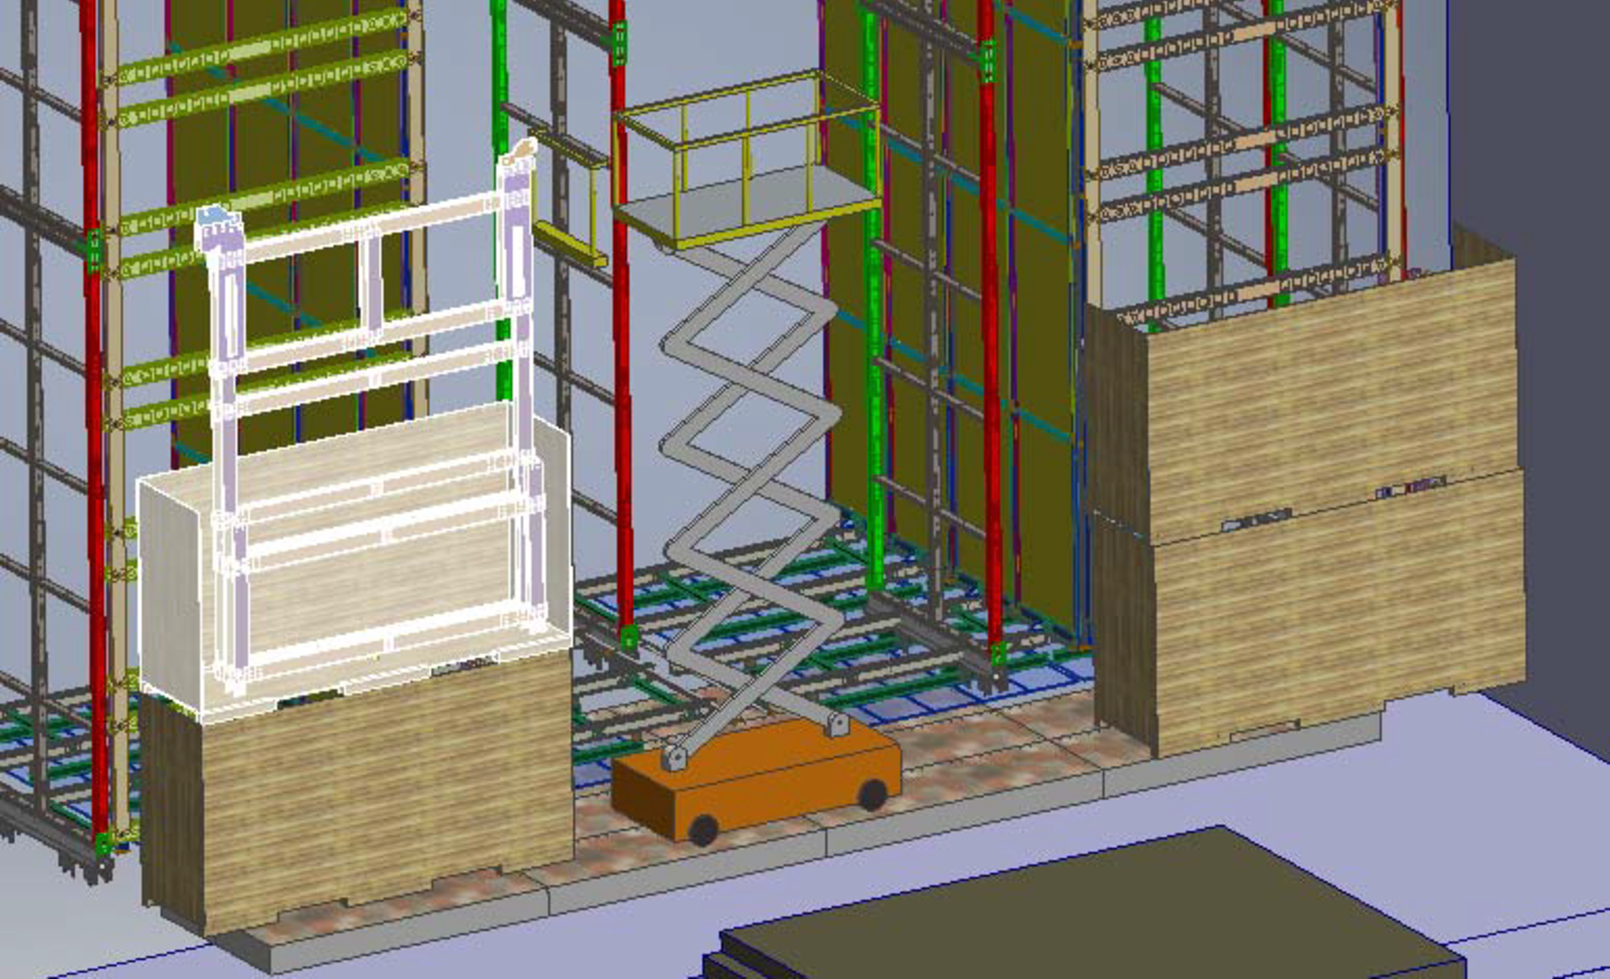
\includegraphics[width=.9\textwidth]{install-ew2}
\end{dunefigure}

The second outside endwall is installed like the first endwall. At this point, the center \dword{apa} is rolled into the cryostat, the shuttle beam is bolted to the \dword{dss}, and the runway beams are removed. The two center drift volumes \dwords{fc} are deployed. The last two endwalls are constructed, and the \dword{tpc} is basically finished. 

At this point, a frame supported by the shuttle beams is covered with flame retardant plastic and installed to create cleanroom work area for the \dword{tco}.  A scaffold is set up for egress to the manhole. The cryostat will become confined space area, so it must be in place before the \dword{tco} is closed.  Closing the top 3/4 of the \dword{tco} is completed using the 14m scissor lift. The temporary cleanroom area is then removed and the area cleaned. A smaller clean area is made to cover the bottom 3.4m \dword{tco} section.  The scissor lift must be removed at this point. The \dword{tco} work is completed and the area cleaned.

A second scaffold is set up in this space  for cleaning and installation of equipment for the calibration and cryogenic instrumentation.

The dynamic T-gradient monitor is installed at this time. 
The monitor comes in several segments with pre-attached sensors and cabling already in place. Each segment is fed into the flange one at a time until the entire sensor carrier rod is in place. The remainder of the system (motor system that moves the sensor rod and the sensors) that goes on top of the flange is installed using a crane. 

The purity monitor system will be built in modules, so it can be assembled outside the cryostat leaving only a few steps to complete inside the cryostat. 
The assembly itself comes into the cryostat with the three individual purity monitors mounted to support tubes that are then mounted to the brackets inside the cryostat. The brackets are then attached to the appropriate elements (cables trays, \dword{dss}, and bolts in the cryostat corner are under consideration). Also at this time, the remaining level monitors are installed.

The periscopes at the end of the detector are installed and aligned. 

Once all this work is completed, the scaffolding is taken apart and hoisted out the man-hole along with all remaining flooring sections. The area is cleaned, and the last two \dword{fte} in the cryostat are hoisted out. 

The inspection cameras and other possible calibration instruments can be installed from the roof while the \dword{tco} is being closed.

After the TCO is closed the manholes can be closed and the pulsed neutron source can be placed in position above two of the manholes. The pulsed neutron source can be tested to confirm neutron yields with integrated monitors and dosimeters in dedicated runs..

% clear the figure buffer before starting the next section
%\clearpage




%%%%%%%%%%%%%%%%%%%%%%%%%%%%
\subsection{Installation Prototyping and Testing (QA/QC)}
\label{sec:fdsp-tc-inst-qaqc}

The section first below describes the planned \dword{qa} process for developing the installation process and qualifying the installation equipment; following this the \dword{qc} planned for the detector installation is described.

\subsubsection{Detector Installation Quality Assurance}

An extensive prototyping program designed to develop and test the \dword{protodune} installation process was executed in the \nova Assembly Area at Ash River prior to the final design of the \dword{protodune} detector. 
The \nova Far Detector Laboratory at Ash River is owned and operated by the University of Minnesota using grants from the DOE and Fermilab.
A mechanical mock-up of one-sixth of the detector was fabricated from test components where the interface infrastructure was considered final. 
Here all the mounting points, external dimensions, loads, latches and hinges were expected to be exactly as planned for the final \dword{protodune} detector.
A fake cryostat roof and wall was constructed to understanding how some tasks could physically be performed in the space available.
Initially all the components failed the installation test and had to be modified. A series of hands on working group meetings with the different consortia were held to resolve installation issues and revise the detector design. 
In some cased two iterations were required before the components could be assembled together in the space available and dedicated tooling had to be developed. 
Having the mock-up of the roof and walls of the cryostat was critical in developing the installation procedures as only when one is physically attempting the work in the space available are all the constraints obvious. 
If the prototype installation test had not been performed the \dword{protodune} would not have been assembled on schedule as many parts would have needed rework.
The experience gained during the \dword{protodune} Ash River trial assembly was critical for both verifying the mechanical design and interface, but also for developing the tools and procedures needed for the installation.
The \dword{dune} \dword{tpc} will have half the available work space  both the above and below the \dword{tpc} inside the cryostat.  
One lesson learned from \dword{protodune} was that access was difficult in this area as the bottom latches were secured and the \dword{apa}s were tied together on the bottom.  
The process of test installing the detector mock-up was where the hazard analysis was refined and detailed procedure documentation for the assembly process was developed. 
Having a detailed well developed hazard analysis was very is important to keep the work on \dword{protodune} safe. Having complete well developed procedures prior to the delivery of the components at CERN allowed the safety approval process to begin early.   The experience at \dword{protodune} showed that testing the installation in advance was necessary in developing the installation plan and insuring that the work can be performed safely. The \dword{dune} installation prototype is also where the time and motion studies can be performed which are required to develop a reliable schedule.

Mechanical tests at the \dword{dune} trial assembly at Ash River will be key to developing the installation process, but other important prototyping tasks performed at other universities, national laboratories, and CERN also are needed to develop the installation plan. 
For example; Argonne National Laboratory is testing the \dword{apa} shuttle beam drive system and the \dword{cpa} assembly tower connections before they are shipped to Ash River.  
Brookhaven National Laboratory is planning a test setup to develop the cable management process on top of the detector.
Many small steps in the assembly process have been improved using our past experience at CERN and will be developed further during this prototyping phase. 


\begin{dunefigure}[NOvA Assembly Area at Ash River]
{fig:NOvA-Assembly-Area}
{Top Panel shows the \nova Assembly Area and the bottom panel shows the 3-D model of the installation prototype.}                
%\centering     %trim=left bottom right top, clip
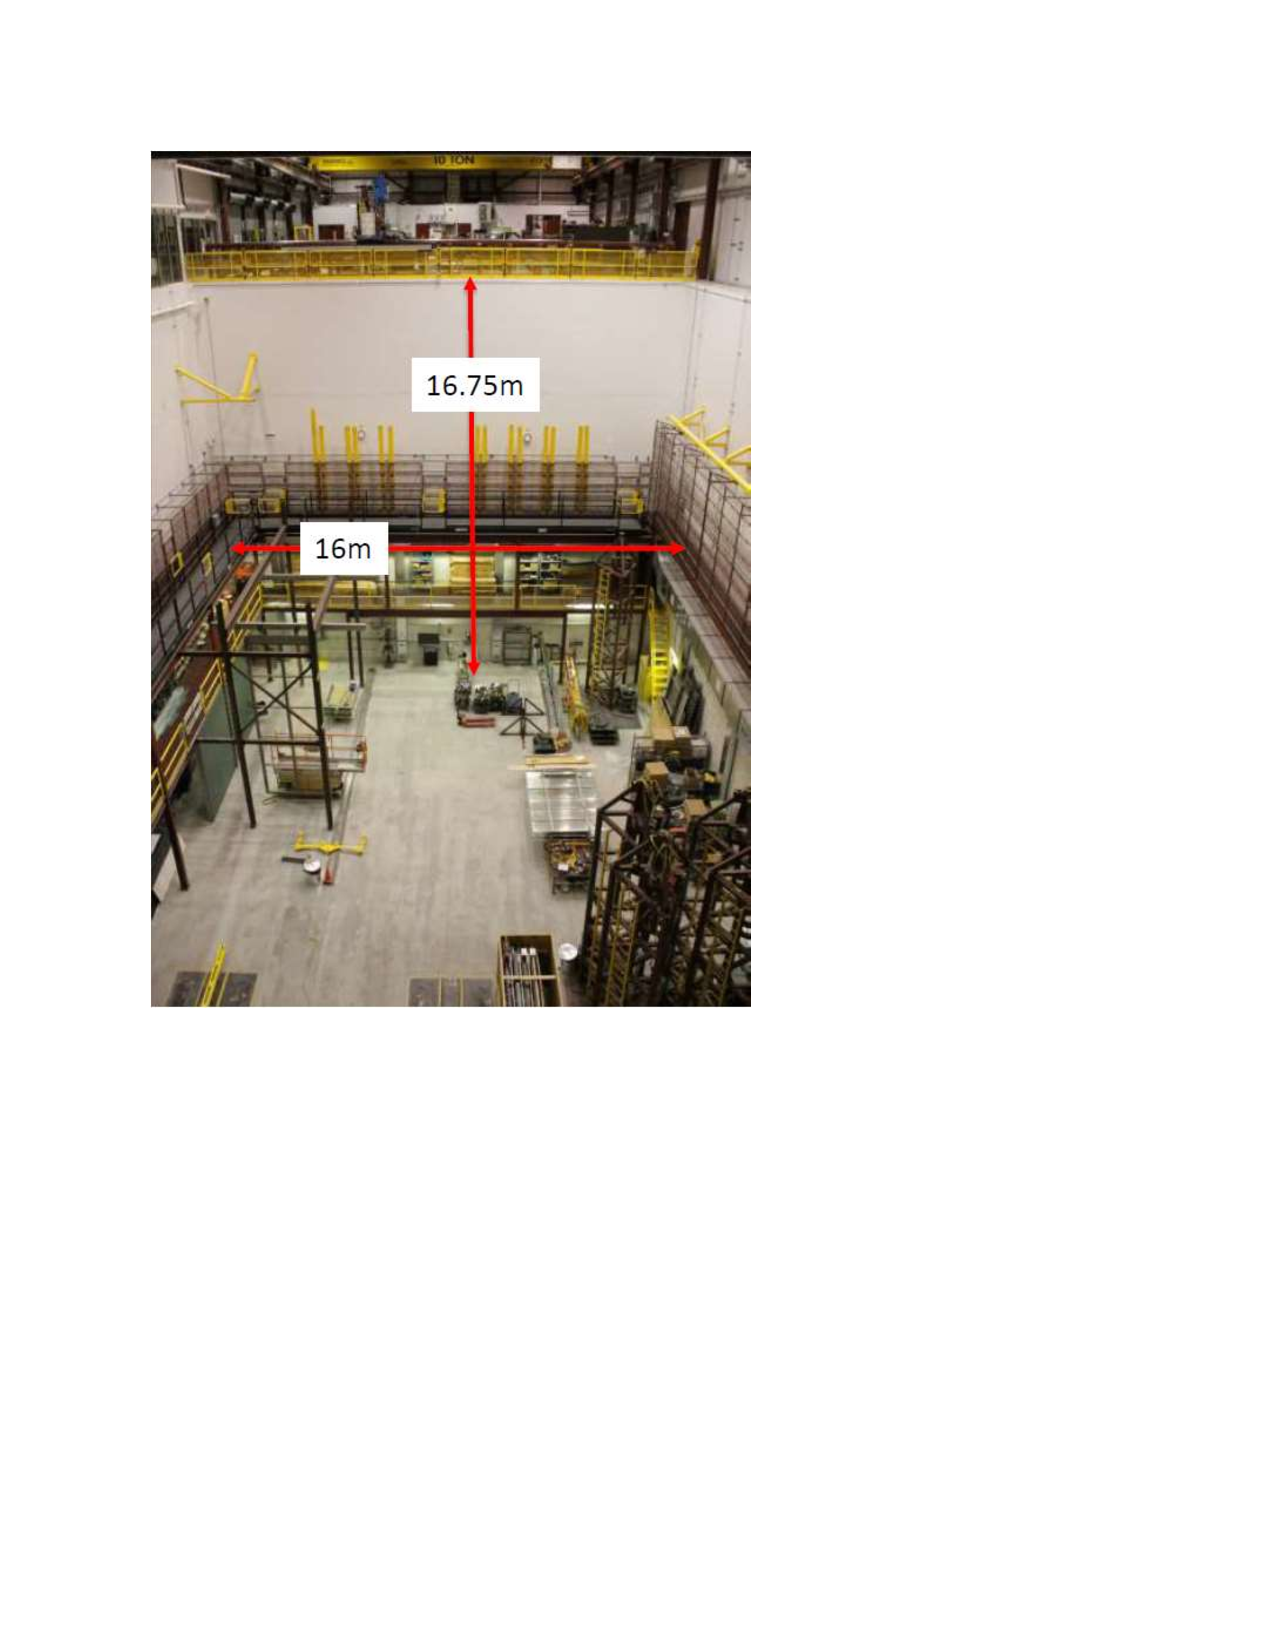
\includegraphics[width=0.49\textwidth]{NOvA-Assembly-Area}
\vspace{-12pt}
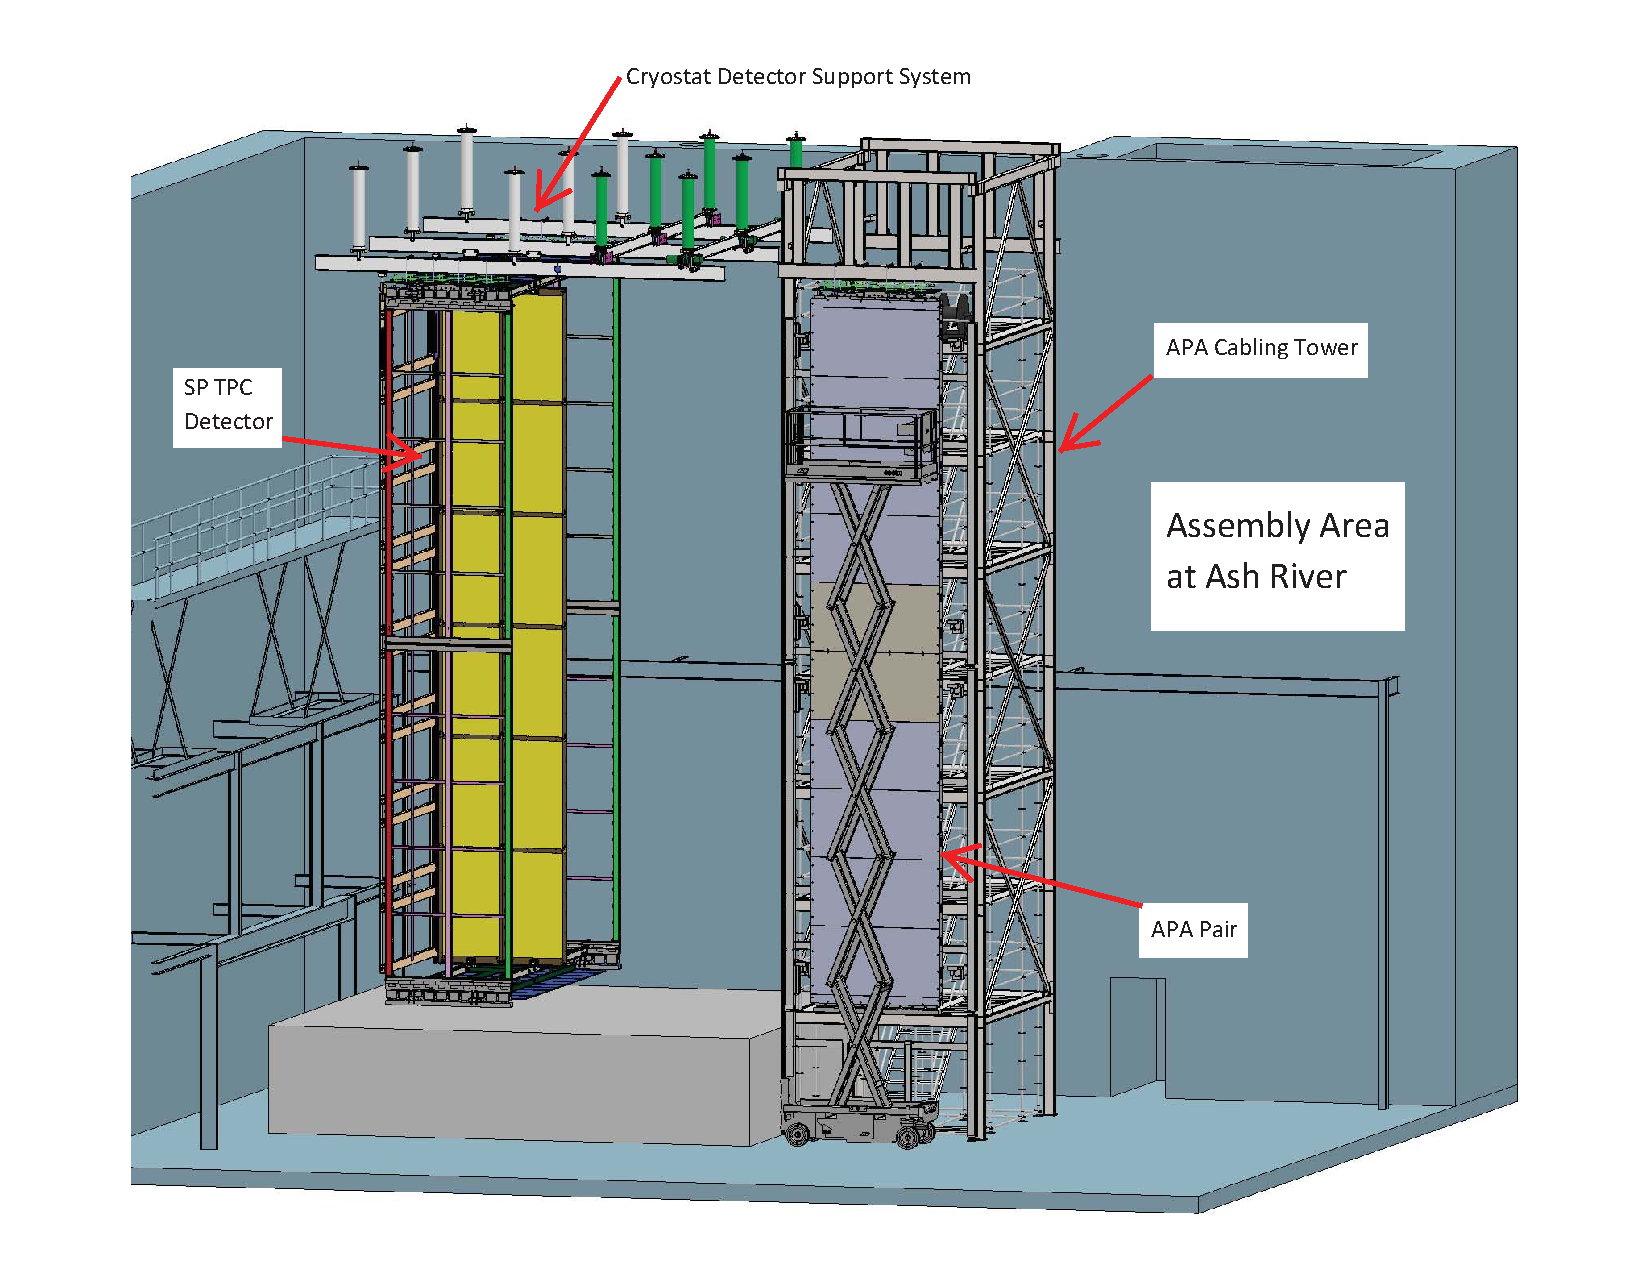
\includegraphics[width=0.8\textwidth,trim=0pt 0pt 0pt 0pt,clip]
{DUNE-Trial-Assembly-Ash-River}
\end{dunefigure}

Full scale mechanical testing of the assembly and installation of all the \dword{tpc} components, including the \dword{dss}, will be critical for the success of the single phase detector as shown from the \dword{protodune} prototyping experience. 
To achieve the same success in \dword{dune}, a prototype of the installation
equipment for the \dword{spmod}  will be constructed at the \nova neutrino experiment \dword{fd} site in Ash River, Minnesota, USA, and the installation process tested with dummy detector elements.  
The \nova Far Detector assembly area at Ash River, shown in Figure \ref{fig:NOvA-Assembly-Area}, meets the requirements of both area and available equipment as well as having experienced technicians that helped construct the \dword{protodune} detector. 
The \nova Far Detector assembly area (see Figure~\ref{fig:NOvA-Assembly-Area}) has both the elevation and floor space available to do a full-scale test of both the component assembly outside the cryostat and a test installation of the \dword{tpc} components  inside of the \dword{dune} cryostat. 
At Ash River,  a 75 \si{ft} $\times$  100 \si{ft} loading dock and ramp access, two 10-ton cranes, a machine shop, and wide assortment of tools are also available.  Add the experienced crew of technicians who all had several months at CERN building \dword{protodune} as well as fabricating experience and Ash River is the obvious place for the \dword{dune} installation prototyping exercise. 

While the University of Minnesota has jurisdiction over the safety program at Ash River, we also follow the Fermilab Safety Program and work together to ensure a safe working environment.  
One key attribute of the \dword{protodune} work was compiling sets of documentation from component design to hazard analysis to final assembly procedures for approval by the CERN Health Safety and Environment division. 
For Ash River and \dword{dune}, this is all part of the Operational Readiness Clearance (ORC) review process. 
Documentation for both the trail assembly process at Ash River and for \dword{dune} will be stored on the \dword{edms} at CERN. 
Though many of the \dword{tpc} components are mechanically similar to the \dword{protodune} components, the access equipment will be different and the need to work at \SI{14}{m} height will make construction of the \dword{dune} single phase detector much more challenging.  


The \dword{dune} \dword{fd} trial assembly program at Ash River has the following goals:

\begin{enumerate}
\item Validate the \dword{apa} design. 
\item Test all full scale \dword{tpc} components during both the initial assembly stages in the cleanroom outside the cryostat and the deployment stages inside the cryostat:  
\begin{itemize}
    \item \dword{apa}  assembly: manipulation of \dword{apa} shipping frames, joining an \dword{apa} pair together, \dword{ce} cabling, removal and re-installation of the \dword{apa} protection covers, movement on shuttle beam, cryostat cabling, and final deployment in cryostat. 
    \item Integration and installation testing of \dword{pd} (Photon Detector) components: cable harness routing and cryogenic cable strain relief, module integration into \dword{apa} frames, and electrical connections between upper and lower \dword{apa}s.  In addition, \dword{pd} monitoring system components mounting and optical fiber routing on the \dword{cpa} will be tested.
    \item \dword{dss} and shuttle beam system, including final detector configuration.
    \item Assembly of \dword{hv} system: construction of an endwall, \dword{cpa} pairs, movement on shuttle beam, and final deployment in cryostat.
\end{itemize}
\item Write full set of hazard analyses and assembly procedure documents, including gathering all component documentation. 
\item Test access equipment (scaffold, scissor lifts, work platforms) and lifting fixtures. 
\item Study assembly time and motion, including labor estimates. This facility can also be used as a training site for lead workers as \dword{dune} begins set up and for testing mechanical modifications.
\item Train the installation team prior to the start of \dword{dune} installation. 
\item Possible future assembly tests of the dual phase detector components.
\end{enumerate}


In order to meet the above goals a staged testing program has been developed.  The initial phase is dedicated to qualifying the \dword{apa} and \dword{fc} designs. The main difference (other than the number of units) between \dword{protodune} and  \dword{dune} is that the \dword{dune} detector is twice as tall. This is achieved by hanging one \dword{apa} beneath another. Unfortunately the \dword{apa} built for \dword{protodune} were not designed for this so the cables from the lower \dword{apa} could be routed through the upper \dword{apa} thus requiring a major redesign. To date a pair of \dword{apa} has never been assembled or cabled. The handling of the lower \dword{apa} and the assembly into a double has also never been tested. As shown in \dword{protodune} these tests are critical and must be completed before the design of the \dword{apa} is final. The initial phase of the installaiton testing is focused on this and is time critical as the work must be complete before \dword{apa} production can begin in 2020. In parallel to the dword{apa} testing the assembly of the \dword{cpa} and the deployment of the \dword{cpa} can also be tested as they will not require large amounts of additional infrastructure.

The second phase of the prototyping program is focused on developing the installation plan and verifying all the detector interfaces are correct. Here a full scale model of the major equipment in the cleanroom and inside the cryostat is constructed. A dry run of the assembly, component transport and deployment in the cryostat can then be performed. This is especially important as the space in the cryostat is above and below the detector is half that of \dword{protodune} where some of the installation steps were already challenging.

The final stage includes a mock-up of the top of the cryostat so the final cabling steps can be tested at height. With this setup accurate time and motion studies can be performed to bench mark the installation schedule. Detailed procedures can be drafted and in place before the start of actual installation. Also the installation team can be trained prior to work underground. 

By testing the installation process early all the hazards can be identified and remediation implemented. It is important to have an excellent understanding of the hazards associated with the underground work in advance so measure can be implemented to reduce risk. The prototyping effort provides a means to identify the hazards and develop engineering measures to reduce the risk without the time pressure associated with the actual installation. Remember by definition, detector installation  is on the critical path, making it vital that the work be performed efficiently and with the lowest possible risk. 

This prototyping program is summarized in Table \ref{tab:AR-test-program} and the 3-D model representing the final layout is shown in Figure \ref{fig:NOvA-Assembly-Area}. 

\begin{dunetable}
[Summary of the tests at Ash River]
{p{.2\textwidth}p{.7\textwidth}} %{ll}
{tab:AR-test-program}
{Summary of the tests at Ash River} 
Testing phase & Deliverables\\ \toprowrule
FY-19 20 Phase 0   &  \\ \colhline
 & Build an APA cabling tower for full scale APA pair assembly \\ \colhline
 & Check vertical cabling with a pair of APA side tubes \\ \colhline
 & Test APA shipping frame and underground handling\\ \colhline
 & Build a CPA assembly stand and test assembly process \\ \colhline
 & Test FC deployment and ground plane installation \\ \colhline
  FY-20 21 Phase 1 &  \\ \colhline
  & Build support structure for DSS shuttle, 3 sections of DSS beam \\ \colhline
  &  Test movement of CPA and APA from cleanroom to final destination\\ \colhline
  & Test APA, CPA, Endwall and FC deployment in one drift section \\ \colhline
  & Test assembly sequence of final section of TPC \\ \colhline
  & Removal of DSS shuttle beam runway rails \\ \colhline
  & Final deployment after TCO is closed up \\ \colhline
  FY-22 thru FY23 Phase 2&  \\ \colhline
  &  Include the top of the cryostat ( no warm structure) with \fdth \\
  \colhline
  & Test DSS installation  \\  \colhline
  &  Test CE cable installation using \fdth \\  \colhline
  & Design \fdth to support Dual Phase installation test \\ \colhline
  & Test shipping and construction using first factory TPC components  \\ \colhline
  & Train lead workers for underground at SURF \\ \colhline

\end{dunetable}



The testing and quality control measure taken during the installation will now be described.


\subsubsection{DAQ QC testing}

Testing is required at several stages of \dword{daq} installation.  The first is the installation of the dataroom infrastructure, where cooling water leak checking, rack airflow, and power distribution will be tested upon installation by professional data center building contractors.

The detector-to-dataroom multimode fiber will run close to its optical power budget.  This fiber is routed from the \dwords{wib} on top of the cryostat to the servers in the \dword{cuc}, so it must be installed and tested by fiber professionals early in the process.  Covered cable trays will protect it after installation.  As \dword{apa}s and servers are commissioned, pre-tested fibers will be connected to the newly installed hardware.

The \dword{daq} servers in the \dword{cuc} dataroom will be initially received and integrated off site.  Upon installation in the \dword{cuc}, only a simple functionality test will be needed.  Sufficient spare capacity will be installed, and the main commissioning work will be software related and can be done over the network from the surface or remotely.

\subsubsection{APA QC testing}

After the \dword{apa} transport boxes are brought into the material airlock the outer covers are removed and a visual inspection can be performed. Next the \dword{apa} are moved to the \dword{pd}, tests here are described in the \dword{pd}  section.

When the \dword{pd} integration is complete the \dword{apa} transport box is moved to one of \dword{apa} assembly lines. Individual \dword{apa}s are removed from the transport frame, mounted to the assembly line rails, and the protective covers removed. A second detailed visual inspection is performed now the the wires are visible. A spot check of the wire tensions will verify that there has been no change since the \dword{apa} left the factory.
Ideally, all wires would be measured, but time is not sufficient. 
In the current plan, the tension measurements are performed using a laser focused on individual wires, the same method used at the production site. 
The wire is plucked to induce a vibration, and a photodiode under the wire records the frequency of vibration, which directly translates into the tension value. 
The measured values are stored in the wire \dword{dcdb} database. 
While this method is robust and has been extensively used by \dword{lartpc} experiments, it is very time consuming. 
Two people over three shifts will be able to measure approximately 350 wires, 10\% of the total.  An alternative method, using electrical signals, is currently under development and could replace the laser method, potentially allowing measurement of all the wires in less time.
The current requirement for tension values are 6$\pm$1 N, however this tolerance is currently under study with \dword{protodune} data.  
Wires measuring outside the final tolerance will be removed from the \dword{apa}.
\dword{apa} wires are also tested for continuity, to make sure they are intact and properly connected to the readout boards.
This test is done as part of the \dword{ce} testing below. 
Photogrammetry is used to measure the final assembled dimensions of the \dword{apa} either while the wire tension is being measured or immediately before entering the \coldbox.

Once the \dword{apa}s have been installed the \dword{ce} will be continuously read out which will directly inform wire continuity and the full function of the channels. 

\subsubsection{CE QC Testing}


\fixme{Jim's attempt to describe the installation QC for CE (Anne removed the part that's done before arrival in SD 4/8)}

Before arriving in South Dakota all \dword{femb} have been tested both warm and cold, the \dword{wec} are assembled and tested. 
All electronics is shipped in ESD bags or containers. \dword{esd}
All Personnel follow ESD proceedures during installation.
The \dword{wec} are installed first as they can be installed after the cryostat crossing tubes are installed. The\dword{wec} can then be tested stand alone from a laptop. 
When the \dword{femb} arrive underground they are again tested to verify that no damage in transit occurred.
The \dword{femb} are again tested after they are mounted on the \dword{apa} and the final cables are attached. This warm test verifies that nothing was damaged as they were installed on the \dword{apa} and the data is also used to verify that there is continuity along the wires in the \dword{apa}.
The next testing step is the cold test in the \coldbox. 
This test is critical as it verified that there are no connections that open up during thermal cycling and as the \coldbox{}s are Faraday cages the noise levels both warm and cold can be measured. 
Finally after the \dword{apa} is installed and cables in the cryostat it is readout continuously to make sure there are no failures over a significant burn in period. 
It is planned at several times during the installation to temporarily close the TCO to allow noise measurements under controlled conditions.
The measurements will continue after the TCO is closed permanently.


\subsubsection{\dword{hv} QC testing}

The endwalls are assembled in eight panel units, four on each end of the \dword{tpc}.  
As each of the eight panels are removed from the shipping crate and placed on the installation cart, the endwall panel checklist is filled out.\cite{bib:docdb10452}
This checklist includes a visual inspection of the frames, profiles, and connections, as well as continuity and resistance measurements of the divider boards and their connections.  
After completing an eight panel endwall in the cryostat, the complete endwall checklist is filled out.  
This includes hanging position, straightness measurements, and continuity checks between panels.

The \dword{cpa} panels are assembled from three units removed from the shipping crates.  
After each unit is removed from its bag, a visual inspection confirms structural integrity and the connections between \dwords{fss}, \dword{hv} bus pieces, and profiles if present.  
After inspection, the unit is positioned on the \dword{cpa} assembly tower.  
After all three units are connected on the tower, the \dword{cpa} panel checklist is filled out.  
This includes inspecting all mechanical connections, continuity checks of the \dword{fss}, \dword{rp}, profile, and \dword{hv} bus connections, and resistance measurements of the four mini-resistor board connections from the \dword{rp} to the \dword{fss}.  
This is repeated for the second panel in a \dword{cpa} plane.  Then the two panels are paired, each hanging from trolleys on the transport beam.  
Visual inspection of the alignment and hanging straightness are made and \dword{hv} bus connections at the top and bottom are made and checked for continuity (\dword{cpa} plane checklist).

The \dword{fc} top and bottom units are removed from their crates.  The \dword{fc} unit checklist is filled out with a visual inspection of the frames, profiles, and connections, as well as continuity and resistance measurements of the divider boards and their connections.  
After hanging the top \dword{fc} units on the \dword{cpa} plane, the four jumpers from the first \dword{fc} profile on each side of the \dword{cpa} and the \dword{cpa} \dword{fss} is connected, and the resistance is measured, completing the \dword{cpa}/\dword{fc} top assembly checklist. 
The \dword{fc} bottom units are not attached to the \dword{cpa} but are taken into the cryostat independently after filling out the \dword{fc} unit checklist.

The \dword{cpa}/\dword{fc} top assembly is moved into its position in the cryostat.   
After deploying the \dword{fc} top units, the resistor board/jumper between the \dword{fc} and the \dword{cpa} \dword{fss} are visually inspected.  
Also, the latch at the \dword{fc}/\dword{apa} is visually inspected.  After deploying the \dword{fc} bottoms, visual inspection verifies the resistor board/jumper connection from the \dword{fc} to the \dword{cpa}.  
Also, the latch connecting the \dword{fc} bottom to the \dword{apa} is visually inspected.  
These are included in the \dword{cpa}/\dword{fc} cryostat checklist.



\subsubsection{CISC QC testing}

Cryogenics instrumentation systems must undergo a series of tests to guarantee they will perform as expected: 

\begin{itemize}
\item {\bf Purity Monitors}: Each of the fully assembled purity monitor arrays is placed in its shipping tube, which serves as a vacuum chamber to test all electric and optical connections at \surf before the system is inserted into the cryostat. During insertion, electrical connections are tested continuously with multimeters and electrometers.

\item {\bf Static T-gradient Thermometers}: Right after each sensor array is installed, its verticality 
is checked, and the tensions in the stainless steel strings adjusted as necessary. Once cables are routed to the corresponding \dword{dss} ports, the entire readout chain is tested. This allows a test of the sensor, the sensor-connector assembly, the cable-connector assemblies at both ends, and the noise level inside the cryostat.
If any sensor presents a problem, it is replaced. If the problem persists, the cable is checked and replaced as needed.

\item {\bf Dynamic T-gradient Thermometers}: The full system is tested after it is installed in the cryostat. Two aspects are particularly important: the vertical motion of the system using the step motor, which is controlled through the slow controls system, and the full readout chain, which will be tested mainly for failures in sensors, cables, and connectors inside the cryostat. 

\item {\bf Individual Sensors}: To address the quality of individual precision sensors, the same method is used as for
the static T-gradient monitors. For standard \dwords{rtd} to be installed on the cryostat walls, floor, and roof, calibration is not an issue. Any \dword{qc} required for associated cables and connectors is performed following the same procedure as for precision sensors.

\item {\bf Gas Analyzers}: Once the gas analyzer modules are installed at \surf and before the cryostat is commissioned, the analyzers 
are checked for both \textit{zero} and the \textit{span} values using a gas-mixing instrument and two gas cylinders, one with a
zero level of the gas analyzer contaminant species and the other with a known percentage of the contaminant gas. This verifies that the gas analyzers are operating properly. 

\item {\bf Liquid Level Monitoring}: Once installed in the four cryostat corners, the capacitive level meters are tested in situ 
using a suitable dielectric in contact with the sensors.

\item {\bf Cameras}: After installing and connecting the wiring, fixed cameras, movable inspection cameras, and the light-emitting system are checked for operation at room temperature. Good quality images should be obtained of all cryostat and detector areas chosen from the system's design. The system for moving inspection cameras should behave as expected.  
\end{itemize}

\subsubsection{Photon QC testing}
\dword{pd} modules will arrive underground in custom crates.  
Each crate will contain the ten modules required for one \dword{apa}, each individually packaged in a static-resistant sealed plastic bag, filled with clean dry nitrogen. 
Each \dword{pd} module is initially removed from its shipping bag, inspected visually, then (if it passes inspection) loaded into the optical scanner for operational testing.

The optical scanner tests the operation of the photosensor readout chain to ensure all electrical connections are operational and measures light-collection performance at several positions along the length of the module.
Identical optical scanners are used at the module assembly facility, to test the module just before shipping so the underground test will detect any changes in performance due to shipping or storage.  
This technique was used successfully in \dword{pdsp}.

The optical scanner consists of a light-tight aluminum box, approximately \SI{2.5}{m} long, with a \num{0.75} $\times$ \num{0.75}m cross section. 
The box acts as a Faraday cage to minimize electrical interference with measurements. In the \dword{dune} test configuration, two \dword{pd} modules are inserted through slots on the face of the box, guided by support rails of the type used in the \dword{apa}s, which provides a final mechanical check of the \dword{pd} module dimensions.  
The insertion slots are closed and optically sealed.

The \dword{pd} module uses an electrical connector identical to the ones in the \dword{apa} frames, and that important interface is also checked in the scanner.  
Once the scan begins, \dword{dune} \dword{pd} readout electronics is used to bias and read out the photosensors, while a UV \dword{led} is scanned along the length of the modules via an automated stepper-motor driven translation stage.  Measurements are made at 16 positions along the length (on two sides for double-sided \dword{pd} modules), checking the performance of each  dichroic filter. The response is compared to that measured earlier at the assembly facility. Figure \ref{fig:fdsp-tc-pds-scanner} shows the scanner used to test the \dword{pdsp} \dwords{pd}.

\begin{dunefigure}[Photon detector scanner used for \dword{pdsp}]{fig:fdsp-tc-pds-scanner}
{Picture of the \SI{2.5}{m} long scanner used for operational tests of the \dword{pdsp} \dword{pd} modules prior to insertion into an \dword{apa}.} 

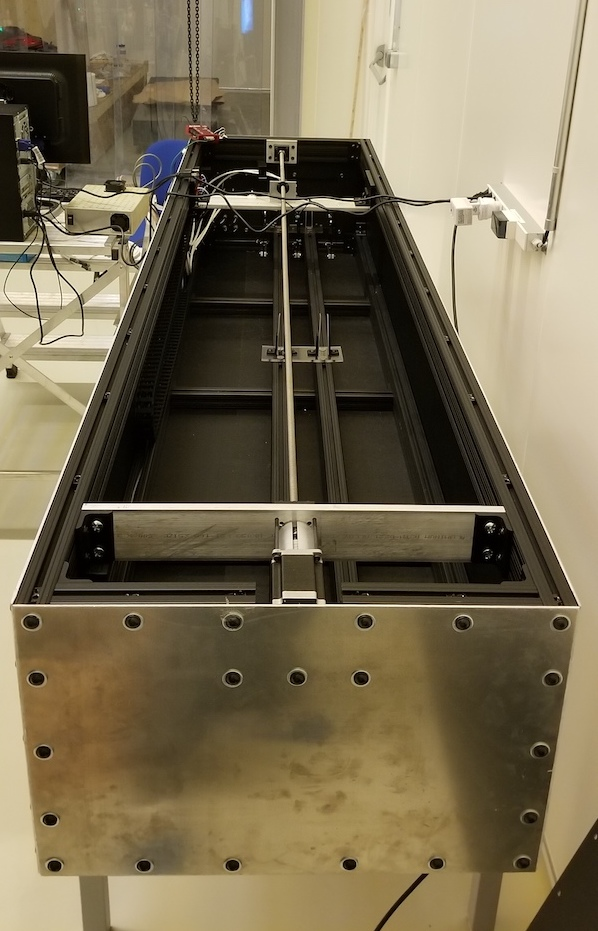
\includegraphics[height=.40\textheight, angle=0]{pds-scanner}
\end{dunefigure}

Access to the \dwords{pd} inside the \dword{apa}s is severely limited once the \dword{ce} cable conduit is in place, so identifying problems early in the process is necessary to minimize schedule issues caused by required \dword{pd} maintenance or repair due to problems detected during installation.

Following the optical scan, the \dword{pd} modules are inserted into an  \dword{apa} at the photon integration area in the cleanroom. The connection to the cable harness, which is pre-installed in the \dword{apa} before wire wrapping, is automatic. An electrical continuity check follows insertion to verify  continuity between the \dword{pd} module and the \dword{pd} cable end connector at the end of the \dword{apa}.

\begin{comment}
Once integrated \dword{apa}s are received in the \dword{sas} for the cleanroom in front of the cryostat, an electrical connectivity test between the cable end exiting the \dword{apa} to be installed and each of the \dword{pd} modules in that \dword{apa} will be performed.  Discussions are underway with the \dword{apa} consortium to determine if the transport frames for shipping the integrated \dword{apa} pairs can be made sufficiently light-tight to allow biasing the photosensors and checking that they are operating properly.  Accessing the \dword{pd} modules involves removing the \dword{ce} cable conduits from the \dword{apa} side tubes, so this is the last time in the installation process that \dwords{pd} can be reached for repair or replacement.  Any repairs to the \dword{pd} system discovered later in the installation process would require returning the \dword{apa} module to this point in the installation sequence.
\end{comment}

As the upper and lower \dword{apa}s are joined on the assembly tower, photon detector cables from the upper to the lower \dword{apa} will be connected, and at that time, continuity checks will be made.

Once the upper and lower \dword{apa}s are joined, the assembled unit will be moved into a coldbox in front of the cryostat for final testing.  This is an opportunity to make a final low-temperature check of the complete \dword{pd} \dword{ce} and cabling chain before installation into the cryostat.  \dword{pd} \dword{fe} electronics boards will be used to read out the photon system during the cold test, and results will be compared to previous \dword{qa} test results.

The \dword{apa} stack is rolled into position in the cryostat following the coldbox test, and the \dword{pd} and \dword{ce} cables connected to the cryostat flange.  At this point, a final continuity check is made from the flange bulkhead to the \dword{pd} module.

Discussions are underway with the installation team to arrange for a one-shift dark test of the installed photon detectors in the cryostat following final installation, verifying end-to-end system operation.

\subsubsection{Calibration system testing}
The laser system is aligned and tested as the lasers are installed. This requires and initial alignment with the alignment laser then testing with the UV laser under controlled conditions. Details of the testing procedures have not yet been developed. The pulsed neutron source will be calibrated offline to verify the shielding design and neutron flux. {\it In situ} the source will be operated in test mode to verify the functionality. 

\begin{comment}
%%%%%%%%%%%%%%%%%%%%%%%%%%%%
\subsection{Environmental, Safety, and Health (ES\&H)}
\label{sec:fdsp-tc-inst-safety}

Fermilab, \fixme{SURF and?}  and \dword{dune} are committed to supporting the health and safety of staff, the community, and the environment in research and operations, as stated in the \dword{lbnf}/\dword{dune} Integrated Safety Management Plan\cite{bib:docdb291}. The safety and health program complies with applicable standards and local, state, and federal legal requirements through Fermilab's Work Smart Set of Standards \fixme{ref -ask Mike A} and the contract between \dword{fra} and the \dword{doe}. \dword{fnal} and the \dword{sdsd} have the host laboratory responsibilities for \dword{lbnf} and \dword{dune} operations at \dword{surf} in Lead, South Dakota.
The Fermilab facilities are further subject to the requirements of the \dword{doe} Workers Safety and Health Program 10 CFR 851\cite{doe-10cfr851}. These requirements are promulgated through the Fermilab Directors Policy Manual, and the \dword{feshm}, which align with the \dword{surf} \dword{esh} manual.

%While \dword{esh} will be  a host laboratory (Fermilab/SDSD) responsibility, a  Global Safety Coordination group will evaluate applicable codes and standards including international code equivalency for the design, assembly, and installation of the \dword{dune} detectors. The Global Safety Coordination group is  a team of engineering and \dword{esh} experts from within \dword{lbnf} and \dword{dune} organizations.  These requirements will be adopted by \dword{dune}, JPO (Joint Project Office), and \dword{lbnf} organizations and used to develop manufacturing, assembly, and installation processes and procedures. 
While \dword{esh} is  a host laboratory (\dword{fnal}'s \dword{sdsd}) responsibility, a  \dword{gsc} will evaluate applicable codes and standards including international code equivalency for the design, assembly, and installation of the \dword{dune} \dwords{detmodule}. The \dword{gsc} is  a team of engineering and \dword{esh} experts from within \dword{lbnf} and \dword{dune} organizations.  These requirements will be adopted by \dword{dune}, \dword{jpo}, and \dword{lbnf} organizations and used to develop manufacturing, assembly, and installation processes and procedures. 
\dword{dune} will develop an %Installation 
\dword{esh} plan for installation that will define %a specific set of 
the \dword{esh} requirements and responsibilities that personnel will be required to follow while  assembling, installing, and constructing equipment at \dword{surf}. % and \dword{itf}. 

{\bf Work Planning and Controls:} The goal of the work planning and \dword{ha} process is to initiate thought about the hazards associated with work activities and how the work can be performed safely. Careful planning of a job assures that it is performed efficiently and safely. Work planning ensures the scope of the job is understood, appropriate materials and tools are available, all hazards have been identified, mitigation efforts established, and all affected employees understand what is expected of them. %\dword{ha} is a critical part of work planning.  
The Work Planning and Hazard Analysis program is documented in Chapters 2060 in the \dword{feshm}.

The shift supervisor will lead %daily 
work planning meetings at the start of each shift to coordinate work activities, review hazards and mitigations, and answer any questions.

{\bf Documentation Approval Process:} The engineering review and approval process of all required documentation includes structural calculations, assembly drawings, load tests, \dwords{ha}, and procedural documents for \fixme{a set of identified?} typical individual tasks.  For the larger operations and systems like \dword{tpc} component factories, the \dword{dss}, cleanroom, and assembly infrastructure, this will be followed by an \dword{orr} by a joint safety committee that visits the site  after reviewing the documentation, and watches the full operation before signing off on the documentation.

{\bf \dword{esh} Support:} Safety starts from the ground up, both on the surface and in the underground facilities. All employees have work stop authority in support of  a safe working environment. Personnel will need to use the necessary \dword{ppe} identified through the \dword{ha} process for the task. A local \dword{esh} coordinator under the direction of the \dword{dune} \dword{esh} Manager will provide daily support for the facilities and attend the %daily 
\fixme{they are either daily or per shift - sounds like `per shift' is correct}
work planning meetings to notify each shift of potential safety issues and constraints, to ensure that  employees have the necessary \dword{esh} training, and to be responsible \fixme{to make sure the workers are responsible? or so that  the coordinator has what they need so that they can be responsible?} for managing \dword{esh} related  documentation including training records, weekly safety reports, near miss and accident reports, and equipment inspection.

{\bf Work Underground} \dword{sdsta} will maintain:
\begin{itemize}
    \item Site Access Control Program through \dwords{tap};
    \item \dword{em} program, which includes an Emergency Response incident command system and an \dword{ert}.  Typically, a small number of employees underground (guides) are also training as first responders to help in a medical emergency.
    
\end{itemize}

{\bf Equipment operation:} All overhead cranes, gantry cranes, fork lifts, motorized equipment trains/carts will be operated only by trained licensed operators. 
Other equipment, e.g., scissor lifts, pallet jacks, hand tools, and shop equipment, may only be operated by people trained
and certified for the particular piece of equipment.

{\bf House cleaning:} All workers underground are responsible for keeping a clean organized work area. Flammable items must be in proper storage cabinets, and items like empty shipping crates and boxes must be removed and %shipped 
transported back to the surface to make space.

{\bf \dword{ppe}:} 
\dword{ppe} is the responsibility of the host laboratory,  %(Fermilab/SDSD) and will be supplied 
which will supply it to all workers. 

{\bf Access and training:}  All \dword{dune} workers requiring access to the \dword{surf} site must (1) register through the \dword{fnal} Users Office to receive the necessary user training and a \dword{fnal} ID number, and they must apply for a \dword{surf} identification badge. % for \dword{dune} activities. 
All \dword{dune} workers will be required to complete \dword{surf} Surface and Underground Orientation classes. Workers accessing the underground must also complete 4850 and 4910 level specific unescorted access training. %A guide must be stationed on all working levels and have received the necessary guide training. 
A properly trained guide will be stationed on all working levels. 

{\bf Requirements at collaborating %laboratories and 
institutions:} All work performed at collaborating institutions will be completed in accordance with the %collaborating 
institution's \dword{esh} policies and programs. 
Equipment and operating procedures provided by the %collaborating 
institution must conform to the \dword{dune} Project \dword{ieshp}. %\dword{esh} and Integrated Safety Management policies and procedures. 
The %collaborating 
institution's \dword{esh} department is responsible for providing \dword{esh}  oversight for all work activities carried out in their facilities. % in collaborating institution facilities. 
\dword{lbnf} and \dword{dune} personnel will also follow the \dword{esh} manual and procedures of the collaborating institutions.

\end{comment}


%DAVID added cryo cold box??%%
%%{Cold Boxes Cryogenics}
\label{sec:fdsp-tc-cryocoldbox}


The  \coldbox{}es will be used to test the \dword{apa}s underground prior to installation.  
The cryogenics supporting the \coldbox{}es  must ensure their reliable and safe operation; to that end, it must
\begin{itemize}
\setlength\itemsep{1mm}
\setlength{\parsep}{1mm}
\setlength{\itemsep}{-5mm}
\item support three \coldbox{}es operating in parallel: %for testing dual \dword{apa}s: 
one in \cooldown mode, two either in steady-state or warm-up modes.
\item allow personnel in the cleanroom during all phases of the purge, \cooldown, operation, and warm-up modes. 
\item test the detector modules at near \dword{lar} temperature.
\item operate 24 hours a day, seven days a week for 10 years.
\item allow remote operations.
\item be located in the vicinity of the \dword{tco}. Space is available on top of the cryogenic mezzanine on the roof of the cryostat.
\end{itemize}

It must operate in the following modes: %fulfill the following modes of operations:

\begin{itemize}
\setlength\itemsep{1mm}
\setlength{\parsep}{1mm}
\setlength{\itemsep}{-5mm}
\item \textbf{purge}: During this mode, air is removed from the system (\coldbox and cryogenic system) and replaced with dry nitrogen. The concentration of moisture is monitored, and when it no longer decreases, the \cooldown can commence.
\item \textbf{\cooldown}: Cold nitrogen is introduced into the system to cool the inside of the \coldbox and the \dword{apa} inside it. %it down and to cool down the detector contained inside the coldbox. 
This should take 24 hours, during which time the temperature decreases from room temperature to about \SI{90}{K}. 
\item \textbf{steady-state operations}: After reaching %the nominal temperature of 
approximately \SI{90}{K}, %the value is maintained for 48 hours, during which 
the detector is turned on and fully tested. % at cold. 
This takes about 48 hours.
\item \textbf{warm-up}: After completing the test, the system is %slowly 
warmed up to room temperature over a period of 24 hours. %This should take 24 hours, during which the temperature goes from approximately \SI{90}{K} to room temperature.
\end{itemize}

\begin{dunetable}
[\Coldbox  cryogenics system parameters] %for specifications]
{lc}
{tab:table-cryo-coldboxes}
{Table of parameters for the \coldbox cryogenics system.}
Parameter & Value 
\\ \toprowrule
Dual \dword{apa} thermal mass &  1,600 kg\\ \colhline
Temperature uniformity & $+60$ K / $-0$ K \\ \colhline
Electronics load & 300 W \\ \colhline
\Coldbox insulation thickness &  0.3 m \\ \colhline
Target \cooldown temperature &  \SI{90}{K} \\ \colhline
Target \cooldown duration &  24 hr \\ \colhline
Target steady-state duration &  48 hr \\ \colhline
Target warm-up duration &  24 hr \\ \colhline
Maximum cooling power  &  \SI{13}{kW}  \\ \colhline 
Maximum liquid nitrogen consumption  &  \SI{300}{l/hr}  \\ \colhline 
\end{dunetable}

The evaporation of liquid nitrogen provides the cooling power for the system. Warm nitrogen and a heater provide the heating power. At peak consumption, the expected maximum heat load is \SI{8.5}{kW}. Assuming a 50\% margin on the refrigeration load, the cryogenics system requires \SI{13}{kW} of net cooling power at peak consumption, which equals about \SI{300}{l/hr} of evaporating liquid nitrogen.

Two layouts are currently under consideration: (1) a closed loop with mechanical refrigeration, in which liquid nitrogen is generated {\it in situ}, circulated, and the spent nitrogen recondensed before being put back into the system; and (2) open loop, in which liquid nitrogen is transported underground by means of portable dewars, circulated, and the spent nitrogen vented away. For the closed loop, we would need a mechanical refrigeration capable of supplying \SI{13}{kW} of cooling. For the open loop, it is possible to use a \SI{2000}{l} dewar, which is commercially available and transportable up and down the Ross Shaft inside the cage. To supply the required amount of nitrogen, four trips per day are needed.

The current versions of the closed loop and open loop systems are presented in Figures~\ref{fig:mechanical-refrigeration} and~\ref{fig:LN2}, respectively. 

\begin{dunefigure}[\Coldbox cryogenics support system based on mechanical refrigeration ]{fig:mechanical-refrigeration}
  {Layout of the cryogenics supporting the \dword{apa} test facility with mechanical refrigeration (closed loop).}
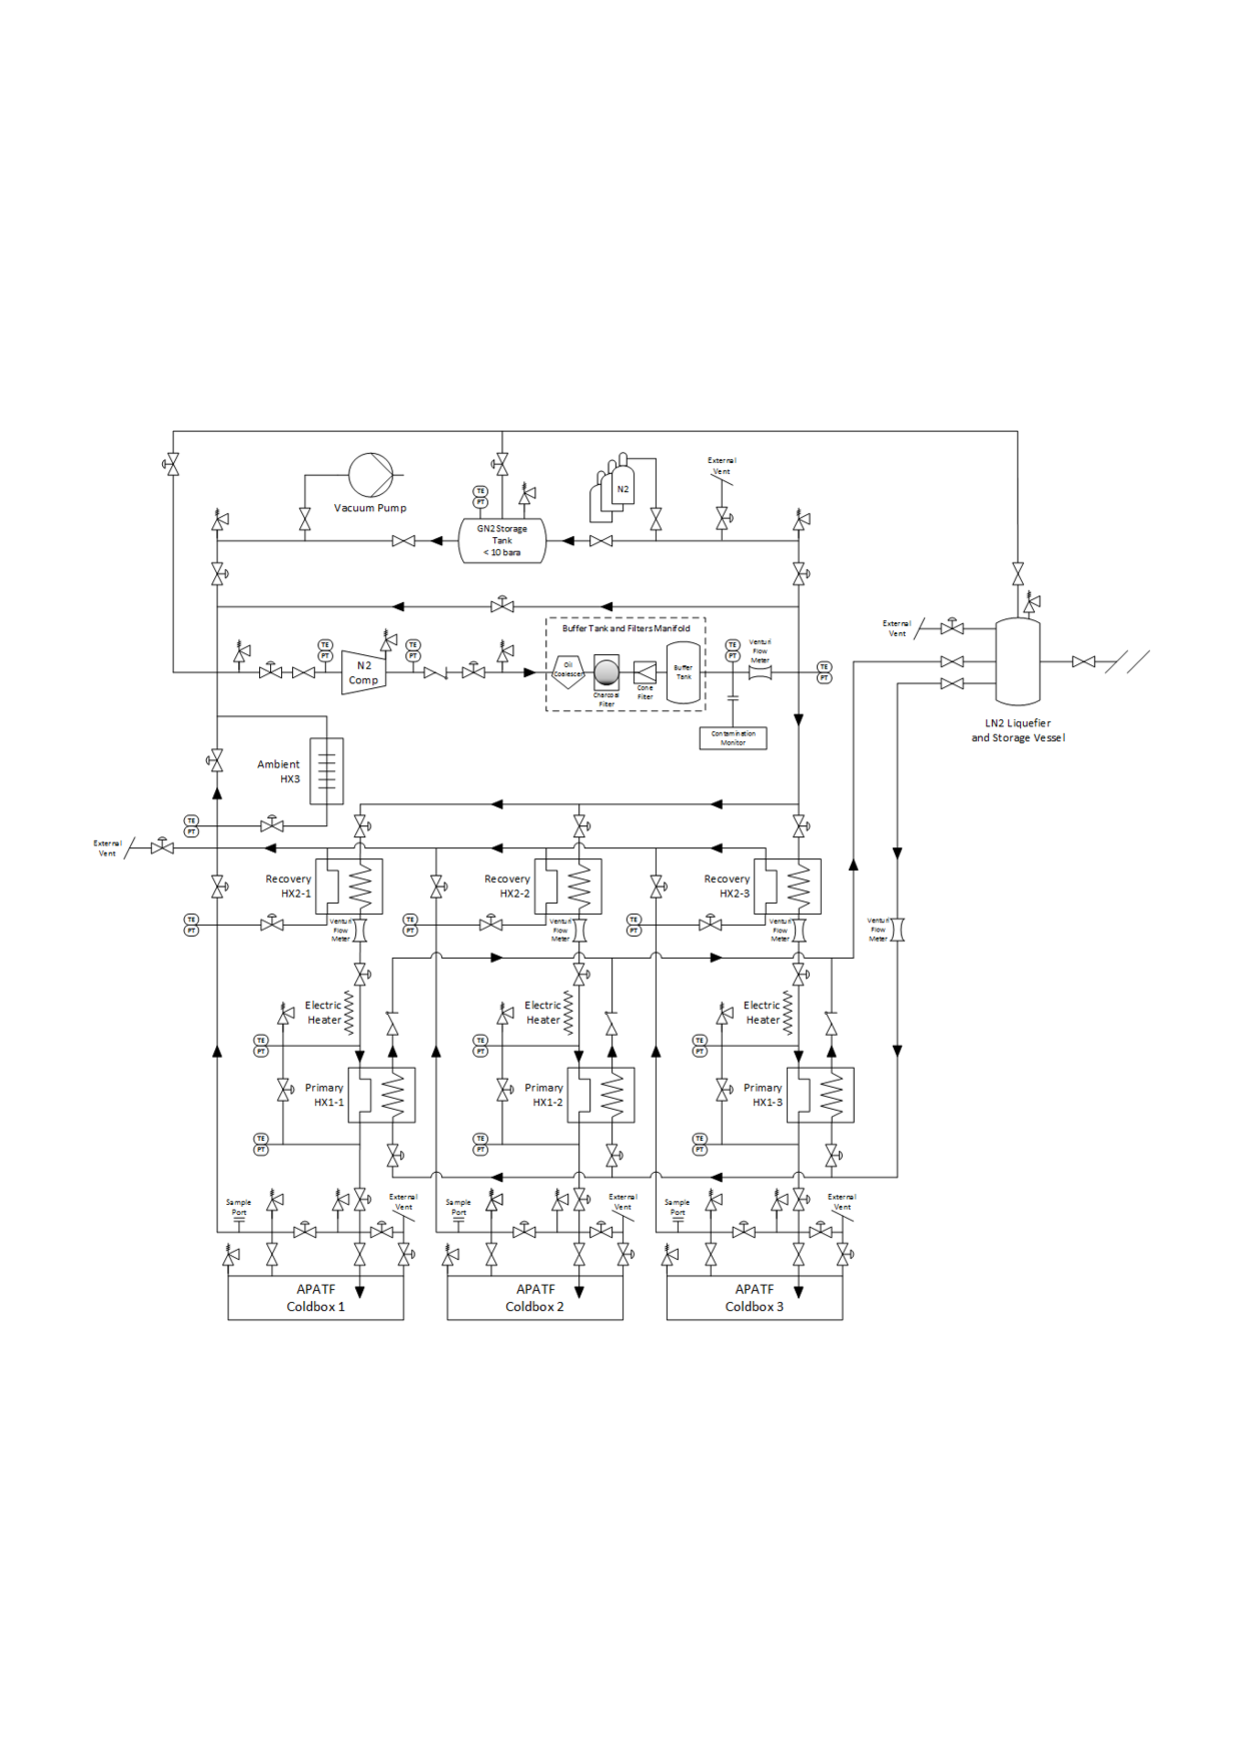
\includegraphics[width=.98\textwidth]{graphics/Cryo-cold-box-mechanical.pdf}
\end{dunefigure}

\begin{dunefigure}[\Coldbox cryogenics support system based on LN2 ]{fig:LN2}
  {Layout of the cryogenics supporting the \dword{apa} test facility with open loop refrigeration (open loop).}
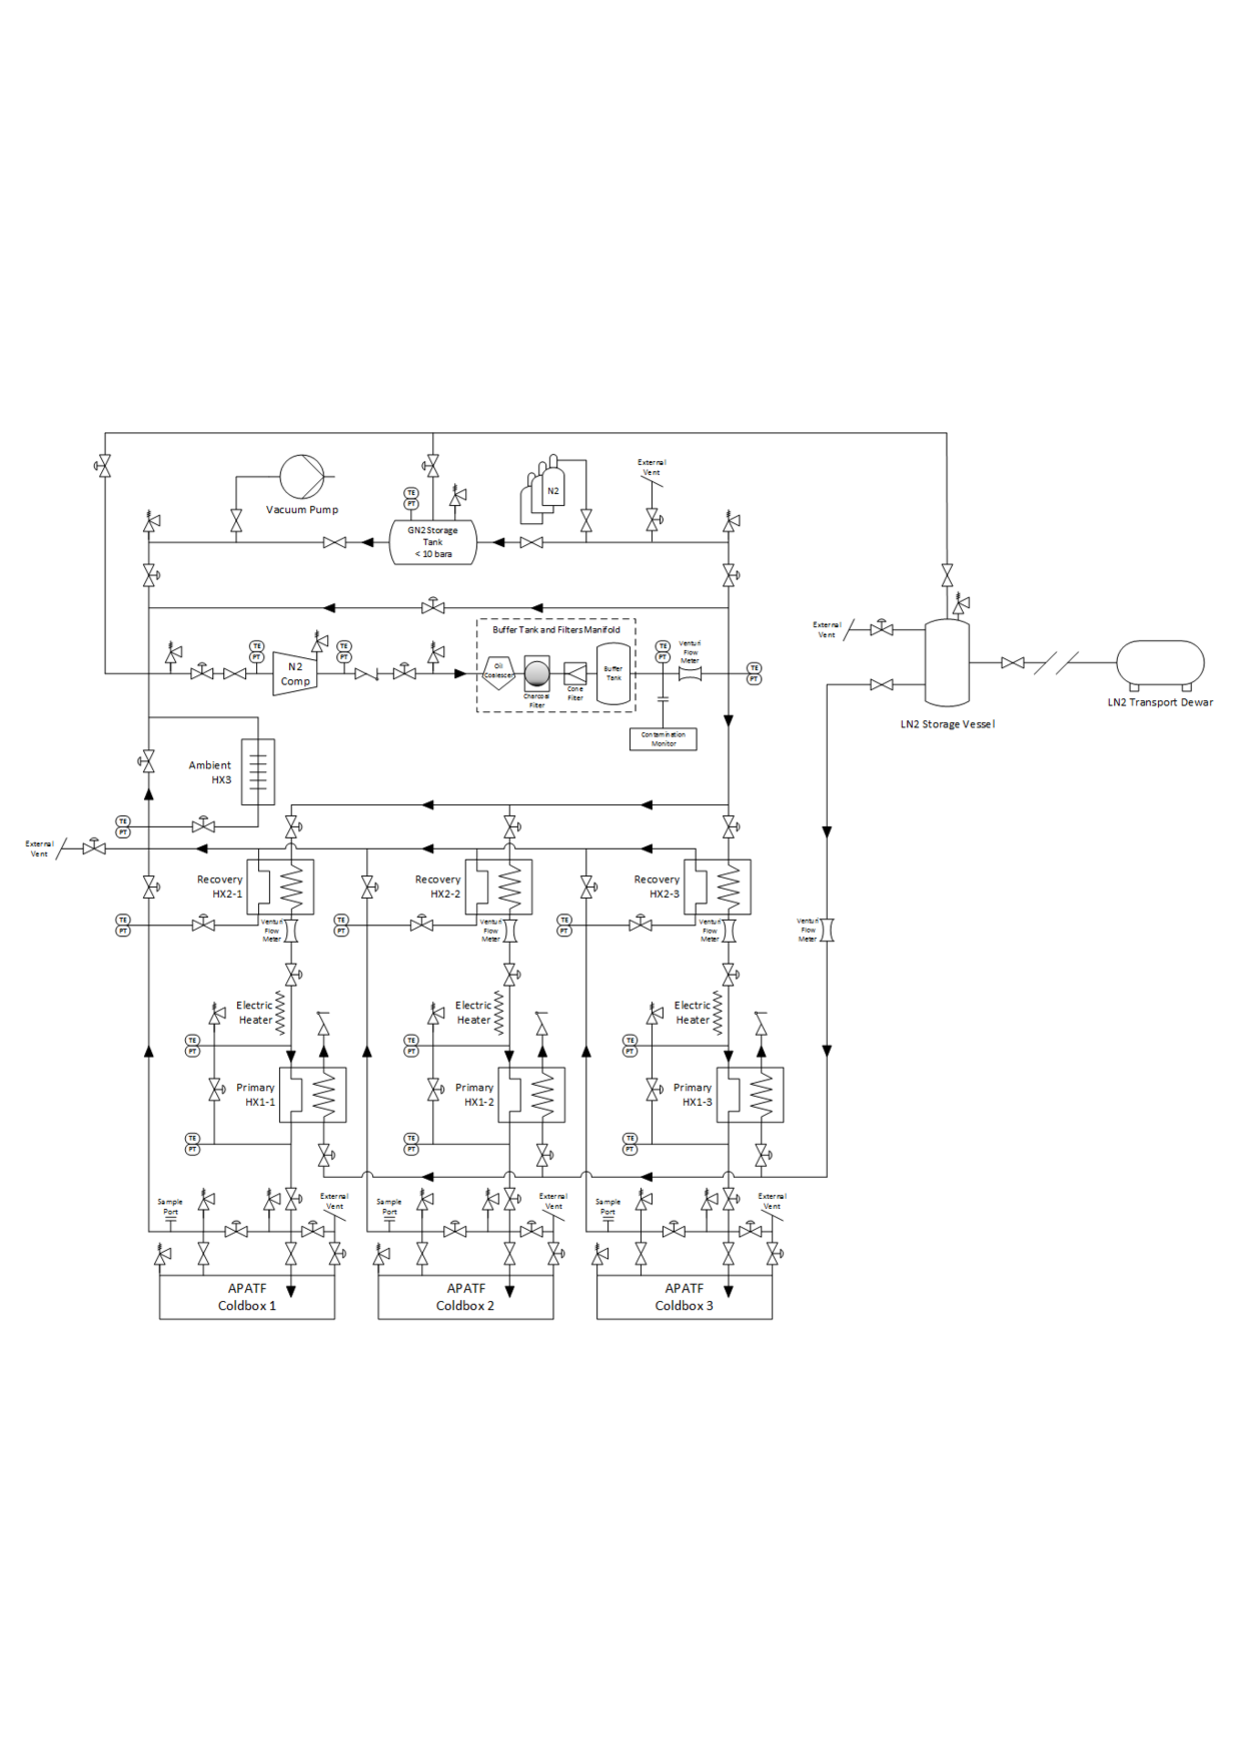
\includegraphics[width=.98\textwidth]{graphics/Cryo-cold-box-LN2.pdf}
\end{dunefigure}



%%%%%%%%%

\section{Cost and Schedule}



%%%%%%%%%%%%%%%
\subsection{Costs}

The costs for the \dword{jpo} are still being compiled. These costs will first be presented to the DOE in the second half of August of 2019. After the data is submitted to the DOE the table in the \dword{tdr} will be updated.



\begin{dunetable}
[Cost Summary]
{p{0.5\textwidth}p{0.2\textwidth}p{0.2\textwidth}}
{tab:XXcostsumm}
{Cost Summary}   
Cost Item & M\&S (k\$ US) & Labor Hours \\ \toprowrule
\rowcolor{dunepeach} Design, Engineering and R\&D &  &     \\ \colhline
 (E.g., Photosensors design) &     &             \\ \colhline
 (E.g., Mechanics design) &     &             \\ \colhline
 &     &             \\ \colhline
 &     &             \\ \colhline
 &     &             \\ \colhline
 &     &             \\ \colhline
\rowcolor{dunepeach} Production Setup &  &     \\ \colhline
 (E.g., Photosensors production setup)  &     &             \\ \colhline
 &     &             \\ \colhline 
 &     &             \\ \colhline
 &     &             \\ \colhline 
 &     &             \\ \colhline
 &     &             \\ \colhline
\rowcolor{dunepeach} Production &  &     \\ \colhline
 (E.g., Photosensors production)  &     &             \\ \colhline
 &     &             \\ \colhline 
 &     &             \\ \colhline
 &     &             \\ \colhline 
 &     &             \\ \colhline
 &     &             \\ \colhline
\rowcolor{dunepeach} DUNE FD Integration \& Installation  &  &     \\ \colhline
 &     &             \\ \colhline
 &     &             \\ \colhline 
 &     &             \\ \colhline
 &     &             \\ \colhline 
 &     &             \\ \colhline
 (last line) &     &             \\
\end{dunetable}

%force the figure to appear here before the next section.
\clearpage

\subsection{Schedule}

The detector installation planning hinges on the date when the \dword{jpo} is permitted to begin work underground. According to the \dword{dune} \dword{cf} schedule the \dword{jpo} receives the \dword{aup} for  the north cavern and \dword{cuc} in \cucbenocc{}.  The  \dword{sdwf} will be in place approximately 6 months before the warm structure installation begins, i.e., in spring 2022. Building the schedule for the \dword{spmod} 1 Installation after \dword{aup} is a complicated dance that depends on many entities including \dword{cf}, \dword{lbnf}, and \dword{sdsta}.  The maximum number of people allowed underground is 144 which is the number of people that can be evacuated in one hour.  This places a hard bound on how much work can be perfored underground at any time and is particularly critical during the excavation of Cavern 3 when \dword{cf} is still active. Figure \ref{fig:Overview-of-SinglePhase-Schedule} shows the main activities for the \dword{detmodule} \#1 installation and  the high level milestones are shown in Table \ref{tab:sp-iic-sched}.

The cost, schedule, and labor estimates are based on two 10 hour shifts per day, 4 days a week. Work efficiency should be a maximum of 70 percent.  The cage ride, and shift meetings, lunch, coffee breaks, and gowning to go into the cleanroom takes up approximately 2-3 hours per day. Some low level of effort is planned on Friday, Saturday, and Sunday to monitor the \coldbox{}es and take data. 




%This is a standard table template for the TDR schedules.  It contains overall FD dates from Eric James as of March 2019 (orange) that are held in macros in the common/defs.tex file so that the TDR team can change them if needed. Please do not edit these lines! Please add your milestone dates to fit in with the overall FD schedule. 

\begin{dunetable}
[\dword{sp} Installation, Integration, and Commissioning Milestones]
{p{0.65\textwidth}p{0.25\textwidth}}
{tab:sp-iic-sched}
{\dword{sp} Installation, Integration, and Commissioning Schedule}   
Milestone & Date (Month YYYY)   \\ \toprowrule
Ash River phase 0 complete &      \\ \colhline
Foreman/Lead Mechanical engineer starts& \\ \colhline
Ash River phase 1 complete &      \\ \colhline
Installation Preliminary Design Review &      \\ \colhline
Ash River phase 2 complete &      \\ \colhline
Installation Final Design Review  &      \\ \colhline
\rowcolor{dunepeach} Start of \dword{pdsp}-II installation& \startpduneiispinstall      \\ \colhline
\rowcolor{dunepeach} Start of \dword{pddp}-II installation& \startpduneiidpinstall      \\ \colhline
 \dword{cuc} \dword{prr} &      \\ \colhline
Installation \dword{prr} &      \\ \colhline
\rowcolor{dunepeach}South Dakota Logistics Warehouse available& \sdlwavailable      \\ \colhline
Begin procurement of \dword{cuc} equipment  &   April 2022   \\ \colhline
Start production of installation infrastructure Detector \#1 & August 2022     \\ \colhline
\rowcolor{dunepeach}Beneficial occupancy of cavern 1 and \dword{cuc}& \cucbenocc      \\ \colhline
Start construction warm structure cryostat \#1   & October 2022     \\ \colhline
Start outfitting of \dword{cuc}  &  October 2022    \\ \colhline
\rowcolor{dunepeach} \dword{cuc} counting room accessible& \accesscuccountrm      \\ \colhline
Start installation of  cold structure Cryostat\#1 &  August 2023    \\ \colhline
Start installing Detector\#1 infrastructure  &  August 2023    \\ \colhline
\rowcolor{dunepeach}Top of \dword{detmodule} \#1 cryostat accessible& \accesstopfirstcryo      \\ \colhline
Begin Detector\#1 installation   &   June 2024   \\ \colhline

\rowcolor{dunepeach}Start of \dword{detmodule} \#1 TPC installation& \startfirsttpcinstall      \\ \colhline
\rowcolor{dunepeach}End of \dword{detmodule} \#1 TPC installation& \firsttpcinstallend      \\ \colhline
TCO detector \#1 closed  &  July 2025    \\ \colhline
\rowcolor{dunepeach}Top of \dword{detmodule} \#2 accessible& \accesstopsecondcryo      \\ \colhline
Start of cryogenic operation for detector \#1  &  August 2025    \\ \colhline
 \rowcolor{dunepeach}Start of \dword{detmodule} \#2 TPC installation& \startsecondtpcinstall      \\ \colhline
\rowcolor{dunepeach}End of \dword{detmodule} \#2 TPC installation& \secondtpcinstallend      \\ \colhline
Start of  detector\#1 commissioning  & January 2027     \\ \colhline                        \\
\end{dunetable}



\begin{dunefigure}[Overview of the single-phase schedule]
{fig:Overview-of-SinglePhase-Schedule}
{Schedule Overview of the Single Phase Detector \#1}                
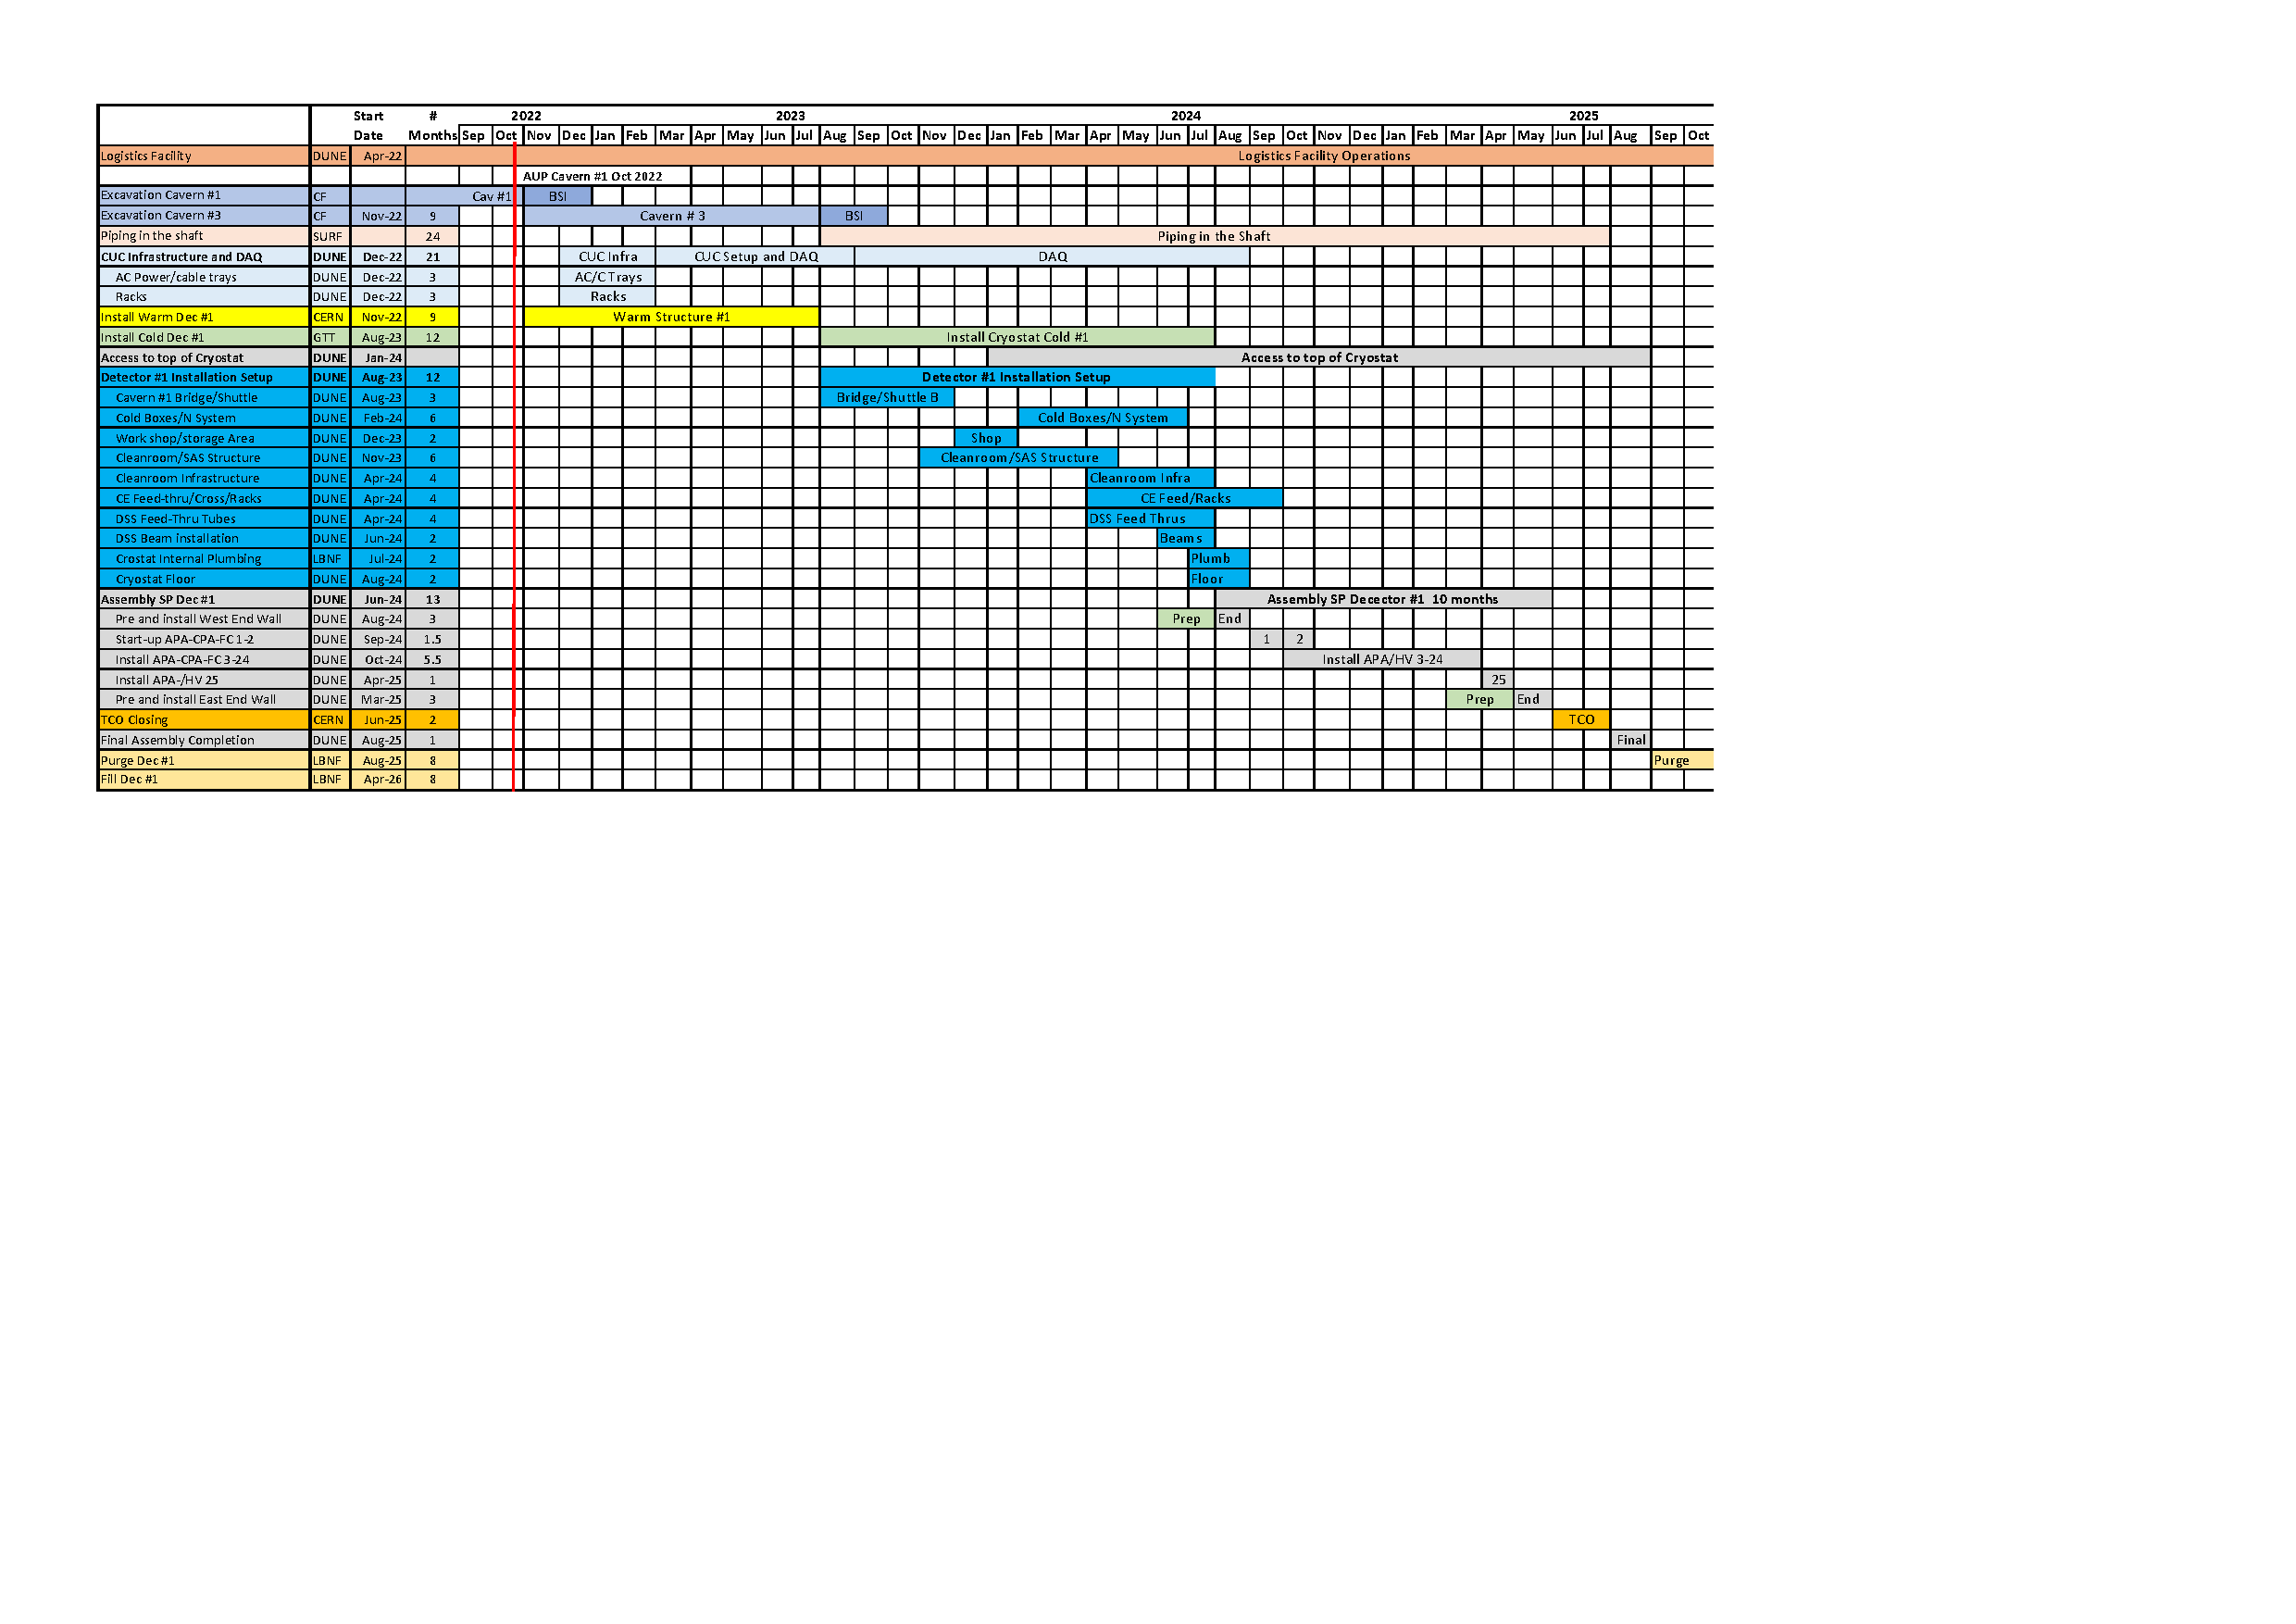
\includegraphics[width=0.98\textwidth]
{Overview-of-SinglePhase-Schedule}
\end{dunefigure}



As described earlier there are three basic schedule phases for Detector 1 installation:

\begin{itemize}
    \item {\bf \dword{cuc} Installation Phase:}
    This period, which is described in detail in section \ref{sec:fdsp-tc-inst-CUC}, can start once \dword{aup} has been received for the north cavern and the \dword{cuc}. This is also the same time that excavation of the south cavern and installation of the warm structure by \dword{lbnf} begins. As no more than 144 \dwords{fte} will be allowed underground at a time,  access to the underground area will be minimal during this period for \dword{dune} personnel.  Work in this period is limited to work inside the \dword{cuc} and surface dataroom. Installing the basic rack infrastructure in the datarooms will take an estimated three months, and then installation and testing of the \dword{daq} will continue over the next 12 month period. The \dword{daq} is needed at the start of detector installation.  
    
    \item {\bf Installation Setup Phase:} This phase,  described in detail in section \ref{sec:fdsp-tc-inst-setup}, is when the majority of the infrastructure is installed. 
    This is a critical training period, so getting lead-workers, riggers, and equipment operators familiar with the tasks is a priority, and adjusting crews to ensure balanced teams.  
    Before this phase, the \dword{dune} trial assembly equipment at Ash River will be used to begin the training process. This is a more difficult phase to schedule and may require frequent adjustment, with multiple projects going forward at once.
    Immediately after the cryostat warm structure is complete the north-south bridge is constructed. Following this the bridge crane under the bridge can be installed. A few months after the cryostat warm structure is complete the \dword{cf} work is also complete and the 80 of 144 underground workers which \dword{cf} had been using are available to the \dword{jpo}, working two 10 hour shifts per day begins, and the \dword{uit} team doubles in size.  Peripheral work on the cleanroom structure and assembly towers can then begin as they will not take up too much floor space. Once the  cryostat cold structure is approximately six months into the installation schedule most of the foam has been installed and floor space becomes available in the north cavern. The \coldbox construction must begin immediately at this point because the welding takes approximately six months. In parallel, the machine shop area can be set up. As the membrane installation nears completion the walls of the cleanroom can be installed and the remaining equipment. 
    
    Installation of the \dword{dss} could begin during the final installation stages of the cryostat cold structure because they both require full-height scaffolding for the welding on the top of the cryostat. The \dword{protodune} \dword{dss} was installed this way. This requires a crew on top of the cryostat installing the \dword{dss} support feedhroughs from the top, as shown in Figure~\ref{fig:install-dss-feedthru}.  The details have not yet been worked out with the contractor, so work may be done in stages. 

    
    \item {\bf Detector Installation Phase:} The final detector installation phase begins with an operational readiness review to check that all documentation and procedures are in place. After the east endwalls are installed, a start-up period of 1.5 months begins for the first two rows of \dword{tpc} components.  To meet this schedule, three assembly lines, three coldboxes, and separate crews in the cryostat, all working in parallel are needed.  It will take 5.5 months to install rows 3-24 and about 1 month for row 25. Closing the \dword{tco} will take approximately two months for the cryostat cold structure contractor. During this time, there is no access to the cryostat.  Once this is completed, the final instrumentation is completed, and the purge can begin. 
    
\end{itemize}



  




% clear the figure buffer before starting the next section
%\clearpage


\subsection{Detector Commissioning Phase}
\label{sec:fdsp-tc-inst-comiss}

After the \dword{spmod} is installed in the cryostat, much work remains before it can be operated. 
The cryostat manufacturer must come back to close the \dword{tco}. 
First they install the missing steel panel which completes the cryostat's outer structural hull. 
Then the remaining foam blocks and membrane panels which were stored inside the cryostat are installed. 
In this period personnel access is through the roof's access portholes. 



In parallel, the \lar pumps are installed at the ends of the cryostat and final connections are made to the recirculation plant. Next, everything is leak tested, and the cryogenics plant can be brought into operation. The system first purges the air inside the cryostat  by injecting pure \dword{gar} at the bottom  at a rate that fills the cryostat volume uniformly but faster than the diffusion rate. This ``piston purge'' process produces a column of \dword{gar}  that rises through the volume and pushes out the air.  When the piston purge is complete, misting nozzles inject a liquid-gas mix into the cryostat that cools the detector components at a controlled rate. 


Once the detector is cold, the filling process begins. \dword{lar} stored at the surface  at \dword{surf} is vaporized, brought down the shaft in gaseous form, and re-condensed underground. The \lar then flows through filters to remove any H$_2$O and O$_2$ before entering the cryostat. Given the volume of the cryostat and the limited cooling power for recondensing, \num{12} months will be required to fill the first \dword{detmodule}. The detector readout electronics will be on monitoring the status of the detector. 

Testing and constant monitoring of the detector will take place from \dword{tco} closing until the end of the filling process. 
Before the last access port is sealed:
\begin{enumerate}

    \item A pedestal and \dword{rms} characterization of all cold electronic channels will verify that all \dword{apa} front-end boards are responding and no dead channel or new noise sources arose following the \dword{tco} closing.
    
    \item A noise scan of all \dword{pd} channels is performed as last check before sealing.

    \item Each \dword{apa} wireplane will be checked to verify it is isolated from the \dword{apa} frame and properly connected to its \dword{hv} power supply through the following steps:
    
\begin{itemize}

    \item The \dword{shv} connector of each wireplane bias channel will be unplugged at the power supply, and both the resistance and capacitance between inner conductor and ground will be measured. 
    The resistance should show the wireplane is electrically isolated from the ground, while the capacitance value should match that of the cold \dword{hv} cable and the capacitance of the circuit on the \dword{apa} top frame.

    \item \SI{50}{V} is applied to each wireplane and the current drawn checked against the expected value.
    
    \item Nominal voltages are applied to each wireplane, and the current drawn is checked against the expected value. 
    
\end{itemize}

    \item A low \dword{hv} (i.e., \SIrange{1}{2}{kV}) is applied to the cathode, and the current drawn is checked against the expected value to ensure the integrity of the \dword{hv} line.

\end{enumerate}

During the piston purge process periodic monitoring of \dword{apa}, \dword{ce}, and \dword{pd} system noise (pedestal, \dword{rms}) will occur.

A number of the following tests, in addition to new ones, will instead take place during the cool-down phase:

\begin{enumerate}


    \item Each \dword{apa} wireplane isolation and proper connection to its \dword{hv} power supply will be checked at regular time intervals as was done before sealing the cryostat.
    
    \item \SIrange{1}{2}{kV} will be held on the cathode, and the current drawn will be  monitored constantly to observe the trend in temperature of the total resistance.
    
    \item \dword{ce} noise figures (pedestal, \dword{rms}) will be measured at regular intervals and their trends with temperature recorded.
    
    \item \dword{pd} system noise (pedestal, \dword{rms}) will be measured at regular intervals and its trend with temperature recorded.
    
     \item Values of the temperature sensors deployed in several parts of the cryostat will be monitored constantly to watch the progress of the cool down phase and to relate the temperature to the behavior of the other \dword{spmod} subsystems. 
     
\end{enumerate}

Regular monitoring of \dword{ce} and \dword{pd} noise, as well as checks of wireplane isolation and proper connections to the bias supply system will continue throughout the filling, recording noise variations as a function of the progressively reduced temperature. In addition,

\begin{enumerate}

    \item As each purity monitor is submerged in liquid, it will be turned on every eight hours to control \dword{lar} purity.
    
    \item As soon as top ground planes are submerged, \dword{hv} on the cathode will be raised up to \SI{10}{V} to check that the current drawn by the system agrees with expectations.

\end{enumerate}

Once the \dword{detmodule} is full, the drift \dword{hv} will be carefully ramped up following these steps:

\begin{enumerate}

    \item The need for a filter regeneration is evaluated before starting any operation;

    \item Once filter regeneration is completed (if needed), the \dword{lar} surface is examined using cameras to verify that the surface is flat, with no bubbles or turbulence;
    
    \item \dword{lar} recirculation is started, and \dword{lar} surface is examined again to see if activating the recirculation system introduced any turbulence into the liquid;
    
    \item Wait one day after beginning  recirculation to stabilize the \dword{lar} flow inside the \dword{detmodule}, then start the \dword{hv} ramp up.
    
\end{enumerate}

Cathode voltage is raised in steps over three days. 
On the first day, cathode voltage is first raised to \SI{60}{kV}, then to \SI{90}{kV} after waiting two hours, and finally to \SI{120}{kV} after waiting another two hours, and then left at this value overnight.
On the second day, cathode voltage is first raised to \SI{140}{kV}, then to \SI{160}{kV} after waiting four hours, and then left at this value overnight. 
On the third day, cathode voltage is first raised to \SI{170}{kV} and then to the nominal operating voltage of \SI{180}{kV} after waiting four hours. 
During each \dword{hv} ramp up, all \dword{ce} current draws are monitored, and the procedure is stopped if any of the current draws go out of the allowed range. 
During each waiting period, regular \dword{daq} runs monitor \dword{ce} and \dword{pd} noise and response, while cathode \dword{hv} and current draw stability are constantly monitored.

In \dword{pdsp}, this process took three days, after which the system was  ready for data-taking. With a detector twenty times larger, the process will take longer, but the turn on time should still be relatively short. 



\section{Environmental, Safety, and Health (ES\&H)}
\label{sec:fdsp-tc-safety}

 Volume \volnumbertc{}, Section~\ref{vl:tc-ESH} of the \dword{dune} \dword{tdr} outlines the requirements and regulations that \dword{dune} work must comply with, whether (1) at \dword{fnal}, (2) in areas  leased by \dword{fnal} or the \dword{doe}, (3) in unleased space at \dword{surf}, or (4) at collaborating institutions.
 
%%%%%%%%%%%%%%%%%%%%%%%%%%%%%%%%%
\subsection{Documentation Approval Process}


\dword{dune} implements an engineering review and approval process for all required documentation, including structural calculations, assembly drawings, load tests, \dwords{ha}, and procedural documents for a comprehensive set of identified individual tasks.  For the larger operations and systems like \dword{tpc} component factories, the \dword{dss}, cleanroom, and assembly infrastructure, a joint safety committee also reviews the documentation then visits the site to conduct
 an \dword{orr}. Before signing off on the documentation for an operation, the committee watches it being performed. 
 
 Structural calculations, assembly drawings and proper documentation of  load tests, hazard analyses, and procedures for various items and activities will require review and approval before operational readiness is granted. 

 
%%%%%%%%%%%%%%%%%%%%%%%%%%%%%%%%%
\subsection{Support and Responsibilities}

An \dword{esh} coordinator, who will report to the \dword{dune} Project \dword{esh} manager, has overall \dword{esh} oversight responsibility for the \dword{dune} activities at the  \dword{sdwf} and on the \dword{surf} site. 
This person coordinates any \dword{esh} activities and facilitates the resolution of any issues that are subject to the requirements of the \dword{doe} Workers Safety and Health Program, Title 10, Code Federal Regulations (CRF) Part 851 (10 CFR 851) (see Volume~\volnumbertc{}).  The \dword{esh} coordinator facilitates training and runs weekly safety meetings. This person is also responsible for managing \dword{esh}-related  documentation including training records, \dword{ha} documents, weekly safety reports, records on materials-handling equipment, near-miss and accident reports, and equipment inspection.

All employees have work stop authority in support of  a safe working environment. 

%%%%%%%%%%%%%%%%%%%%%%%%%%%%%%%%%
\subsection{Safety Program}

Using the \dword{nova} Far Detector Laboratory as a guideline for remote facilities, several other key documents will guide the \dword{fd} installation safety program, as follows:

\begin{enumerate}
\item	Fire Safety and Building Emergency Evacuation Plan, which includes the fire evacuation plan, fire safety plan, lockdown plans, and the site plan;
\item	\dword{ha} document, which describes all typical hazards and their mediation procedures; 
\item	Safety Data Sheets (SDS), 
\item	Respiratory Plan, as required for chemical or ODH hazards, and 
\item	Training Program, which covers required certifications and  training records.
\end{enumerate}


During the installation setup phase, as new equipment is being installed and tested, new employees and collaborators will be trained, and larger teams from the consortia, \dword{sdsd},  and contractors will need access to the underground facilities.  Given the maximum of 140 \dword{fte} underground at any given time, we will move from one to two shifts per day at this point. 


Unlike most items, the \coldbox and cryogenics system will not be %fully 
tested during the trial assembly work at Ash River. 
While the new \coldbox design is very similar to \dword{pdsp}'s, it will be operated under \dword{doe} and \dword{feshm} regulations.  Procedures for operating the \coldbox will be written according to the established requirements.

\fixme{this next pgraph not needed IMO. anne} During this phase, \dword{lbnf} will be completing the cold structure on \dword{detmodule} \#1 and beginning the warm structure on  \dword{detmodule} \#2. Once \cooldown begins on module \# 1, unlike for \dword{pdsp}, it will be safe for workers to remain in the cleanroom.  

  

\fixme{the next pgraph should be in Steve's volume}

While \dword{esh} is  a host laboratory responsibility, a  \dword{gsc} will evaluate applicable codes and standards, including international code equivalency for the design, assembly, and installation of the \dword{dune} \dwords{detmodule}. The \dword{gsc} is a team of engineering and \dword{esh} experts from within \dword{lbnf} and \dword{dune} organizations.  The \dword{dune}, \dword{jpo}, and \dword{lbnf} organizations will develop manufacturing, assembly, and installation processes and procedures according to the \dword{gsc}'s recommendations. 

\dword{dune} will develop an  \dword{esh} plan for detector  installation that defines  
the \dword{esh} requirements and responsibilities for personnel during  assembly, installation, and construction of equipment at \dword{surf}. It will cover at least the following areas:

{\bf Work Planning and \dword{ha}:} The goal of the work planning and \dword{ha} process is to initiate thought about the hazards associated with work activities and plan how to perform the work. Work planning ensures the scope of the job is understood, appropriate materials and tools are available, all hazards are identified, mitigation efforts are established, and all affected employees understand what is expected of them. 
The Work Planning and Hazard Analysis program is documented in Chapters 2060 in the \dword{feshm}.

The shift supervisor and the \dword{esh} coordinator  will lead a work planning meeting at the start of each shift  to (1) coordinate the work activities, (2) notify the workers of potential safety issues, constraints, and hazard mitigations, (3) ensure that employees have the necessary \dword{esh} training and \dword{ppe}, and (4) answer any questions.

{\bf Access and training:}  All \dword{dune} workers requiring access to the \dword{surf} site must (1) register through the \dword{fnal} Users Office to receive the necessary user training and a \dword{fnal} identification number, and (2) they must apply for a \dword{surf} identification badge. 
The workers will be required to complete \dword{surf} Surface and Underground Orientation classes. Workers accessing the underground must also complete 4850L and 4910L specific unescorted access training, and obtain a \dword{tap} for each trip to the underground area; this is required as part of \dword{surf}'s Site Access Control Program. 
A properly trained guide will be stationed on all working levels. 

{\bf \dword{ppe}:} 
The host laboratory is responsible for supplying appropriate \dword{ppe} to all workers. 

{\bf \dword{em} program} The \dword{sdsta} will maintain an Emergency Response incident command system and an \dword{ert}.  The guides on each underground level will be trained as first responders to help in a medical emergency.
  
  
  {\bf House cleaning:} All workers are responsible for keeping a clean organized work area. This is particularly important underground. Flammable items must be in proper storage cabinets, and items like empty shipping crates and boxes must be removed and 
transported back to the surface to make space.


{\bf Equipment operation:} All overhead cranes, gantry cranes, fork lifts, motorized equipment, e.g., trains and carts, will be operated only by trained  operators. 
Other equipment, e.g., scissor lifts, pallet jacks, hand tools, and shop equipment, will be operated only by people trained
and certified for the particular piece of equipment.


%%%%%%%%%%%%%%%%%%%%%%%%%%%%%%%%%%%%%%%%%%%%%%%%%%%%%%%%%%%%%%%%%%%%
%\section{Integration and Test Facility (ITF)}
%\label{sec:fdsp-tc-itf}

%\section{Integration and Test Facility (ITF)}
\label{sec:fdsp-tc-itf}

%%%%%%%%%%%%%%%%%%%%%%%%%%%%
\subsection{Introduction}
\label{sec:fdsp-tc-itf-intro}

The components of the DUNE detectors will be manufactured in many numerous different countries and locations. For many of the parts it is reasonable to ship the components to the logistics warehouse and then receive the equipment underground where it can be installed. However the  cold electronics and the photon detectors are tightly coupled to the APA. The wires and filters on the APA form part of the electronics circuit and the photon supports and cabling are built into the APA. The work to integrate the CE and PD into the APA is large and the risk of damaging the components is significant so it is planned to integrate the components as early as possible and then thoroughly test the complete assembly. In order to avoid having to create integration testing facilities at each factory one central facility will be established in South Dakota near the SURF site  (within 1 hour drive). In this Integration Test Facility (ITF) the APA, CE and PD modules will arrive, undergo initial tests, be integrated together, undergo a set of warm tests, and then 10\% of the complete assemblies will be cold tested. As the fabrication of the APA assemblies must start 2 years before the completion of the detector installation in order to have enough time to fabricate all the APA the ITF needs to also be operational on the same timescale. The specifications for the ITF are summarized in Table \ref{tab:tcps-itf-spec}.

\begin{dunetable}
[ITF Specifications]
{cc}
{tab:tcps-itf-spec}
{Summary of the high level specifications for the ITF. The building requirements are covered separately in a separate section.}
Parameter & Specification \\ \toprowrule
Cleanroom & The ITF cleanroom shall meet ISO-8 standard per ISO-14644 \\ \colhline
Filtered Lights & <520 nm for long exposure and <400 for exposures less than 2 weeks \\ 
\end{dunetable}

\href{https://lbne2-docdb.fnal.gov/cgi-bin/private/RetrieveFile?docid=8348&filename=UVblockerTests.pdf&version=1 }{UV light filter Study}

%%%%%%%%%%%%%%%%%%%%%%%%%%%%
\subsection{APA-CE-PD integration}
\label{sec:fdsp-tc-itf-integ}
\begin{dunefigure}[ITF Cleanroom Layout]{fig:fdsp-tc-itf-clean}
{Conceptual layout of the cleanroom for the APA-CE-PD integration and testing.}
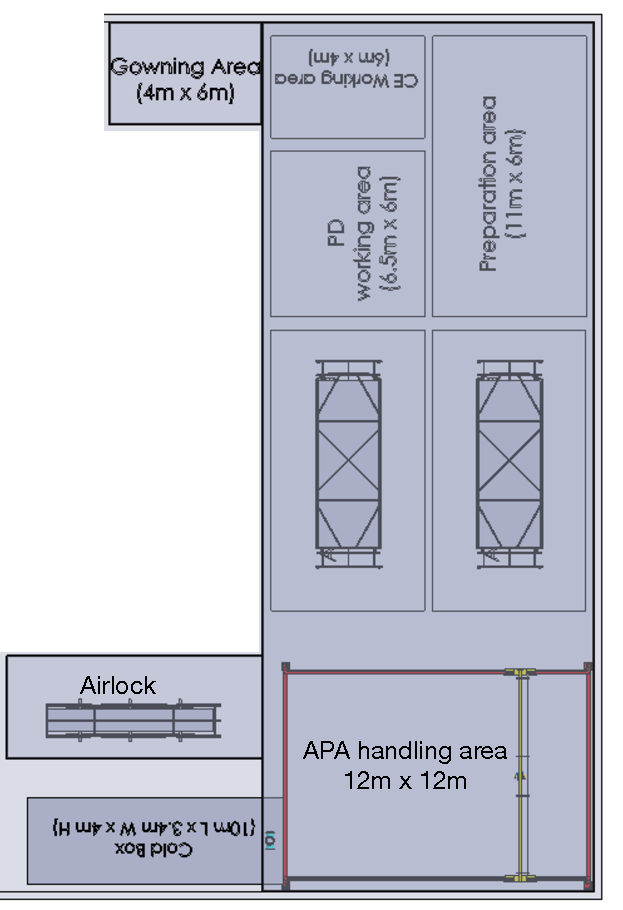
\includegraphics[width=0.8\textwidth]{itf-clean}
\end{dunefigure}

Most the work in the ITF must be done in a cleanroom environment to protect the components from dust and unfiltered light. The cleanliness requirement for the detector components is ISO-8 which corresponds to filtered air with clean lab coats, clean shoes, and hair nets. To protect the photon detector's TPB coating the lights need to be filtered to remove frequencies below 520nm. One possible layout of the cleanroom is shown in Figure \ref{fig:fdsp-tc-itf-clean} . Materials enter the ITF cleanroom through the materials airlock. This area needs to be sufficiently large accommodate the APA transport boxes and allow workers to move around the box to remove the dirty shipping layer and prepare for transport into the cleanroom. Other materials will also through the airlock but they will need much less space. The CE and PD equipment will be moved to the PD work area and preparation area where the components are unpacked and tested. The tests performed are described in detail in the Quality Management section below. The APA will enter cleanroom through the airlock and initially go to the APA handling area where an overhead workstation or gantry crane will be available. The APA will then be removed from the transport box and mounted to a process cart which can rotate the APA horizontally. The process cart will be pushed to one of the two APA integrations areas and then prepared for the installation of the CE and PD. During the integration process the APA will be held horizontal and the PDs will be inserted into the sides while the cold electronic boxes are mounted to the end of the APA. After the component integration the system will be tested and then either moved back to the handling area and boxed for return to the logistics center for storage or inserted into the cold box for further cryogenic testing. 

All the detector  components will arrive at the ITF either from the logistics facility or directly from the factories. Sufficient space will be needed inside the ITF but outside the cleanroom to store several weeks of material and a few boxes of the integrated APA boxes. Additionally a changing room is needed for the workers to change into clean cloths and shoes. The capacity of the changing room should be sufficient for roughly 20 workers in the cleanroom. 

%%%%%%%%%%%%%%%%%%%%%%%%%%%%
\subsection{Quality Management}
\label{sec:fdsp-tc-itf-qaqc}
Extensive testing of the detector components will be performed inside the IFT facility as the APA-PD-CE integration takes place. These tests form a vital part of the quality control process for DUNE. Details of the tests for each of the components are described below.

\subsubsection{Cold Electronics}

\subsubsection{APA}

\subsubsection{Photon Detectors}

%%%%%%%%%%%%%%%%%%%%%%%%%%%%
\subsection{Building Requirements and Infrastructure}
\label{sec:fdsp-tc-itf-req}
The ITF building requirements are summarized in DocDb 11500.
\cite{bib:docdb11500} 

The building to be used as the ITF facility has not been identified at present. In order to assist in identify or designing the ITF building a set of requirements were drafted. The requirements document defines the spaces needed for the integration work while not specifying the final layout of the cleanroom. This will allow the configuration of the cleanroom spaces to be adapted to possible building footprints as candidate buildings are identified. As the building has not been identified yet the cleanroom layout shown in Figure \ref{fig:fdsp-tc-itf-clean} should be taken as a concept and the final layout may change to adapt to the footprint of the final building. The building requirements document\cite{docdb-11500}  defines the minimum spaces for all the operations inside the ITF cleanroom, it defines the space needed for the cold box and the related cryogenic system, it provides guidance for the space needed for material storage outside the cleanroom, and it established the power and other general requirements the building must fulfill. Some requirements depend on the location of the building and the facilities available in the area. For example office space for 20 scientists working in the ITF will be needed in the area but  this would not need to be in the ITF building if local options are available. Some local machining facilities also fall into this category. 

%%%%%%%%%%%%%%%%%%%%%%%%%%%%
\subsection{Safety}
\label{sec:fdsp-tc-itf-safety}


%%%%%%%%%%%%%%%%%%%%%%%%%%%%
\subsection{Cost, Schedule and Risk Analysis}
\label{sec:fdsp-tc-itf-cost}

\fixme{use templates from cost-risk-sched.tex file. Anne}
